\documentclass[12pt, a4paper]{book}
\begin{document}
\chapter{Results}\label{chap:results}
The time has come to test how our networks fare on learning the eight models with DM candidates we are studying: The three mono-$Z'$ models, Dark Higgs (DH), Light Vector (LV) and light Effective Field Theory (EFT) in the Heavy Dark Sector (HDS) and Light Dark Sector (LDS)\footnote{Where HDS and LDS denotes the assumed DM masses as shown in Table \ref{tab:DMass}}, 
the supersymmetric direct slepton production, and the Two Higgs Doublet Model with an additional pseudoscalar $a$ (2HDM + a). As we got better results when using BDTs rather than NNs (see Section \ref{sec:opt_res}), only the BDT will be followed up. \\
\\This chapter showcases the results of both methods we used to train a BDT to classify signal (DM events) and background (SM events). The first method, which we called the model dependent approach, which trains one BDT for each model we have, including all the mass points and simulated samples as seen in Section \ref{chap:DM_sample}. \\
\\The second method, which we called the model independent approach, where we split the dataset in orthogonal Signal Regions (SR). The SRs we studied are
\begin{itemize}
   \item SR1: $m_{ll} >110$ GeV and $E_T^{miss} \in [50, 100]$ GeV
   \item SR2: $m_{ll} >110$ GeV and $E_T^{miss} \in [100, 150]$ GeV
   \item SR3: $m_{ll} >110$ GeV and $E_T^{miss} >150$ GeV
\end{itemize}
To test how well the networks have learned the models we will create a mass exclusion limits for every model. We decided to make a cut of $m_{ll} >110$ GeV for the mono-Z' models when using the model dependent approach to reduce computational time.\\
\\To compare the model independent approach to the model dependent approach we will statistically combine the mass exclusion results for each SR for each final state channel. To navigate through the process we will look at the Dark Higgs Heavy Dark Sector model, using the model dependent method, 
as the model independent method does the same with three SRs. Afterwards we will present the combined exclusion limits for all eight models.


\graphicspath{{../../../Plots/}}
\section{Model dependent approach}\label{sec:Walkthrough}
We conducted a grid search to optimize the BDT and trained the network using 80\% of the SM background samples and 80\% of every different $Z'$ mass sample of the DH HDS model. When training the BDT on the DH HDS model we used the feature importance feature to see which kinematical variables were most important for the BDT in 
categorizing signal (DM events) from background (SM events), this is illustrated in Figure \ref{fig:DH_HDS_feat}. 
\begin{figure}[!ht]
	\centering
      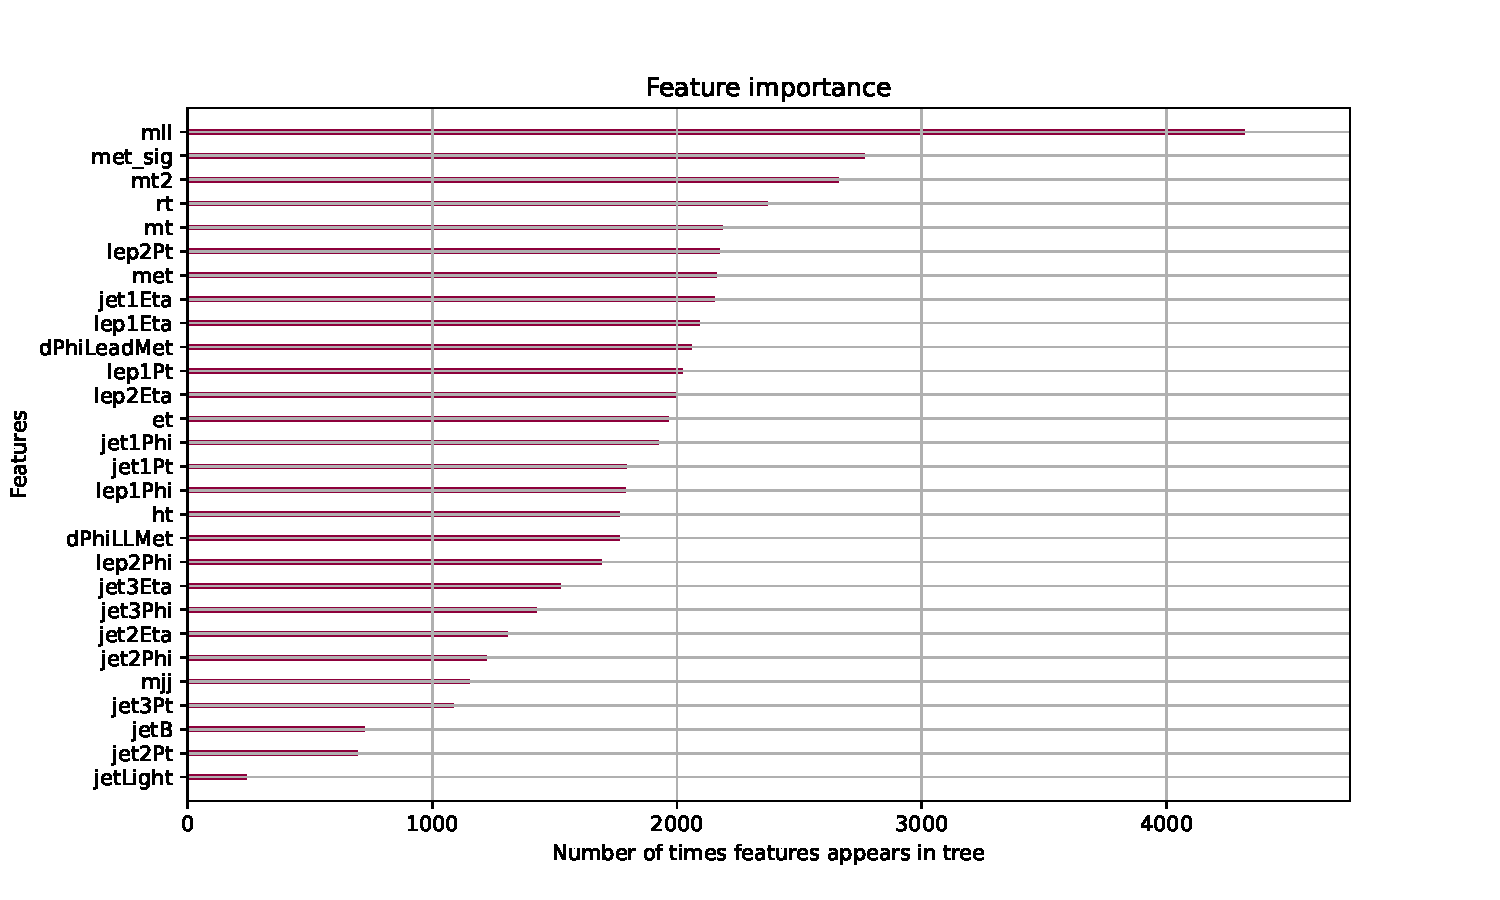
\includegraphics[width=0.8\textwidth]{XGBoost/DH_HDS/feature_importance/weight.pdf}
   \caption[Feature importance for network trained on Z' DH HD model using the model dependent approach]{Feature importance for network trained on Z' DH HD model using the model dependent approach using the weight metric, which shows how many times a feature appears in a tree. The features in this plot use the labeling presented in Table \ref{tab:variables}. 
   To see the feature importance plots with the cover metric, which show the number of samples affected by the split using the feature, and gain metric, which measures the relative contribution of a feature to the network's performance, see Appendix \ref{apx:MDA}.}\label{fig:DH_HDS_feat}
\end{figure}
\\From Figure \ref{fig:DH_HDS_feat} we can see that the most important kinematical variable for the BDT in classifying DM signal from the DH HDS model from SM background was the invariant mass $m_{ll}$, this is what we expect as the DH HDS model is based 
on a mono-$Z'$ theory including a new $Z'$ boson decaying to two leptons, and this includes a resonance on the mass of the $Z'$ as explained by the Breit-Wigner resonance in Eq (\ref{eq:Breit-Wigner}). Furthermore, we see that the three following features are all MET related, which is how we predict to measure the presence of DM. 
These are the MET-significane, $E_T^{miss,sig}$, the stransverse mass $m_{T2}$, and the ratio between MET and hadronic activity $E_T^{miss}/H_T$. Something to note of the features in Figure \ref{fig:DH_HDS_vals} is that we use both $E_T^{miss}$ and $E_T^{miss,sig}$ which are correlated, the reason for using both is because the BDT 
might find that one is better at classifying DM signal from SM background when training on other models.\\
\\To showcase how the network categorizes signal from background the validation plots in Figure \ref{fig:DH_HDS_vals} is made on the 20\% test samples for some the signal samples, together with the SM predictions and data. The data in the plots will not be shown for an output score of 0.6 or greater as this is the signal region, and 
we need to go through an unblinding procedure to show data in this region.\\
\begin{figure}[!ht]
	\centering
	\begin{subfigure}[b]{0.49\textwidth}
      \centering
      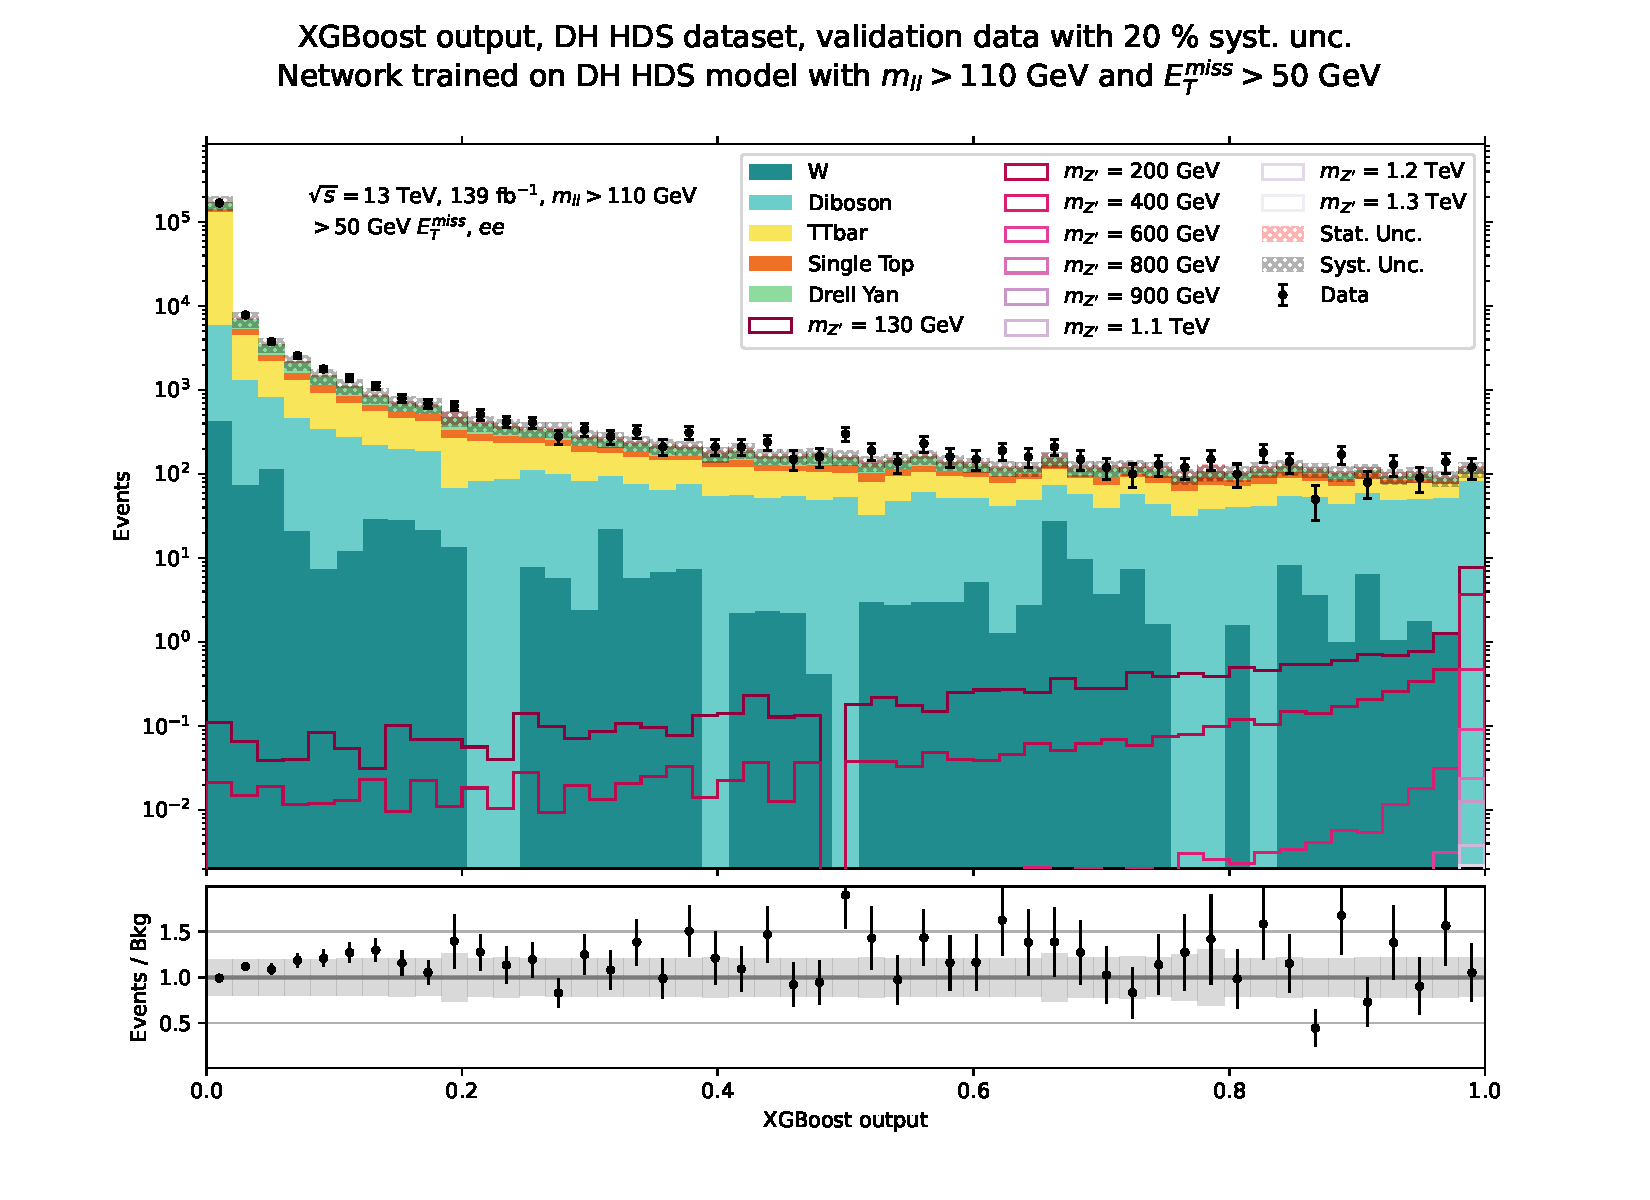
\includegraphics[width=1\textwidth]{XGBoost/DH_HDS/VAL_ee.pdf}
      \end{subfigure}
   \hfill
   \begin{subfigure}[b]{0.49\textwidth}
      \centering
      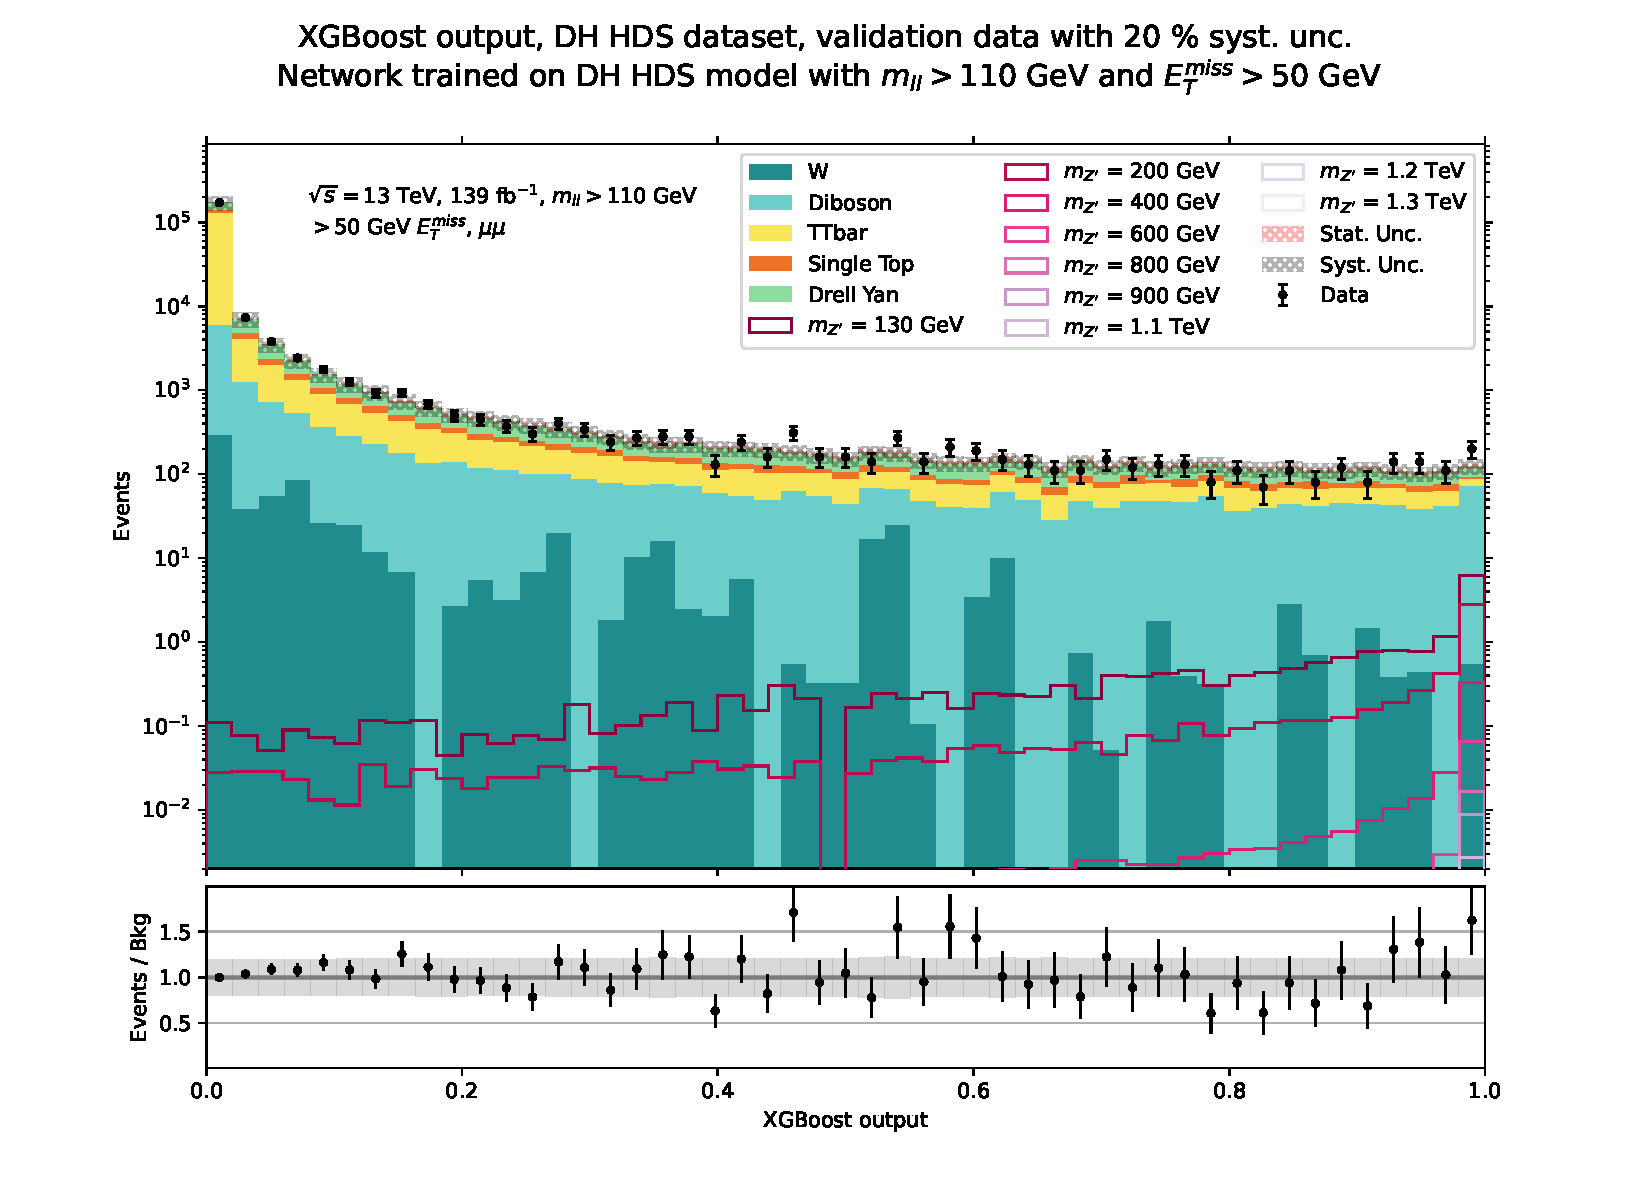
\includegraphics[width=1\textwidth]{XGBoost/DH_HDS/VAL_uu.pdf}
      \end{subfigure}
   \caption[Validation plots for network trained on Z' DH HDS model using the model dependent approach. ]{Validation plots for network trained on Z' DH HDS model using the model dependent approach. The validation plots show the distribution of the BDT score for every event from 0-1, where 1 is signal. On the left we have the results for the $ee$ channel, and on the right we have the result for the $\mu\mu$ channel. Both results were 
   trained by the same network consisting of a general dilepton final state.}\label{fig:DH_HDS_vals}
\end{figure}
\\While the validation plot might indicate that the network is not doing an impressive job at sorting signal from background, we can actually see how well the network learns the different mass points on the DH HDS model by looking at the ROC curves for each mass point, shown in Figure \ref{fig:DH_HDS_ROCS} for the $ee$ channel (left) and the $\mu\mu$ channel (right). 
Here we see that the network struggles a tiny bit to learn the DH HDS models with the lowest $m_{Z'}$, but the AUC score is still 0.96, meaning that it actually learned to sort the signal from SM background.\\
\begin{figure}[!ht]
	\centering
	\begin{subfigure}[b]{0.49\textwidth}
      \centering
      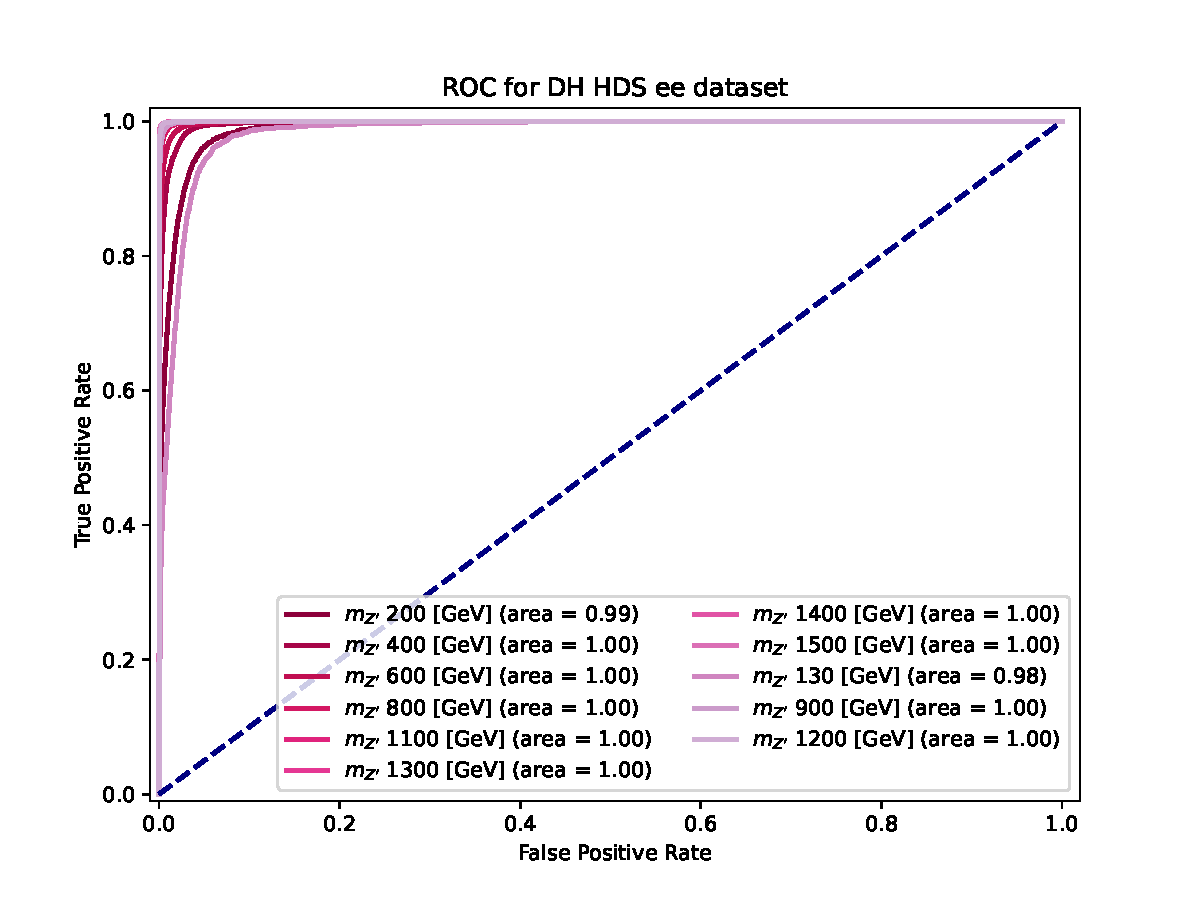
\includegraphics[width=1\textwidth]{XGBoost/DH_HDS/ROC_ee.pdf}
      \end{subfigure}
   \hfill
   \begin{subfigure}[b]{0.49\textwidth}
      \centering
      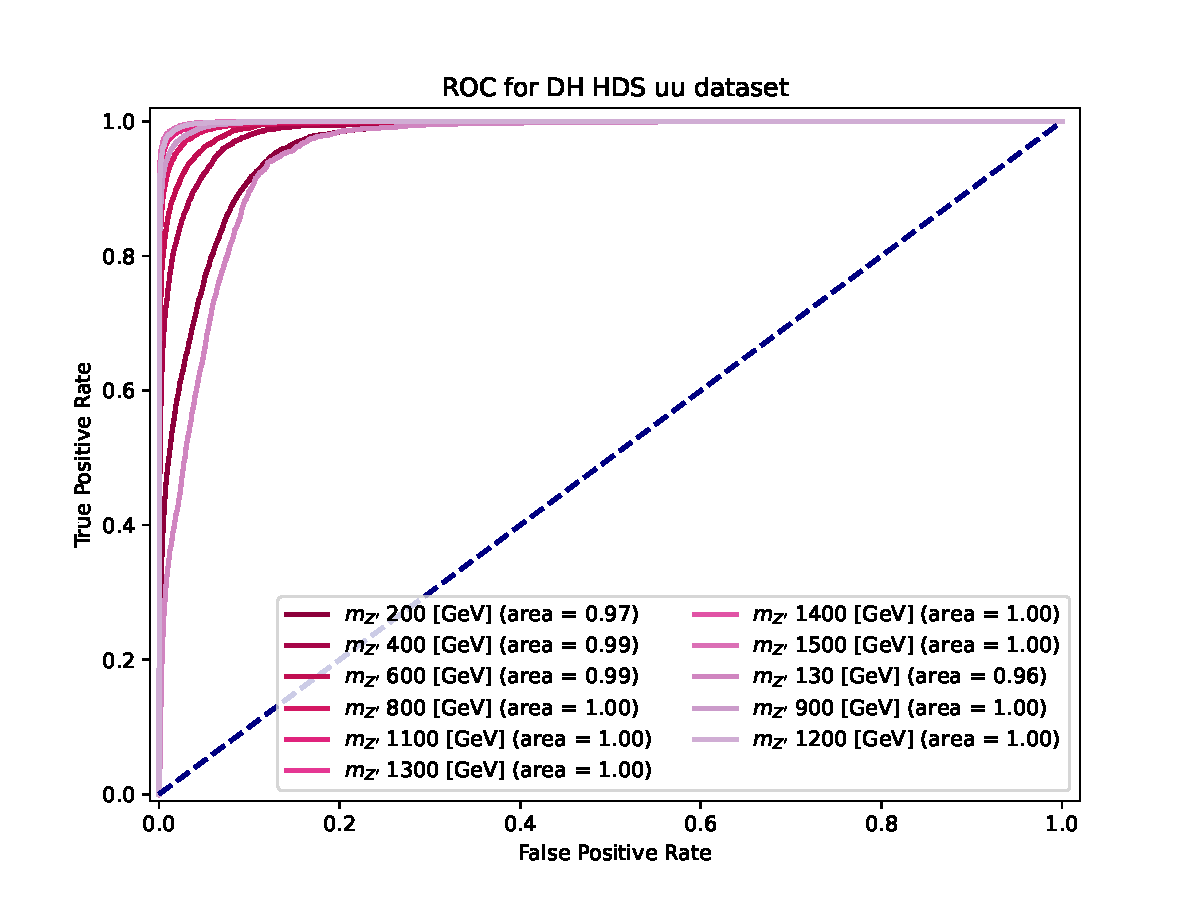
\includegraphics[width=1\textwidth]{XGBoost/DH_HDS/ROC_uu.pdf}
      \end{subfigure}
   \caption[ROC plots for every Z' mass point on network trained on Z' DH HDS model using the model dependent approach]{ROC plots for every Z' mass point on network trained on Z' DH HDS model using the model dependent approach. On the left we have the results for the $ee$ channel, and on the right we have the result for the $\mu\mu$ channel. Both results were 
   trained by the same network consisting of a general dilepton final state. The dashed blue line showcases the score of a random guess (AUC = 0.5)}\label{fig:DH_HDS_ROCS}
\end{figure}
\\To define the region we will use to set any expected exclusion limits, we can choose the validation plot bin that gives us the highest expected significance. In Figure \ref{fig:DH_HDS_exp_sig} we show the calculation of the expected significance as a function of the lower cut on the BDT output 
for a few mass points.
\begin{figure}[!ht]
	\centering
	\begin{subfigure}[b]{0.49\textwidth}
      \centering
      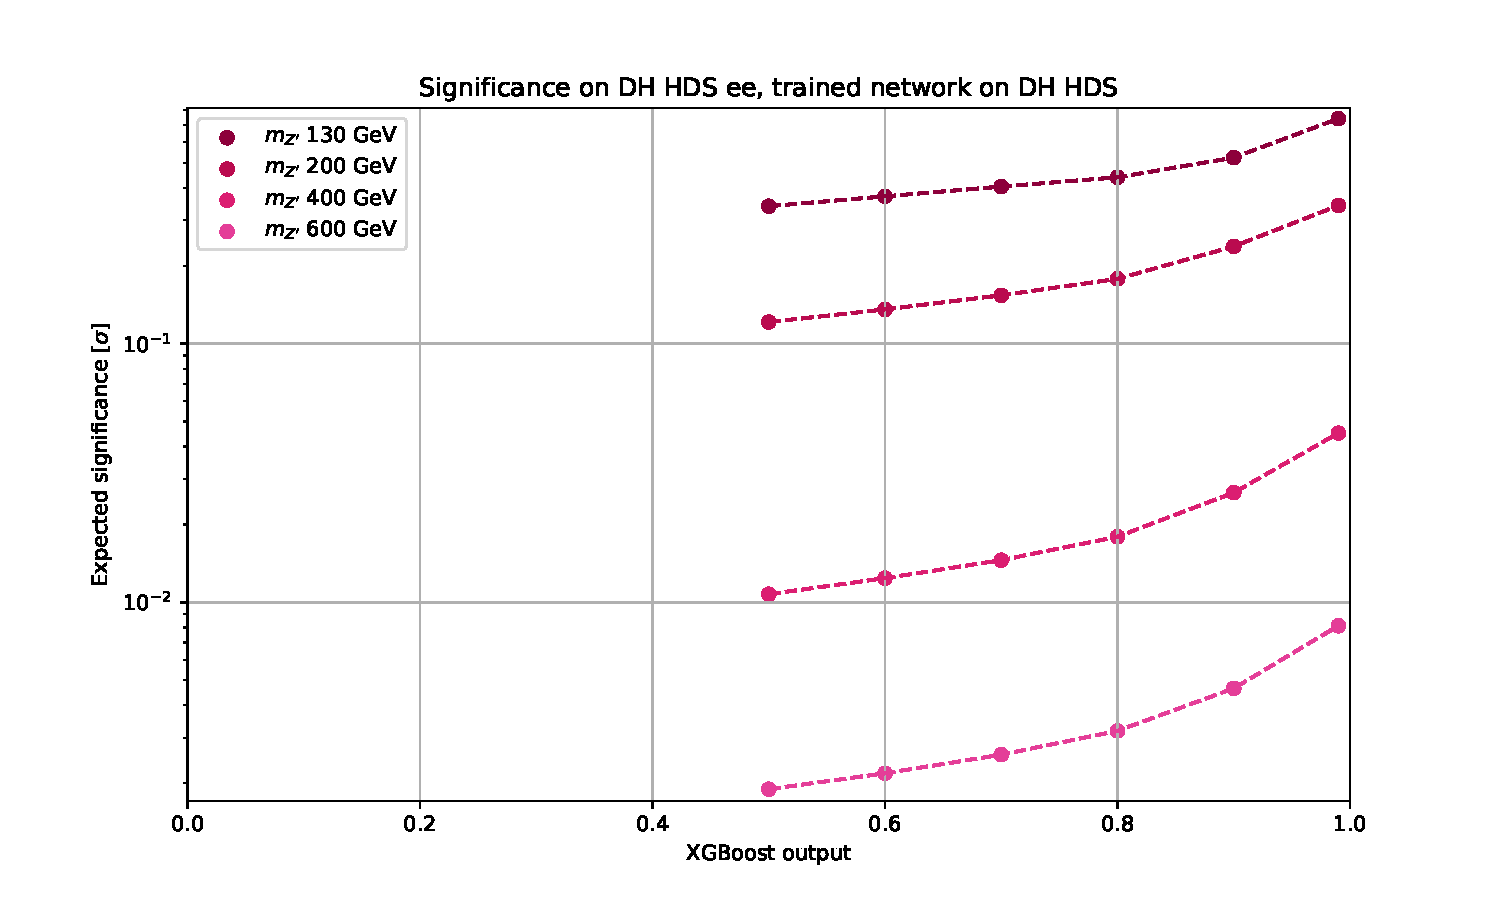
\includegraphics[width=1\textwidth]{XGBoost/DH_HDS/EXP_SIG_ee.pdf}
      \end{subfigure}
   \hfill
   \begin{subfigure}[b]{0.49\textwidth}
      \centering
      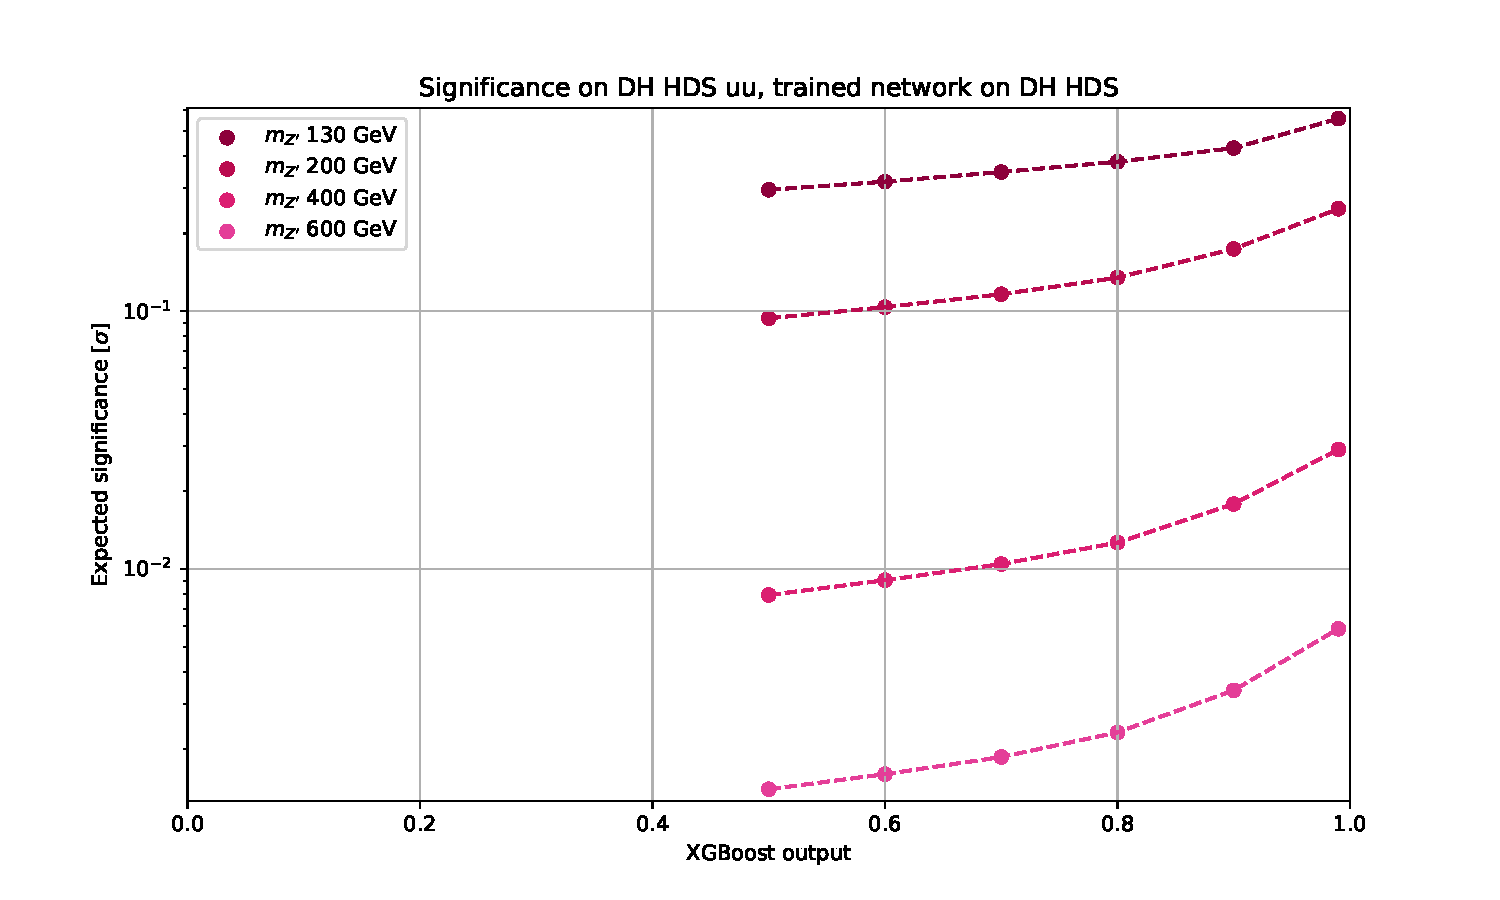
\includegraphics[width=1\textwidth]{XGBoost/DH_HDS/EXP_SIG_uu.pdf}
      \end{subfigure}
   \caption{Expected significance plots for Z' mass points as a function on the lower cut on the BDT output on BDT trained on the Z' DH HDS model using the model dependent approach}\label{fig:DH_HDS_exp_sig}
\end{figure}
\\In Figure \ref{fig:DH_HDS_exp_sig} we see that we get the best expected significance of approximately 0.7$\sigma$ (without uncertainties), even though the network got an AUC score of 0.96 for the mass point on the muon channel. From this we see that even with an AUC of 0.96 we do not manage to exclude the model.\\
\\As the last bin of the BDT output on the validation plots scores the greatest expected significance for every $m_{Z'}$, we can effectively make a cut based on the BDT score. Counting the number of events in this last bin, as well as their uncertainties we can calculate a mass exclusion for both the $ee$ and $\mu\mu$ channels. 
Utilizing Bayesian statistics with the signal+background hypothesis, we can use the values of $\varepsilon_{\text{sig}}$, $N_{\text{bkg}}$ and $\sigma B$ from Table \ref{tab:stat_vals_DH_HDS} for each mass points for each leptonic channel, to make a 95\% CL expected exclusion. \\
\begin{table}[!ht]\centering\caption[Inputs for the $Z'h_D\rightarrow l^+l^-\chi\chi$ HDS $\sigma B$ calculations]{Inputs for the $Z'h_D\rightarrow l^+l^-\chi\chi$ HDS $\sigma B$ calculations. The first three columns are the $Z'$ mass, the theoretical cross-section times branching ratio $\sigma B$, and what $Z'$ decay channel we are looking at. 
   The next two are $\varepsilon_{\text{sig}}$, which is the signal selection efficiency, and $N_{\text{sig}}$, which is the predicted number of signal events after the cuts. The last column is the number of background events, $N_{\text{bkg}}$. 
   The uncertainties of $\varepsilon_{\text{sig}}$, $N_{\text{sig}}$ and $N_{\text{bkg}}$ are statistical with an assumed 20\% flat systematic uncertainty. The MET threshold is $E_{\text{T,min}}^{\text{miss}}=50$GeV and the invariant mass threshold is $m_{ll}^{min}=110$GeV 
   and is the same for all inputs.}
   \small\begin{tabular}{@{}ccc|ccc@{}}
      \midrule\midrule 
         $m_{Z'}$ [GeV] & $\sigma B$ [fb] & Channel & $\varepsilon_{\text{sig}}$ $[\times10^{-1}]$& $N_{\text{sig}}$ & $N_{\text{bkg}}$ \\\midrule\midrule
         \multirow{2}{*}[-2\baselineskip]{130}& \multirow{2}{*}[-2\baselineskip]{$1.11$}& $ee$ & $0.25\pm0.05$ & $7.80\pm1.58$ & $108.4\pm23.0$ \\ 
         & & $\mu\mu$ & $0.20\pm0.04$ & $6.28\pm1.27$ & $124.9\pm26.1$ \\ \midrule
         \multirow{2}{*}[-2\baselineskip]{200}& \multirow{2}{*}[-2\baselineskip]{$2.46\times10^{-1}$}& $ee$ & $0.54\pm0.11$ & $3.67\pm0.74$ & $114.1\pm24.4$ \\ 
         & & $\mu\mu$ & $0.41\pm0.08$ & $2.78\pm0.56$ & $123.2\pm25.8$ \\ \midrule
         \multirow{2}{*}[-2\baselineskip]{400}& \multirow{2}{*}[-2\baselineskip]{$1.49\times10^{-2}$}& $ee$ & $1.13\pm0.23$ & $4.67\times10^{-1}\pm9.37\times10^{-2}$ & $107.0\pm23.4$ \\ 
         & & $\mu\mu$ & $0.79\pm0.16$ & $3.29\times10^{-1}\pm6.60\times10^{-2}$ & $127.5\pm26.6$ \\ \midrule
         \multirow{2}{*}[-2\baselineskip]{600}& \multirow{2}{*}[-2\baselineskip]{$2.35\times10^{-3}$}& $ee$ & $1.40\pm0.28$ & $9.12\times10^{-2}\pm1.83\times10^{-2}$ & $126.3\pm26.7$ \\ 
         & & $\mu\mu$ & $1.01\pm0.20$ & $6.59\times10^{-2}\pm1.32\times10^{-2}$ & $126.3\pm26.3$ \\ \midrule
         \multirow{2}{*}[-2\baselineskip]{800}& \multirow{2}{*}[-2\baselineskip]{$5.43\times10^{-4}$}& $ee$ & $1.59\pm0.32$ & $2.40\times10^{-2}\pm4.81\times10^{-3}$ & $118.8\pm25.6$ \\ 
         & & $\mu\mu$ & $1.11\pm0.22$ & $1.67\times10^{-2}\pm3.36\times10^{-3}$ & $113.2\pm23.6$ \\ \midrule
         \multirow{2}{*}[-2\baselineskip]{900}& \multirow{2}{*}[-2\baselineskip]{$2.82\times10^{-4}$}& $ee$ & $1.60\pm0.32$ & $1.25\times10^{-2}\pm2.51\times10^{-3}$ & $119.3\pm25.7$ \\ 
         & & $\mu\mu$ & $1.12\pm0.22$ & $8.78\times10^{-3}\pm1.76\times10^{-3}$ & $114.8\pm24.0$ \\ \midrule
         \multirow{2}{*}[-2\baselineskip]{1100}& \multirow{2}{*}[-2\baselineskip]{$8.40\times10^{-5}$}& $ee$ & $1.63\pm0.33$ & $3.81\times10^{-3}\pm7.64\times10^{-4}$ & $114.3\pm24.4$ \\ 
         & & $\mu\mu$ & $1.16\pm0.23$ & $2.70\times10^{-3}\pm5.42\times10^{-4}$ & $118.6\pm24.7$ \\ \midrule
         \multirow{2}{*}[-2\baselineskip]{1200}& \multirow{2}{*}[-2\baselineskip]{$4.75\times10^{-5}$}& $ee$ & $1.65\pm0.33$ & $2.18\times10^{-3}\pm4.37\times10^{-4}$ & $118.4\pm25.1$ \\ 
         & & $\mu\mu$ & $1.14\pm0.23$ & $1.50\times10^{-3}\pm3.01\times10^{-4}$ & $125.6\pm26.3$ \\ \midrule
         \multirow{2}{*}[-2\baselineskip]{1300}& \multirow{2}{*}[-2\baselineskip]{$2.73\times10^{-5}$}& $ee$ & $1.69\pm0.34$ & $1.28\times10^{-3}\pm2.57\times10^{-4}$ & $123.9\pm26.5$ \\ 
         & & $\mu\mu$ & $1.15\pm0.23$ & $8.72\times10^{-4}\pm1.75\times10^{-4}$ & $130.7\pm27.2$ \\ \midrule
         \multirow{2}{*}[-2\baselineskip]{1400}& \multirow{2}{*}[-2\baselineskip]{$1.60\times10^{-5}$}& $ee$ & $1.67\pm0.33$ & $7.43\times10^{-4}\pm1.49\times10^{-4}$ & $115.8\pm24.5$ \\ 
         & & $\mu\mu$ & $1.16\pm0.23$ & $5.15\times10^{-4}\pm1.03\times10^{-4}$ & $125.4\pm26.1$ \\ \midrule
         \multirow{2}{*}[-2\baselineskip]{1500}& \multirow{2}{*}[-2\baselineskip]{$9.42\times10^{-6}$}& $ee$ & $1.69\pm0.34$ & $4.44\times10^{-4}\pm8.90\times10^{-5}$ & $123.9\pm26.5$ \\ 
         & & $\mu\mu$ & $1.13\pm0.23$ & $2.97\times10^{-4}\pm5.96\times10^{-5}$ & $130.7\pm27.2$ \\
      \midrule\midrule
   \end{tabular}
   \label{tab:stat_vals_DH_HDS}
\end{table}
\\The mass exclusion limits can be seen in Figure \ref{fig:DH_HDS_exclusion_ee_uu} for the $ee$ (left) and $\mu\mu$ (right) channel for Z' Dark Higgs Heavy Dark Sector model using the model dependent approach. The y-axis of both plots represents the cross-section times branching ratio of the process we are studying. 
The x-axis is the mass of the $Z'$ boson. We did not interpolate between the available masses we had simulated, and have rather just connected the values calculated for each mass point in Table \ref{tab:stat_vals_DH_HDS} by connecting the points. There we see the expected 95\% CL limit using 
the values of from Table \ref{tab:stat_vals_DH_HDS} with a 1$\sigma$ and 2$\sigma$ deviation. Included in the plots we show how the exclusions look when varying the value of the lepton coupling $g_l$ between the leptons and the $Z'$ boson. The simulated events in this thesis utilized the value $g_l=$ 0.01, 
we increase this coupling to 0.05 and 0.1 to see how the exclusions change.\\
\\We see that we cannot exclude any mass point of the DH HDS model (as the dashed red lines do not cross the dashed black line) when the lepton coupling is set to $g_l=$ 0.01, we can however see that as we increase the lepton coupling, 
we can exclude more points. The highest mass exclusion in both the $ee$ and $\mu\mu$ channel is roughly at $m_{Z'}=300$ GeV (meaning we exclude masses where the dashed line is above the expected limit) when setting $g_{l}=0.1$
\clearpage
\begin{figure}[!ht]
	\centering
   \begin{subfigure}[b]{0.49\textwidth}
      \centering
      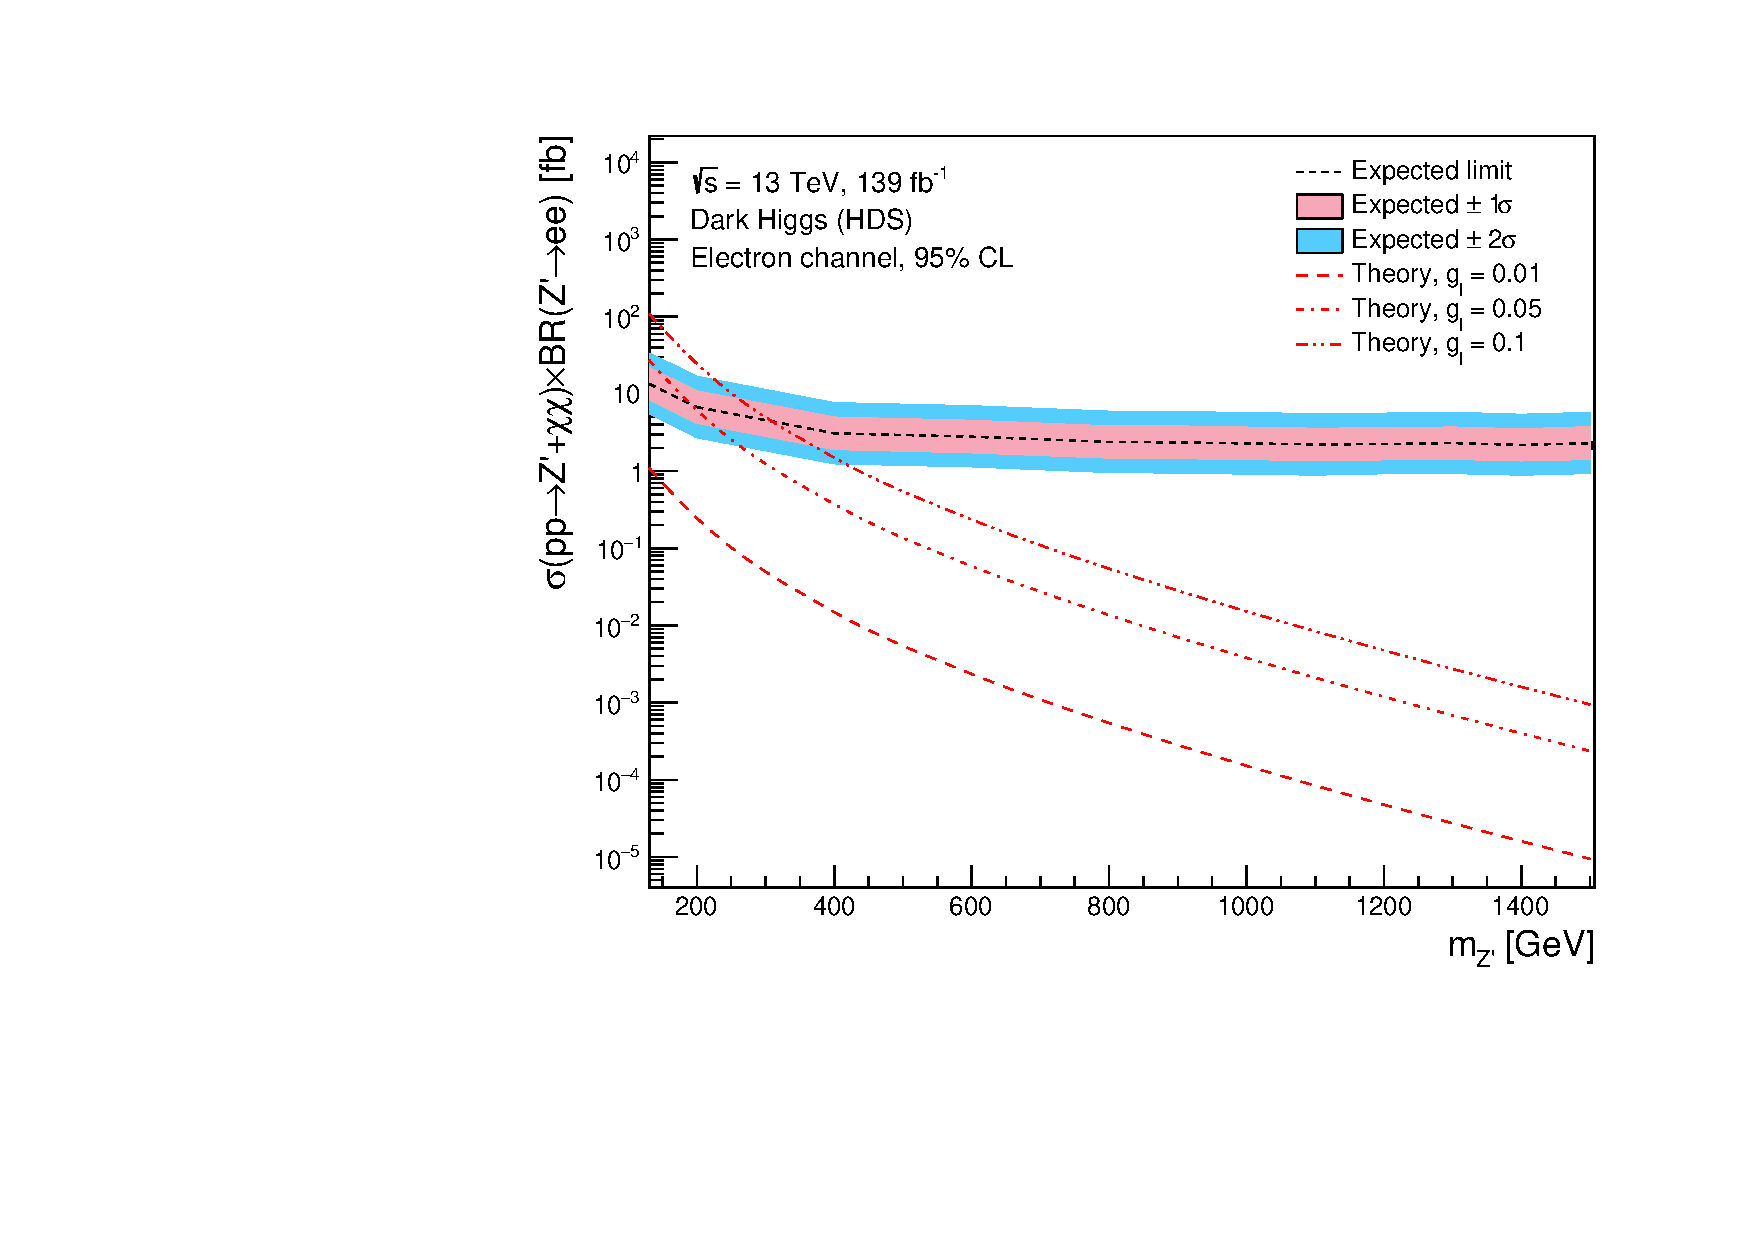
\includegraphics[width=1\textwidth]{Limits/DH_HDS/mass_exclusion_ee.pdf}
      \end{subfigure}
   \hfill
   \begin{subfigure}[b]{0.49\textwidth}
      \centering
      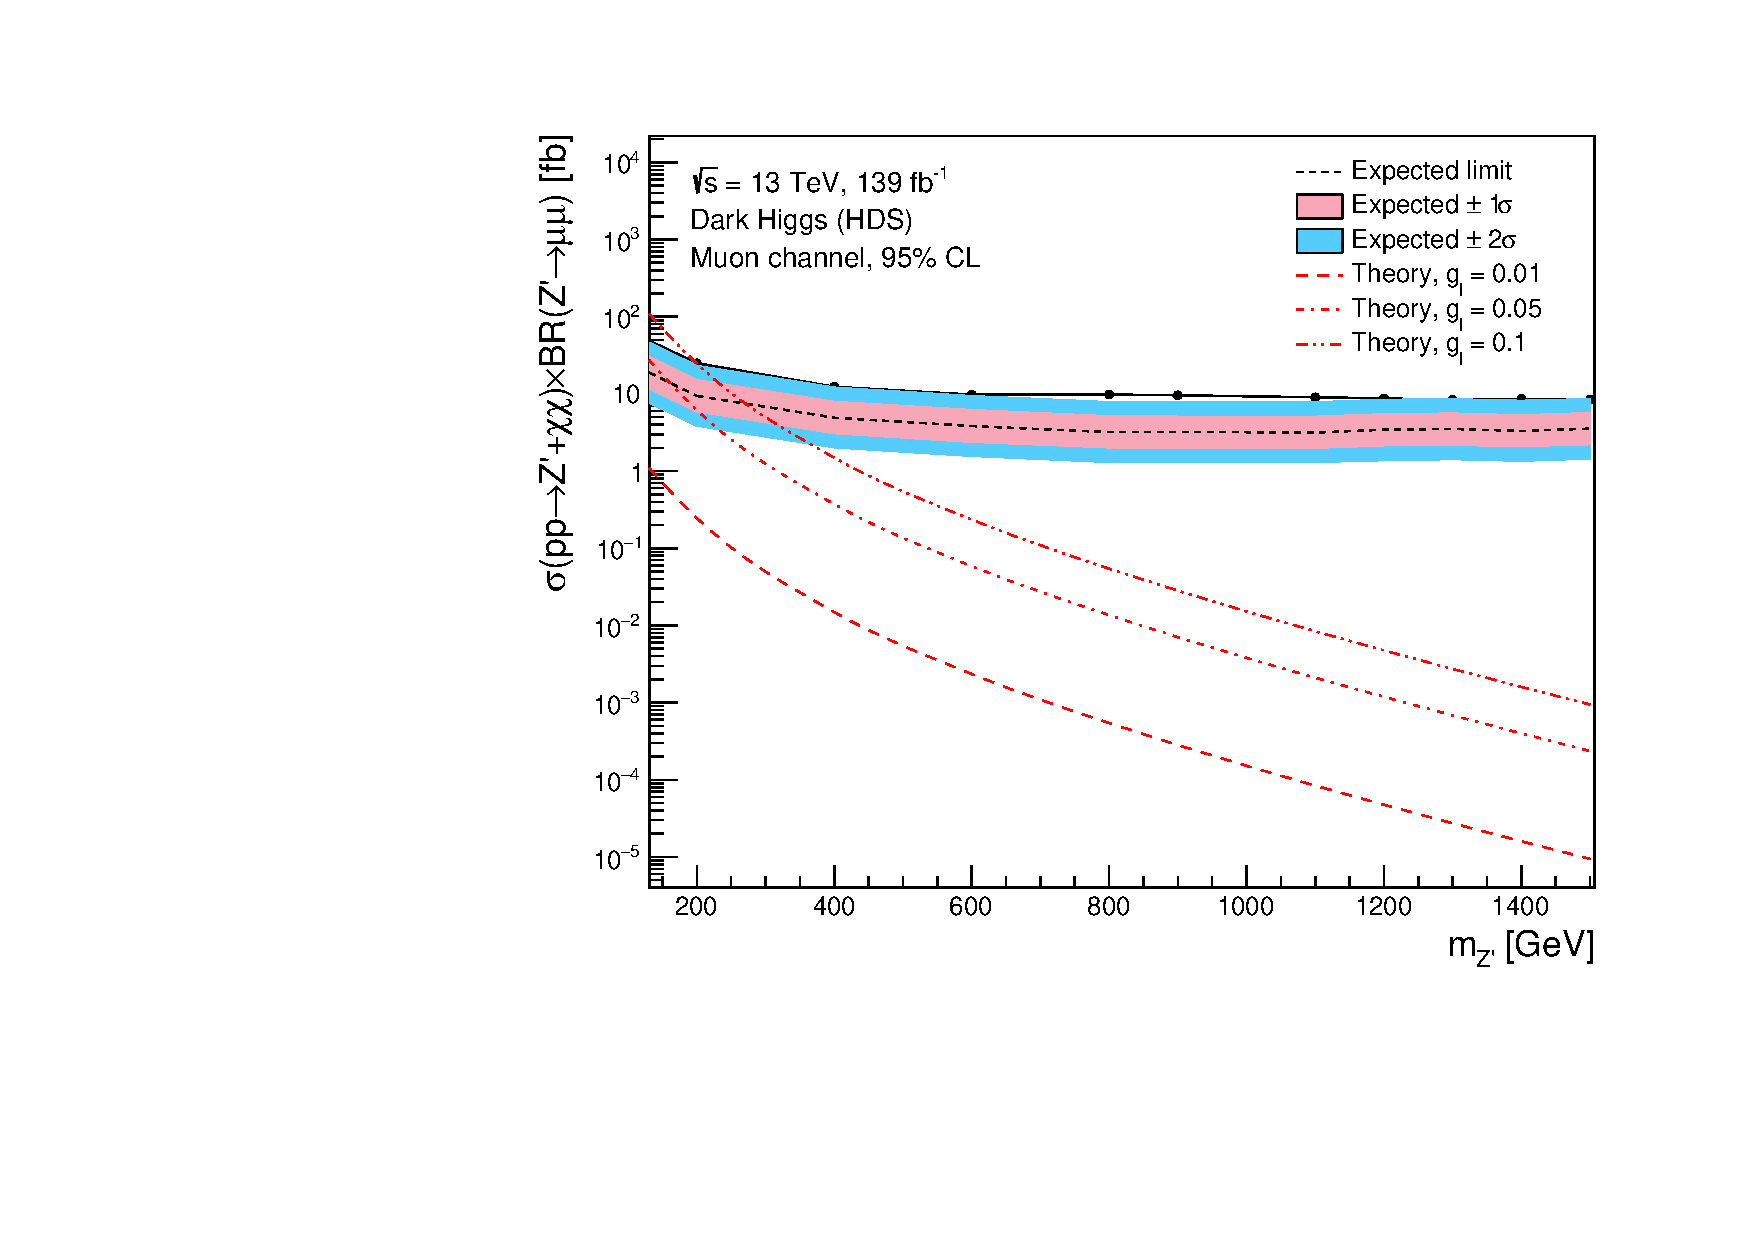
\includegraphics[width=1\textwidth]{Limits/DH_HDS/mass_exclusion_uu.pdf}
      \end{subfigure}
   \caption[Mass exclusion limits of $ee$ and $\mu\mu$ channel for Z' DH HDS model using the model dependent approach]{Mass exclusion limits of $ee$ (left) and $\mu\mu$ (right) channel for Z' Dark Higgs Heavy Dark Sector model using the model dependent approach. The y-axis of both plots represents the cross-section times branching ratio of the process we are studying. The x-axis is the mass of the $Z'$ boson. We did not interpolate between the available masses we had simulated, 
   and have rather just connected the values calculated for each mass point in Table \ref{tab:stat_vals_DH_HDS} by connecting the points. The dashed black line is the expected 95\% CL limit calculated using the values of from Table \ref{tab:stat_vals_DH_HDS} with a 1$\sigma$ and 2$\sigma$ deviation. 
   The different dashed lines represent the theoretical cross-section times branching ratio of the process when varying the value of the lepton coupling $g_l$ between the leptons and the $Z'$ boson. The simulated events in this thesis utilized the value $g_l=$ 0.01, we include the cross-section times branching ratio when increasing this coupling to 0.05 and 0.1 to see how the exclusions change.  }\label{fig:DH_HDS_exclusion_ee_uu}
\end{figure}
\noindent When changing the lepton coupling $g_l$ we have assumed that the efficiency of the cuts stays the same, as well as the number of background events in the last bin. This assumption is noteworthy due to the fact that if we increased the lepton coupling value of our model, this would increase the branching ratio 
of the leptonic decays. Meaning that when using MC to simulate we would have gotten more events. As one of the greatest challenges in this thesis was the imbalanced dataset, this fact would have helped mitigate the problem. 
In addition, a general rule of thumb in ML is that the more statistics one has when training a network, the better the network will learn. 
This means that if we instead simulated new events with a greater lepton coupling, the network could have achieved a greater efficiency. However, due to time constrains on this thesis we did not have the chance to explore the possibility of simulating more events, with varying lepton couplings.
\clearpage\noindent We can furthermore statistically combine both of the $ee$ and $\mu\mu$ results from Figure \ref{fig:DH_HDS_exclusion_ee_uu} to get the exclusion on a dilepton final state. Following this method for all other seven models\footnote{For more plots look at the GitHub repo: in \href{https://github.com/rubenguevara/Master-Thesis/tree/master/Plots/XGBoost/DH_HDS}{https://github.com/rubenguevara/Master-Thesis\\/tree/master/Plots/XGBoost/DH\_HDS} changing "DH\_HDS" for the model of interest} 
we can get the results in Figure \ref{fig:model_dep_excl} for the direct slepton production and 2HDM + a (only showing $\tan\beta$ = 30) and in Figure \ref{fig:model_dep_mono_Zp_excl} for the mono-$Z'$ models.
\begin{figure}[!ht]
	\centering
	\begin{subfigure}[b]{0.49\textwidth}
      \centering
      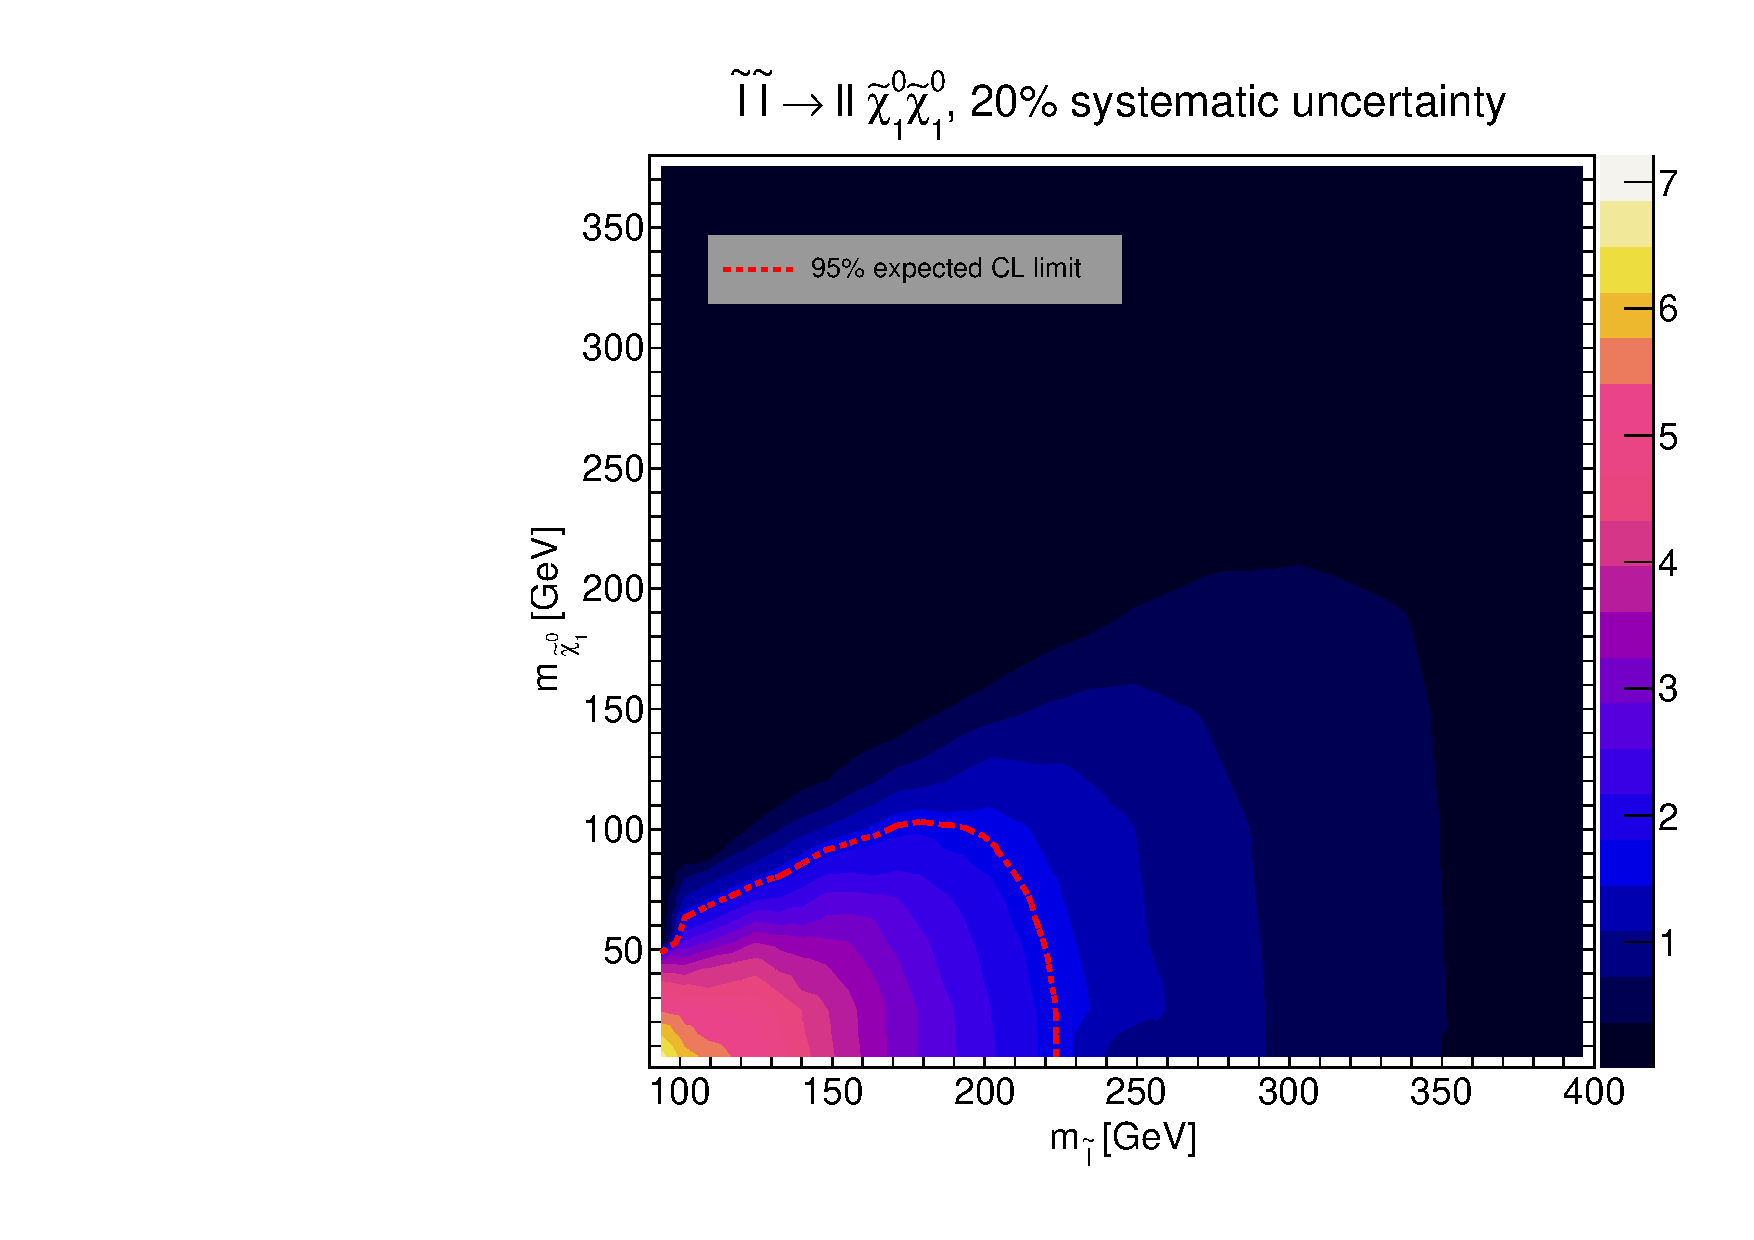
\includegraphics[width=1\textwidth]{Limits/SlepSlep/SlepSlep_ll.pdf}
   \end{subfigure}
   \hfill
   \begin{subfigure}[b]{0.49\textwidth}
      \centering
      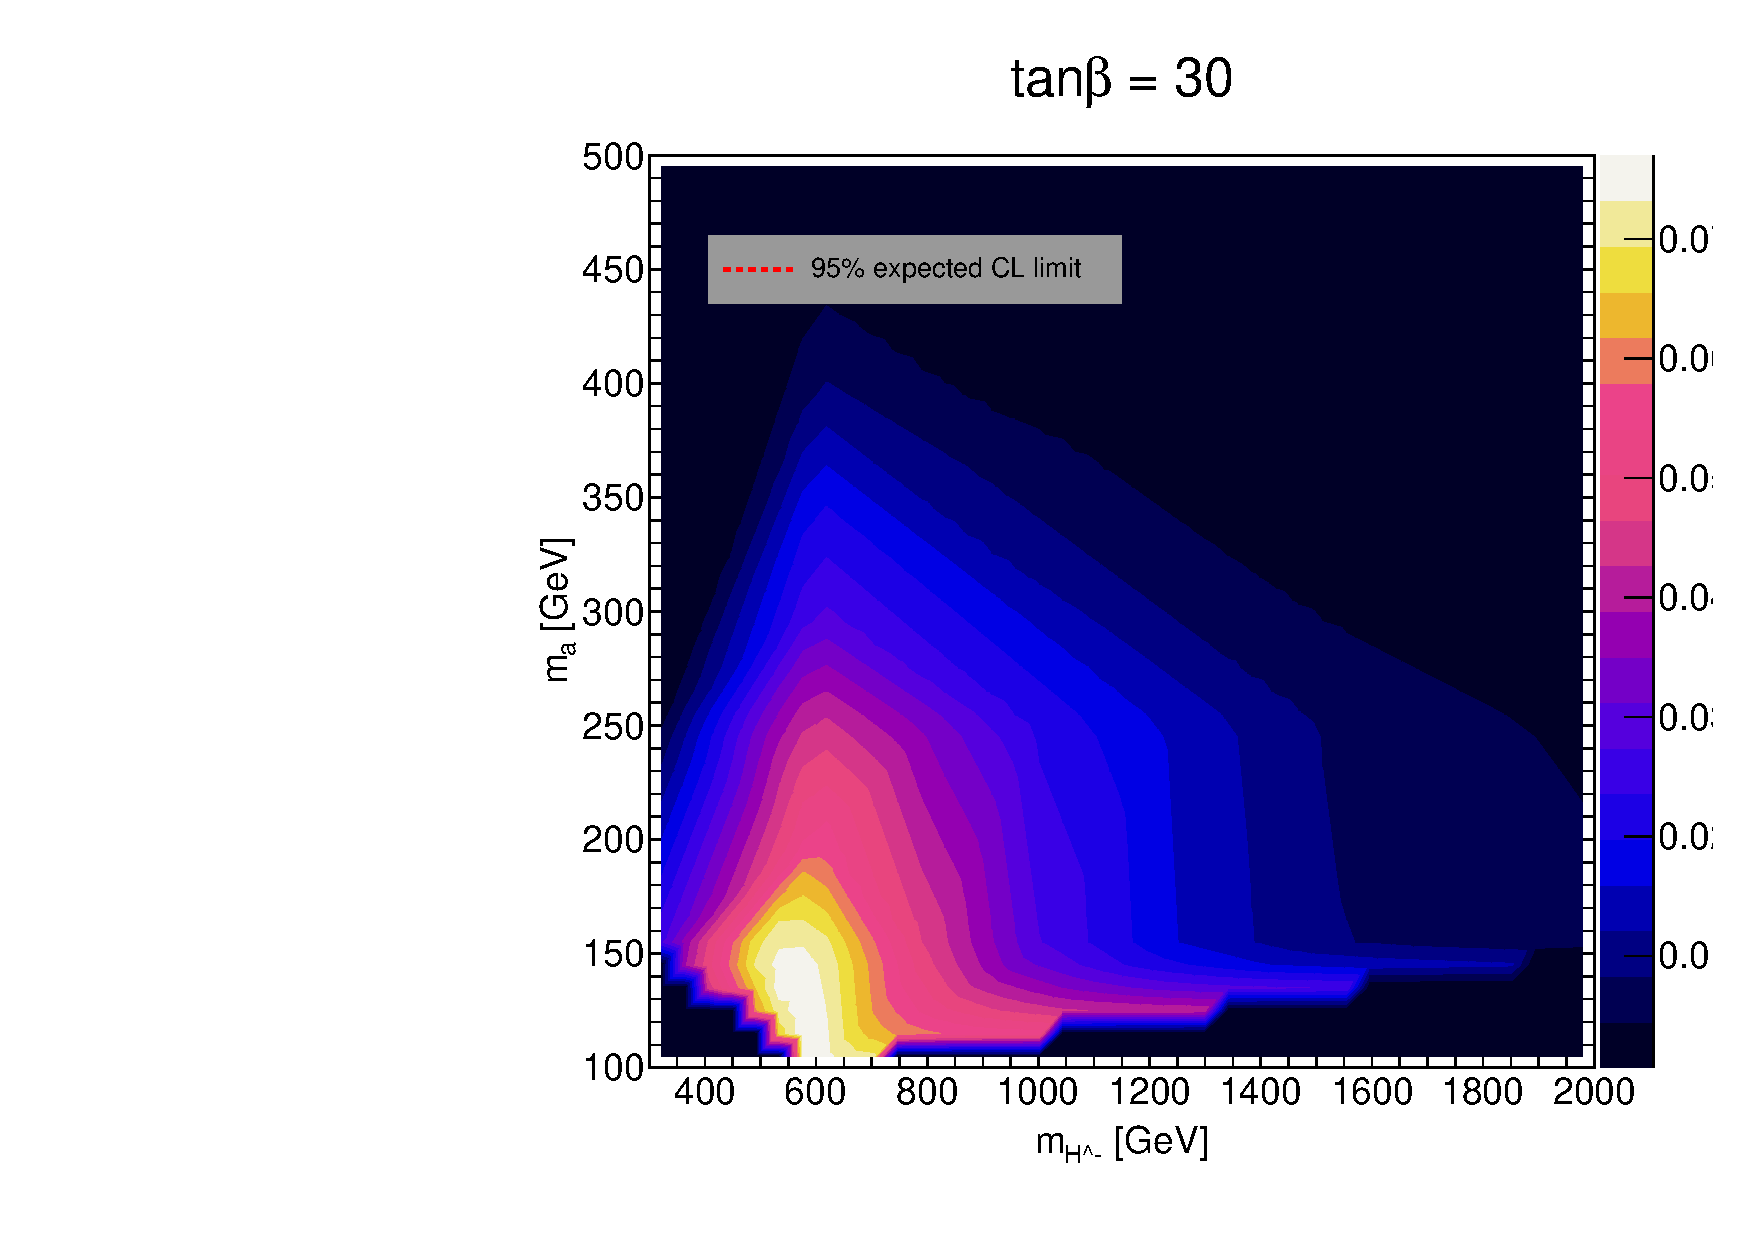
\includegraphics[width=1\textwidth]{Limits/2HDM/2HDM_ll_tb30.pdf}
   \end{subfigure}
   \caption[Mass exclusion limits of combined $ee$ and $\mu\mu$ channel for direct slepton production and 2HDM + a using the model dependent approach]{
      Mass exclusion limits of combined $ee$ and $\mu\mu$ channel for direct slepton production (left) and 2HDM + a for $\tan\beta=30$ (right) using the model dependent approach. The plots here have the two varying masses as the axes, the z-axis is the expected significance calculated using Eq. (\ref{eq:significance}) with uncertainties. The expected 95\% CL limit was chosen using Frequentist statistics using the significance $Z=$ 1.645.   
      For the direct slepton production model we have the slepton mass, $m_{\tilde{\ell}}$, on the x-axis, and the neutralino mass on $m_{\tilde{\chi}_1^0}$ the y-axis. 
      For the 2HDM + a model we have the charged Higgs mass, $m_{H^-}$, on the x-axis, and the pseudoscalar $a$ mass $m_{a}$ on the y-axis. To see the exclusions for the other values of $\tan\beta$ on the 2HDM + a model see Appendix \ref{apx:MDA}.  
      }\label{fig:model_dep_excl}
\end{figure}
\begin{figure}[!ht]
	\centering
	\begin{subfigure}[b]{0.49\textwidth}
      \centering
      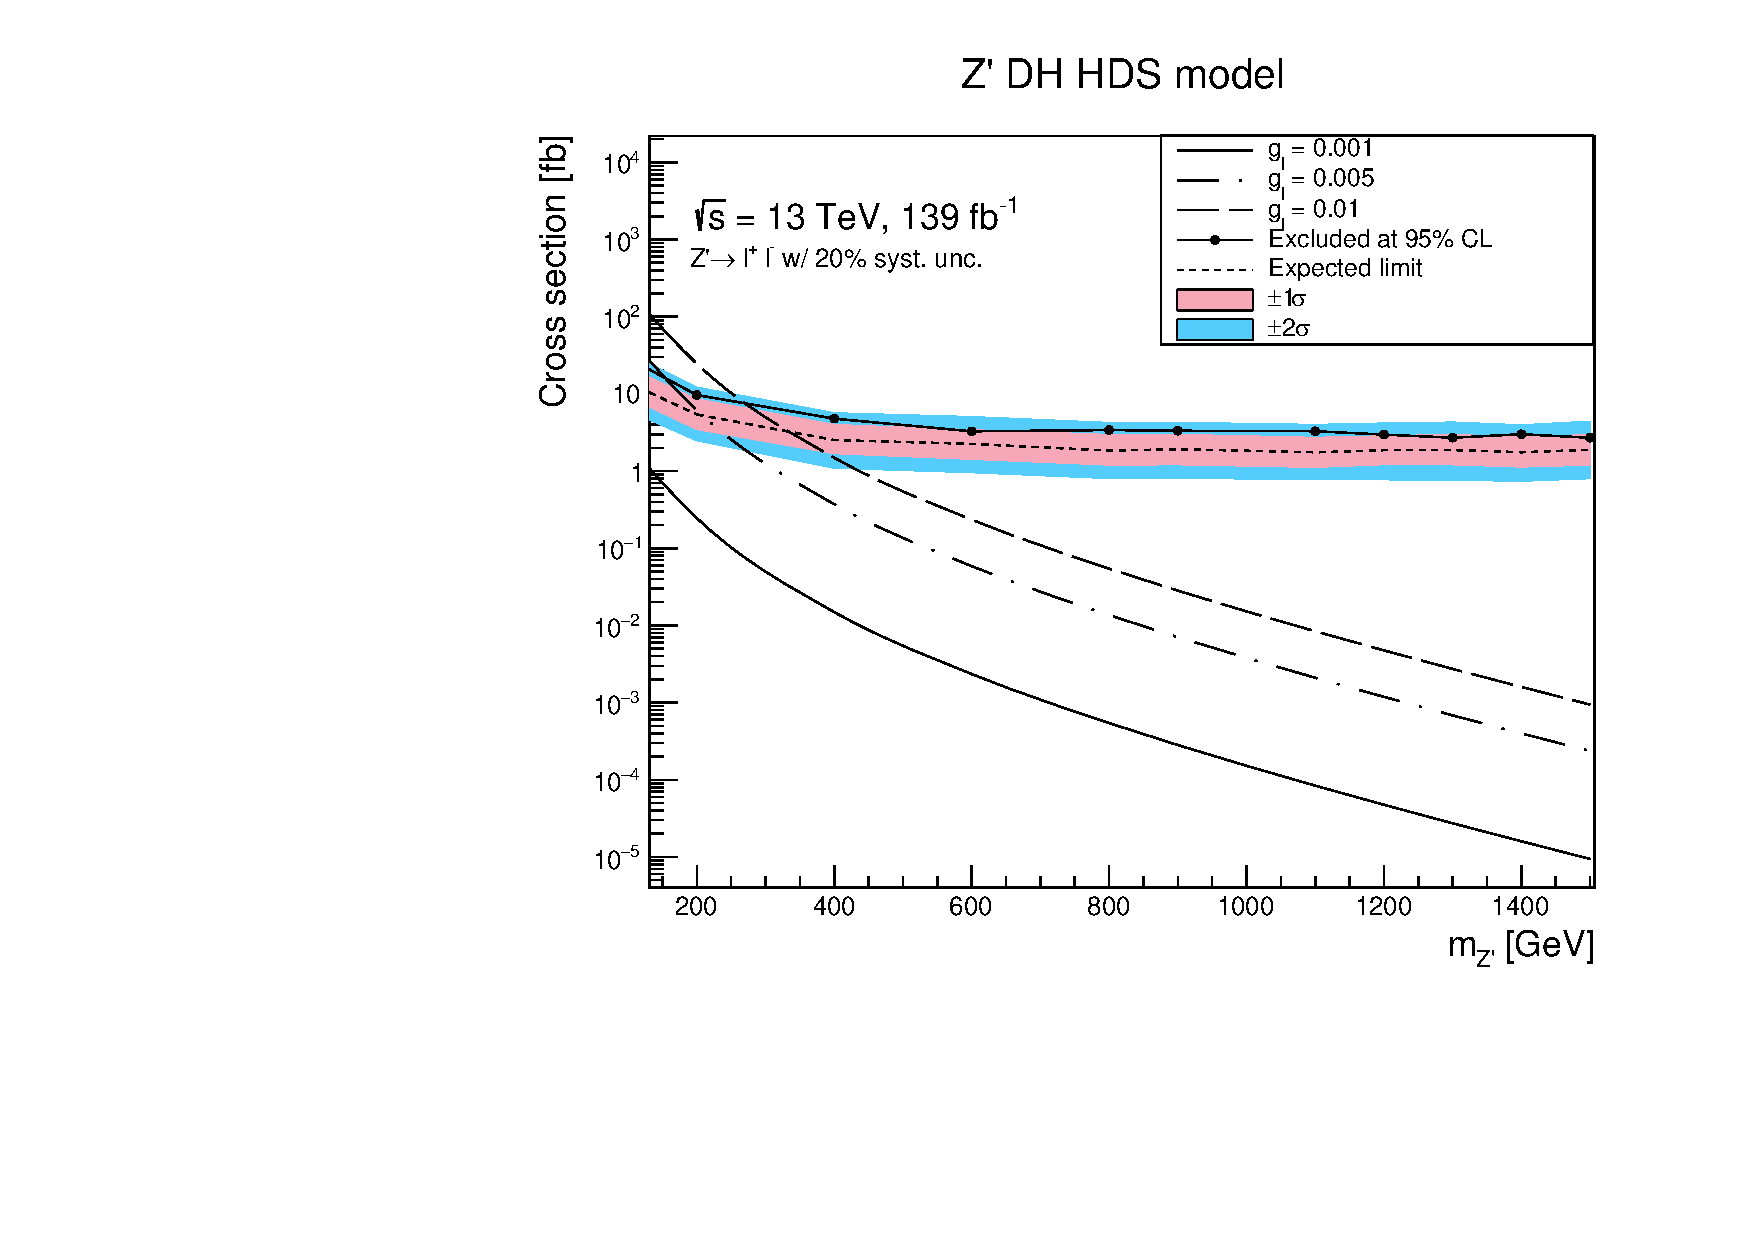
\includegraphics[width=1\textwidth]{Limits/DH_HDS/mass_exclusion_comb.pdf}
   \end{subfigure}
   \hfill
   \begin{subfigure}[b]{0.49\textwidth}
      \centering
      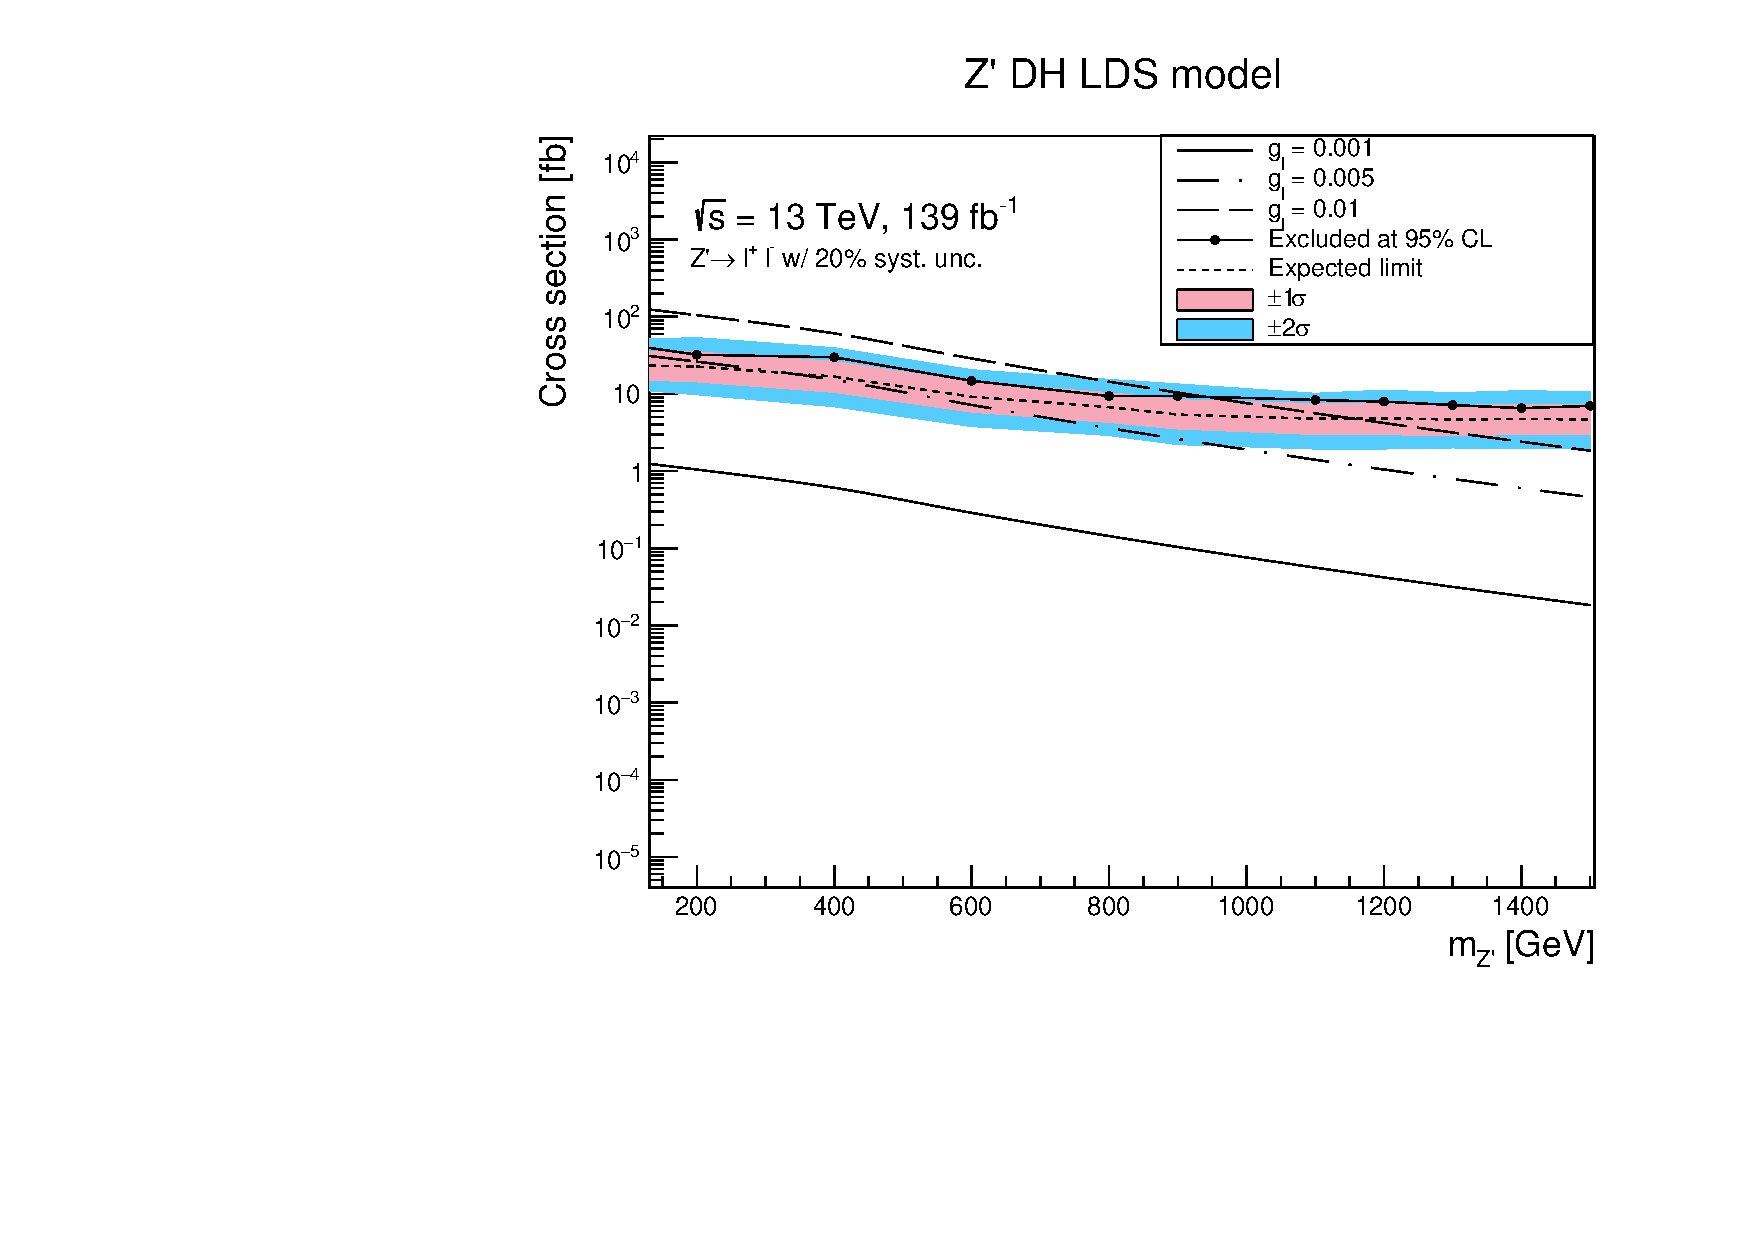
\includegraphics[width=1\textwidth]{Limits/DH_LDS/mass_exclusion_comb.pdf}
   \end{subfigure}
   \hfill
   \begin{subfigure}[b]{0.49\textwidth}
      \centering
      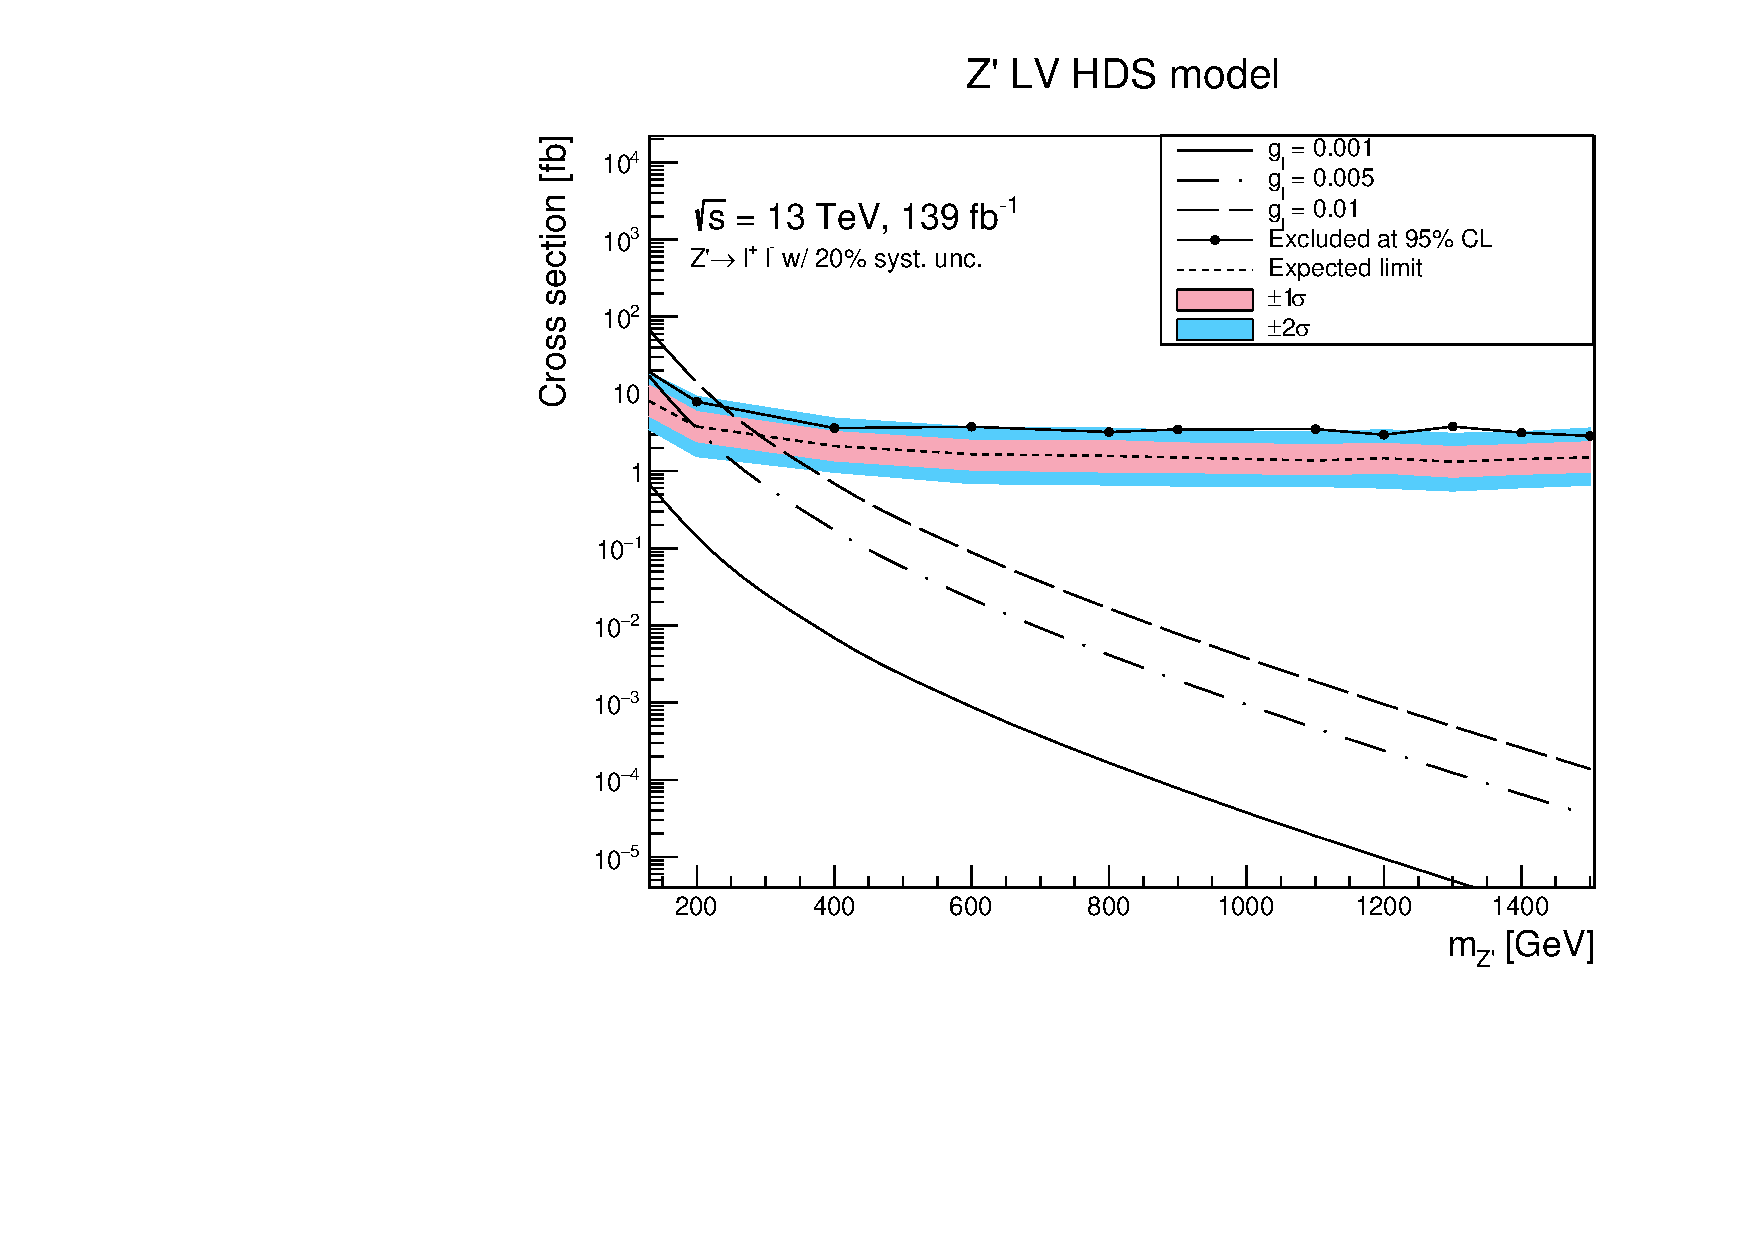
\includegraphics[width=1\textwidth]{Limits/LV_HDS/mass_exclusion_comb.pdf}
   \end{subfigure}
   \hfill
   \begin{subfigure}[b]{0.49\textwidth}
      \centering
      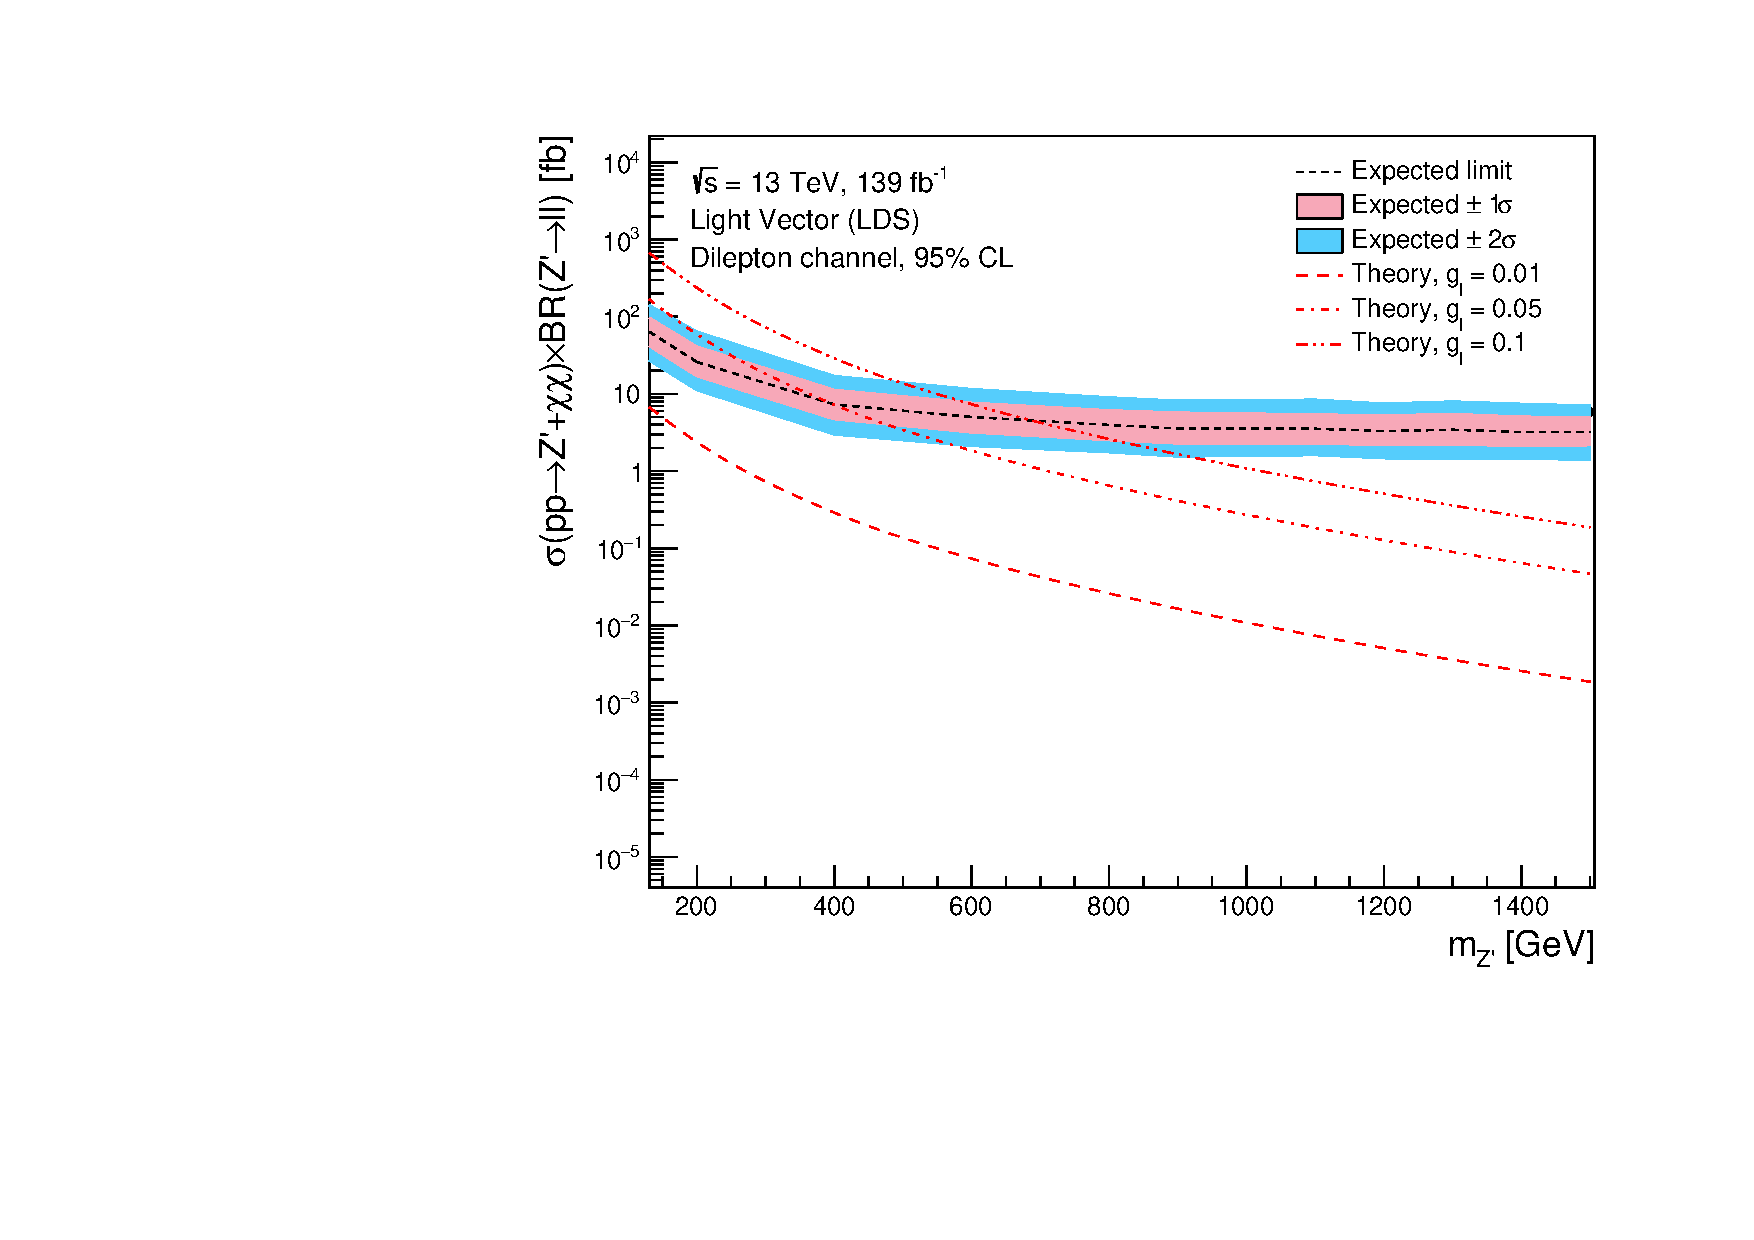
\includegraphics[width=1\textwidth]{Limits/LV_LDS/mass_exclusion_comb.pdf}
   \end{subfigure}
   \hfill
	\begin{subfigure}[b]{0.49\textwidth}
      \centering
      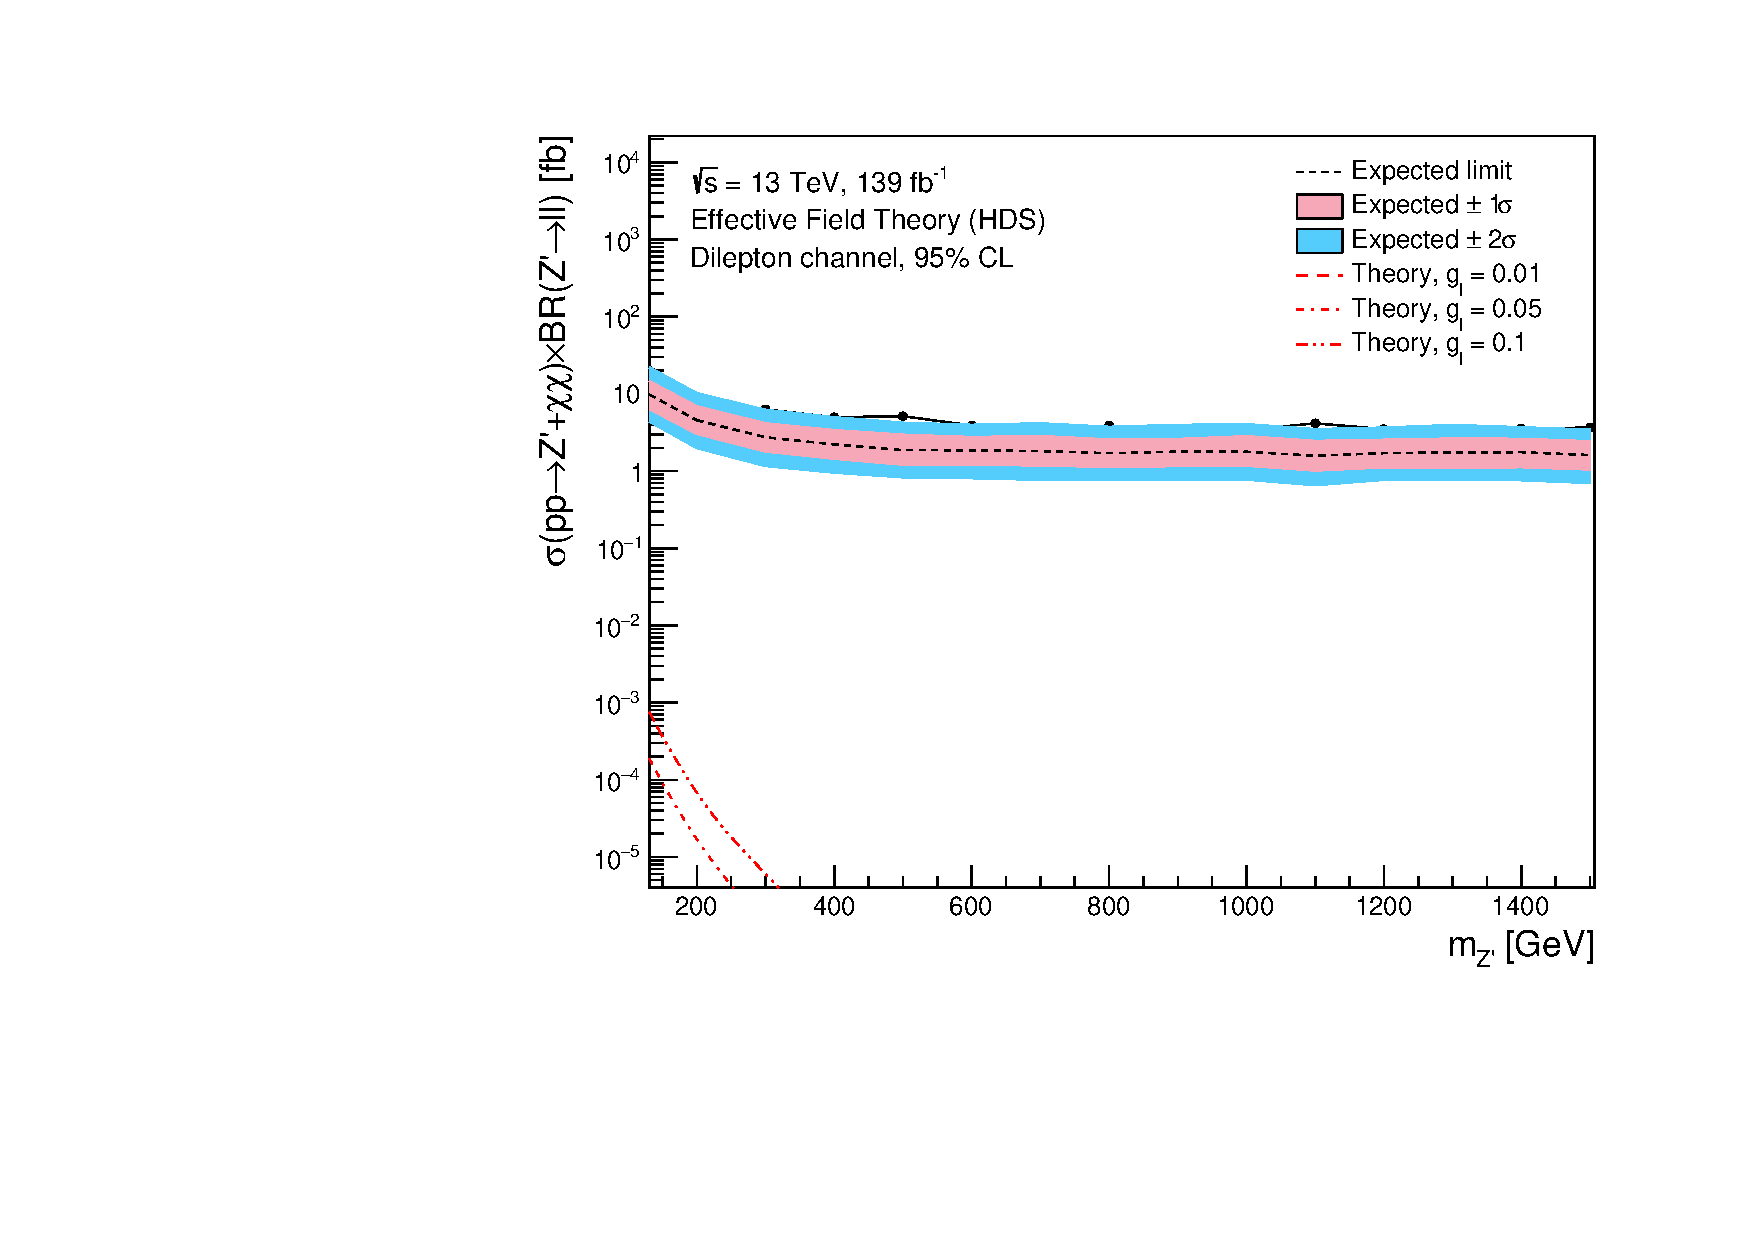
\includegraphics[width=1\textwidth]{Limits/EFT_HDS/mass_exclusion_comb.pdf}
   \end{subfigure}
   \hfill
   \begin{subfigure}[b]{0.49\textwidth}
      \centering
      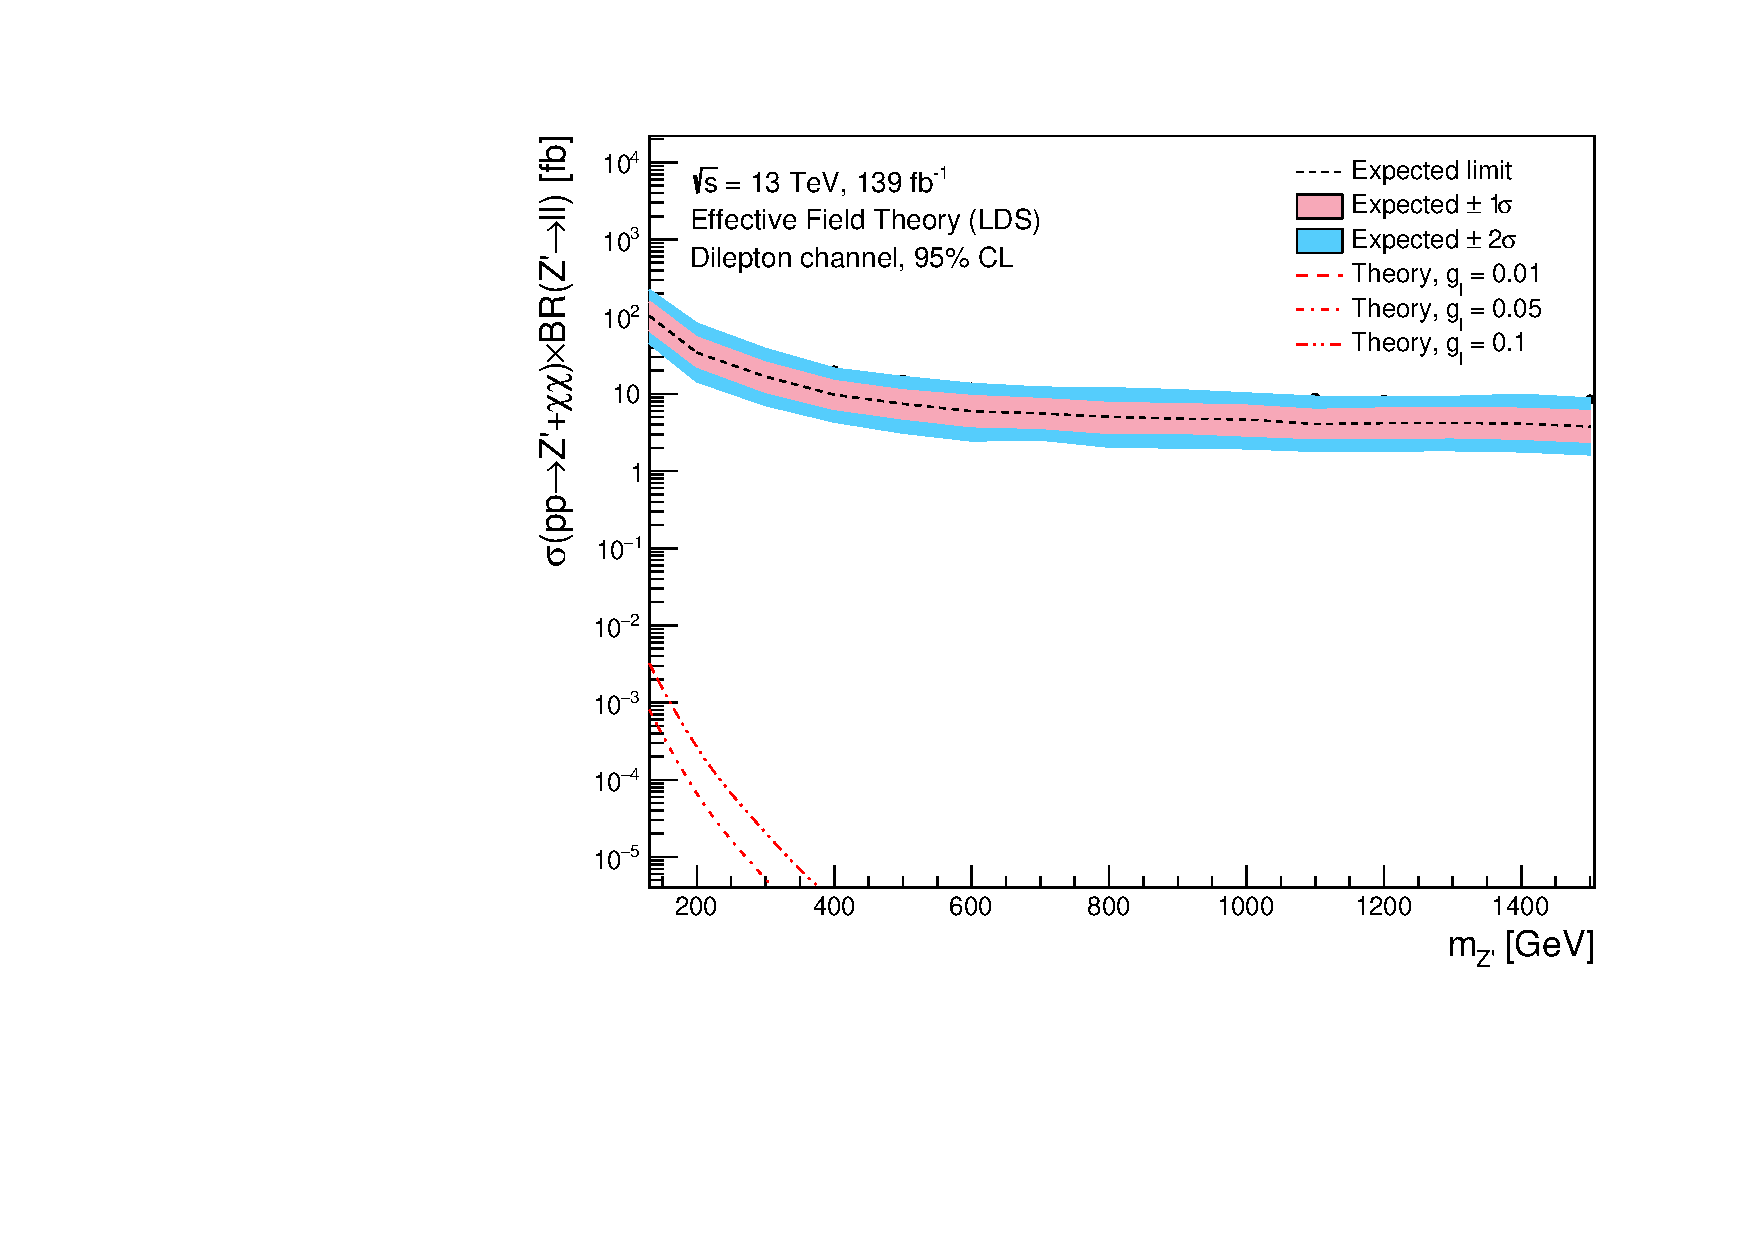
\includegraphics[width=1\textwidth]{Limits/EFT_LDS/mass_exclusion_comb.pdf}
   \end{subfigure}
   \caption[Mass exclusion limits of combined $ee$ and $\mu\mu$ channel for all mono-Z' models using the model dependent approach]{Mass exclusion limits of combined $ee$ and $\mu\mu$ channel for all mono-Z' models in both the Heavy Dark Sector (HDS) and Light Dark Sector (LDS) using the model dependent approach. 
   In the top row we have the mass exclusion of the Dark Higgs HDS (left) and Dark Higgs LDS (right) models. In the middle row we have the mass exclusions of the Light Vector HDS (left) and Light Vector LDS (right) models. In the bottom row we have the mass exclusion of the 
   inelastic EFT HDS (left) and inelastic EFT LDS (right) models.
   The y-axis on all plots represents the cross-section times branching ratio of the process we are studying. The x-axis is the mass of the $Z'$ boson. We did not interpolate between the available masses we had simulated, 
   and have rather just connected the values calculated for each mass point by connecting the points. The dashed black line is the expected 95\% CL limit calculated using Bayesian statistics with a 1$\sigma$ and 2$\sigma$ deviation. 
   The different dashed lines represent the theoretical cross-section times branching ratio of the process when varying the value of the lepton coupling $g_l$ between the leptons and the $Z'$ boson. The simulated events in this thesis utilized the value $g_l=$ 0.01, we include the cross-section times branching ratio when increasing this coupling to 0.05 and 0.1 to see how the exclusions change. 
   }\label{fig:model_dep_mono_Zp_excl}
\end{figure}



\clearpage
\section{Model independent approach}
The second method we utilized in this analysis was to train three BDTs in different orthogonal Signal Regions (SR) of kinematical phase space using a dataset that included all the available DM models with a dilepton and Missing Transverse Energy (MET) final state. The DM models we studied were a supersymmetric direct slepton production model, a Two Higgs Doublet Model with an additional pseudoscalar $a$ 
(2HDM + a), and three mono-$Z'$ models, Dark Higgs (DH), Light Vector (LV) and inelastic EFT. The three mono-$Z'$ models were furthermore divided into a Heavy Dark Sector (HDS) and a Light Dark Sector (LDS). As this method uses models that share similar experimental features, like the final state, 
but are based of different theoretical principles, we called this method for the model independent approach. The three SR we chose to divide the dataset in were 
\begin{itemize}
   \item SR1: $m_{ll} >110$ GeV and $E_T^{miss} \in [50, 100]$ GeV
   \item SR2: $m_{ll} >110$ GeV and $E_T^{miss} \in [100, 150]$ GeV
   \item SR3: $m_{ll} >110$ GeV and $E_T^{miss} >150$ GeV,
\end{itemize}
where the invariant mass cut $m_{ll}>110$ GeV was chosen to remove the Z-boson peak.\\
\\To not repeat how we arrive at the expected mass exclusion limits, which was discussed in detail in Section \ref{sec:Walkthrough}, we will present how this method was used by looking at the expected mass exclusion limit when testing on the DH HDS model. 
As the SRs we chose are orthogonal in MET we assume that they are not correlated, meaning that we can statistically combine the results for each SR to get a combined mass exclusion limit in a combined SR. This is shown in Figure \ref{fig:DH_HDS_me_SRS} where we can see how the mass exclusion looks for
the electron channel in every SR, including the combined SR limit. \\
\begin{figure}[!ht]
	\centering
	\begin{subfigure}[b]{0.49\textwidth}
      \centering
      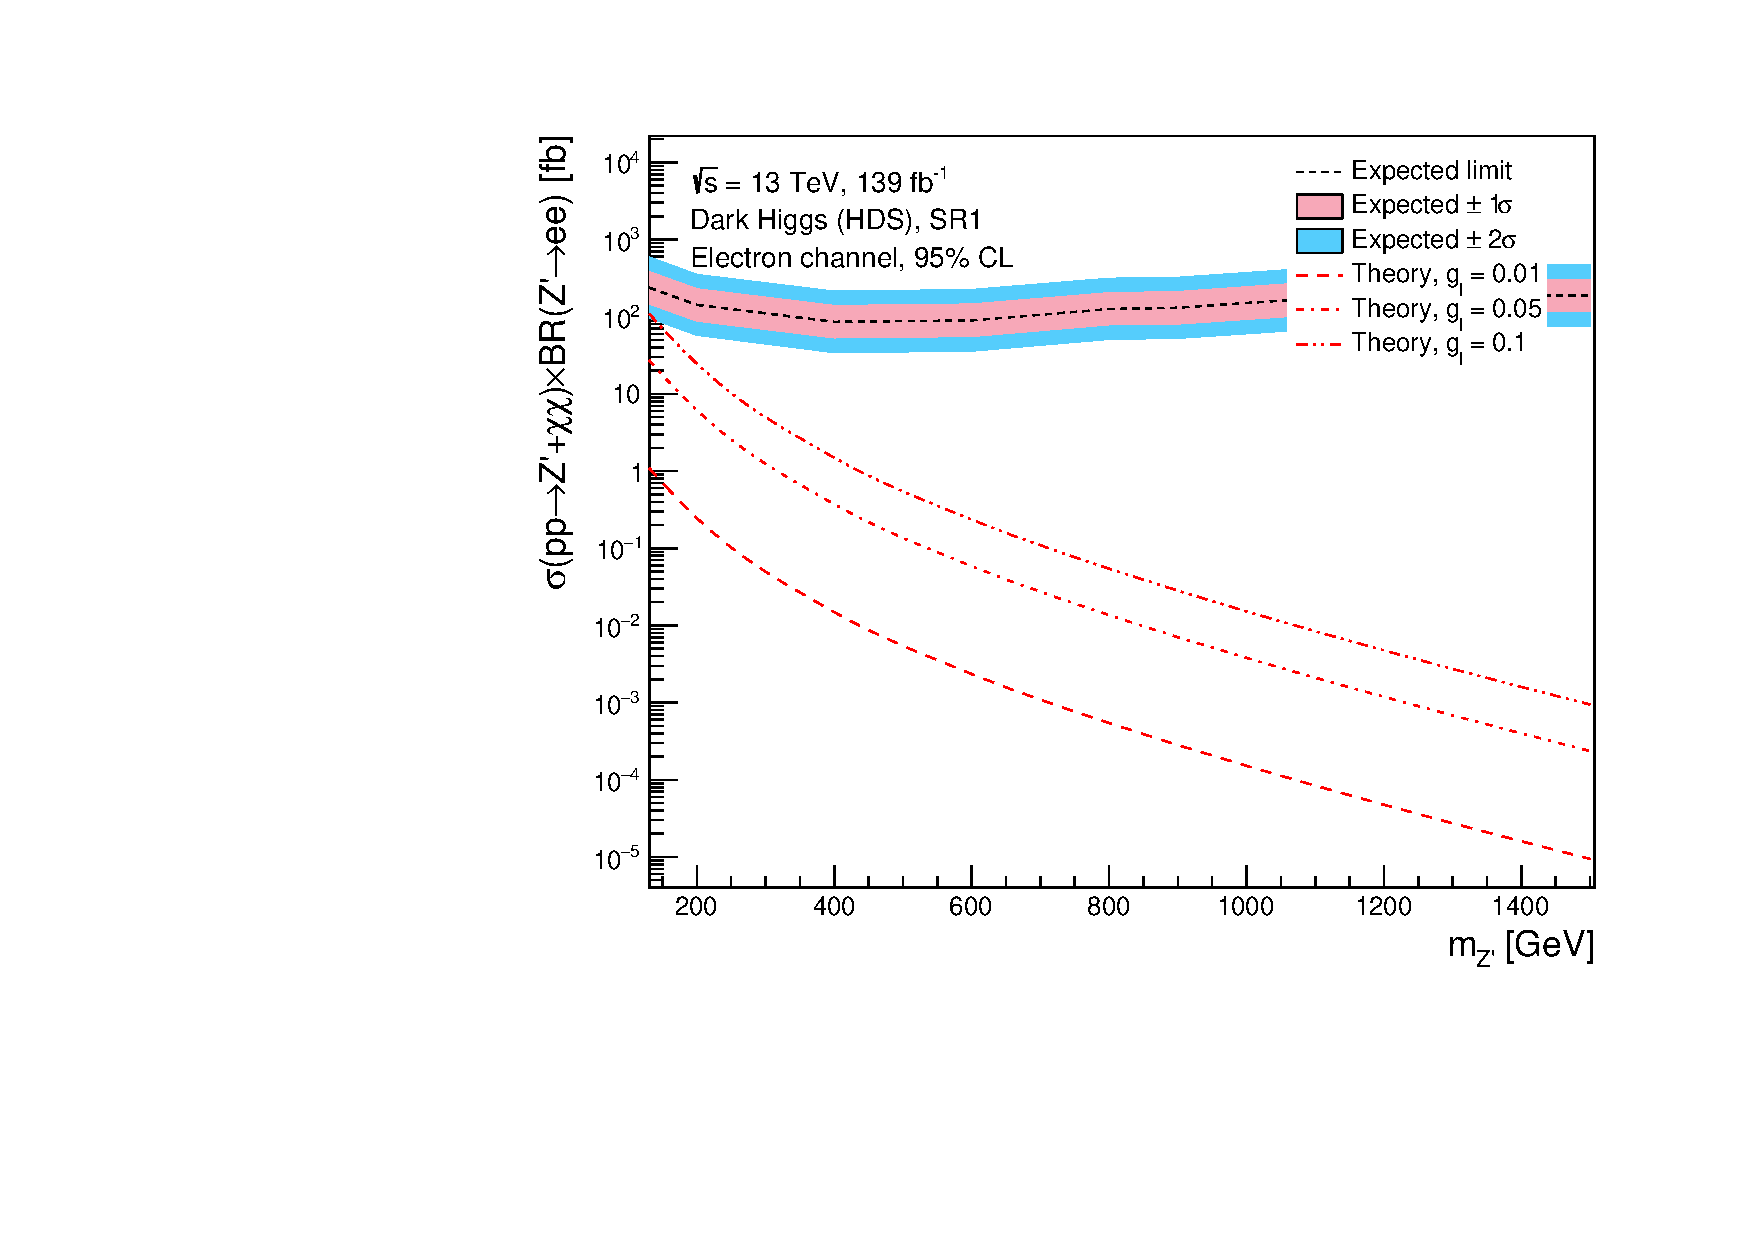
\includegraphics[width=1\textwidth]{Limits/Model_independent/50-100/DH_HDS/mass_exclusion_ee.pdf}
   \end{subfigure}
   \hfill
   \begin{subfigure}[b]{0.49\textwidth}
      \centering
      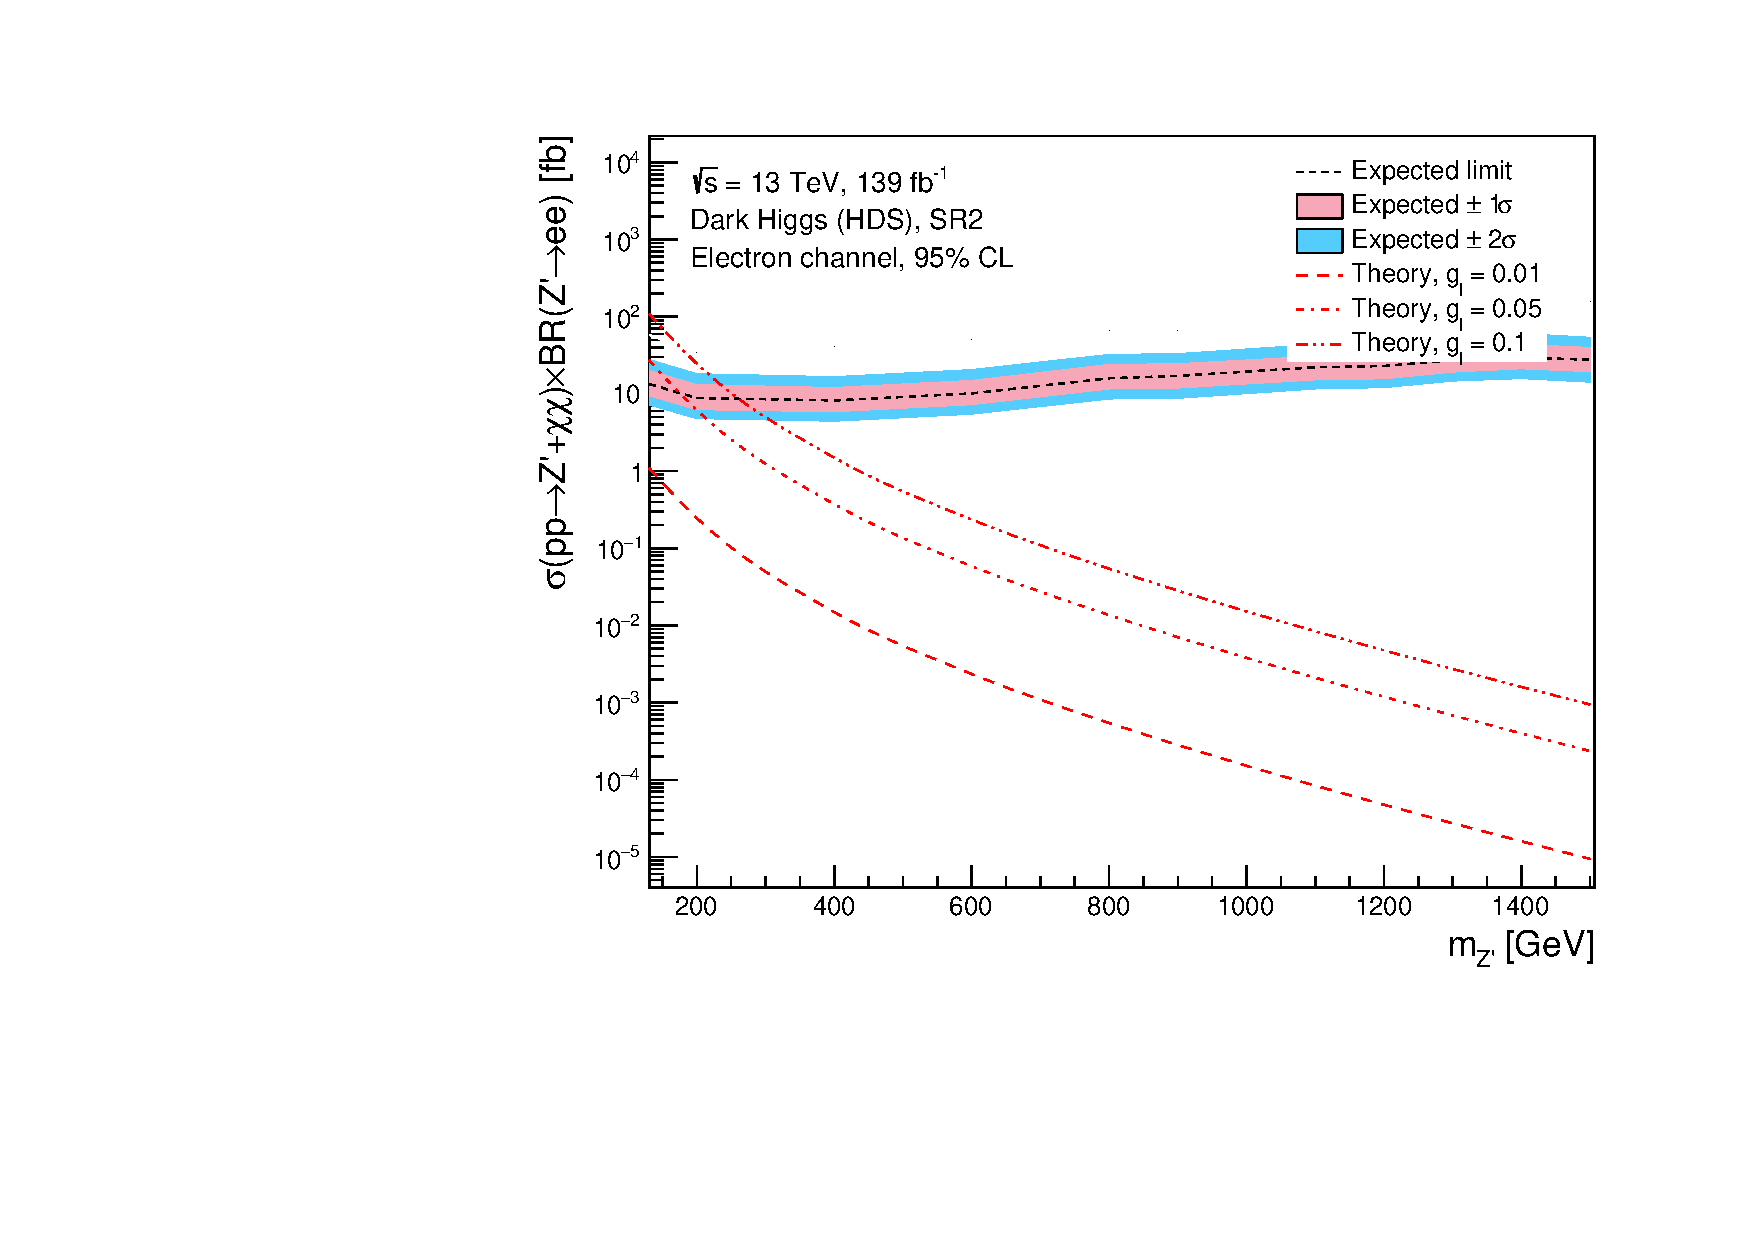
\includegraphics[width=1\textwidth]{Limits/Model_independent/100-150/DH_HDS/mass_exclusion_ee.pdf}
   \end{subfigure}
   \hfill
	\begin{subfigure}[b]{0.49\textwidth}
      \centering
      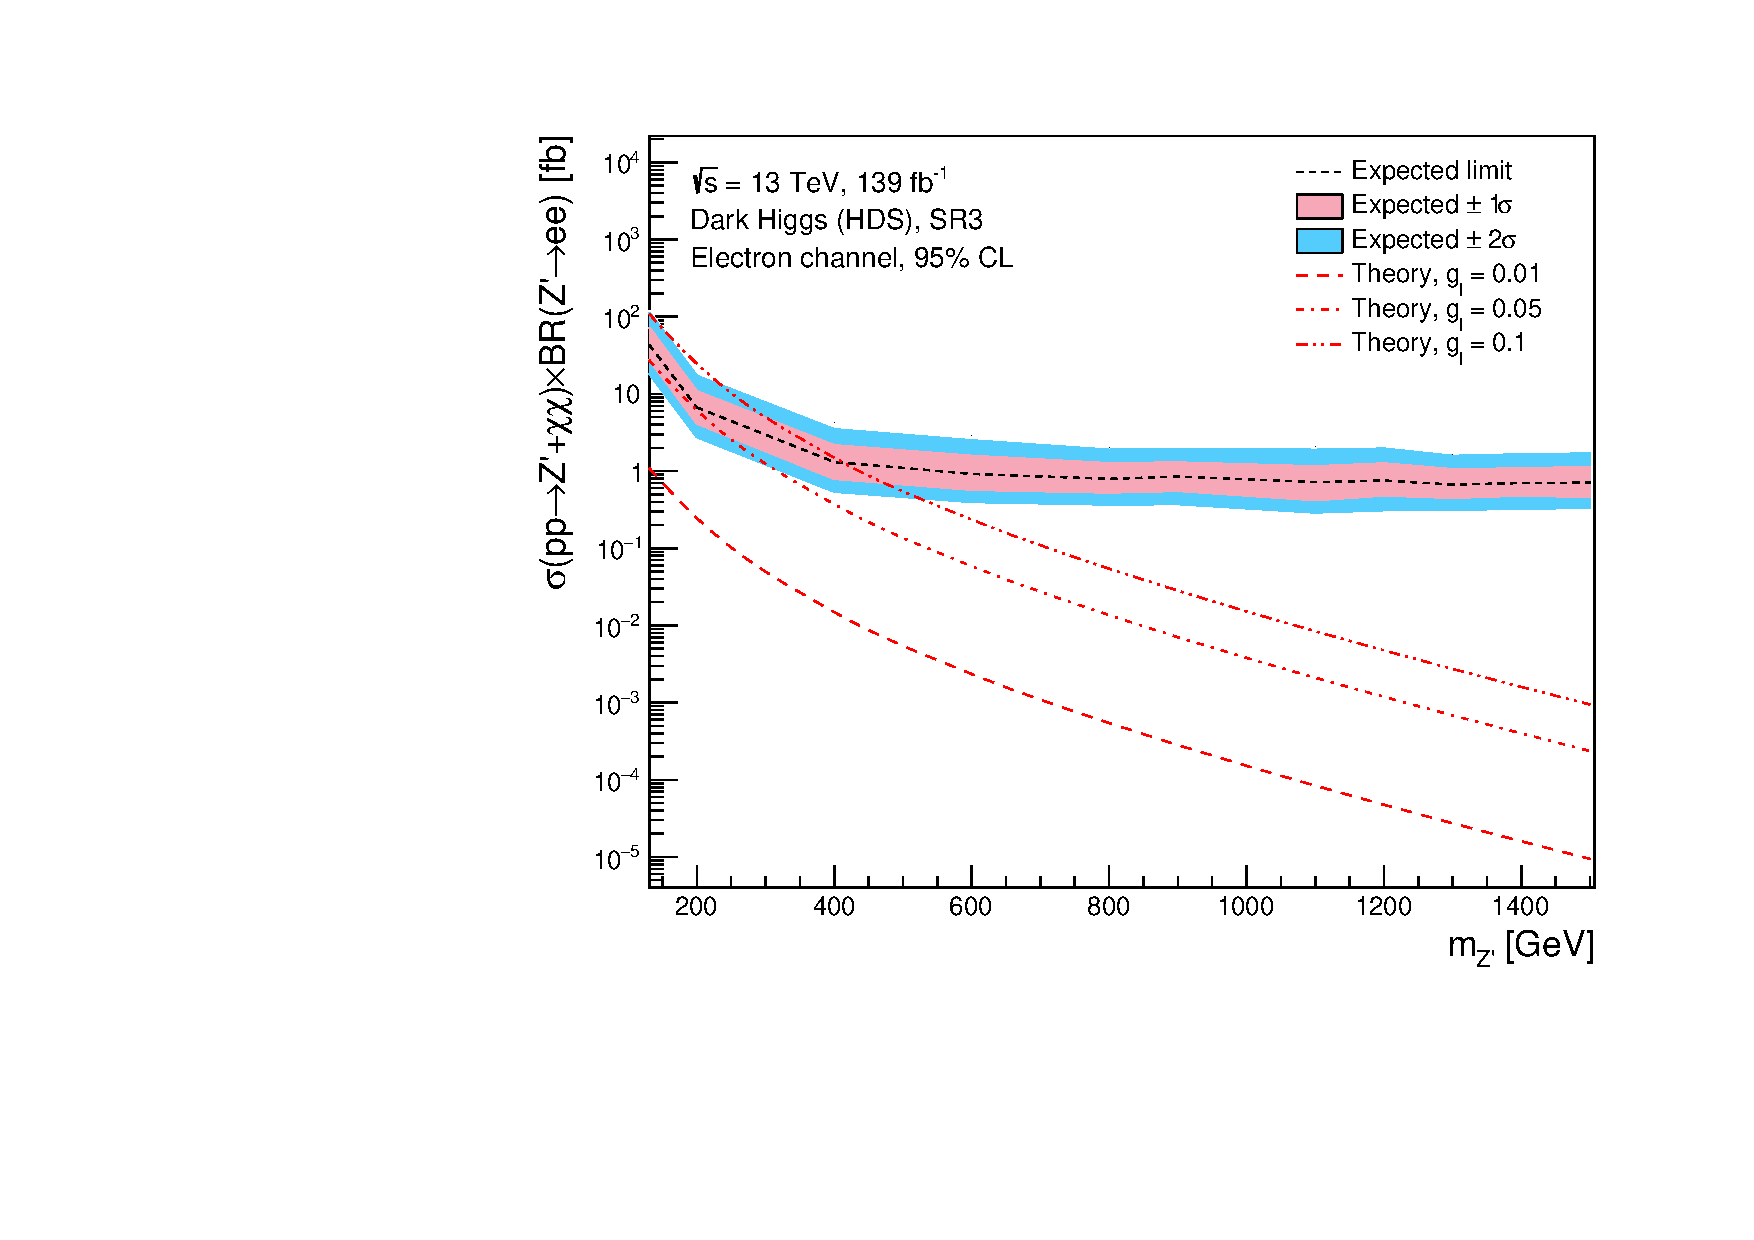
\includegraphics[width=1\textwidth]{Limits/Model_independent/150/DH_HDS/mass_exclusion_ee.pdf}
   \end{subfigure}
   \hfil
   \begin{subfigure}[b]{0.49\textwidth}
      \centering
      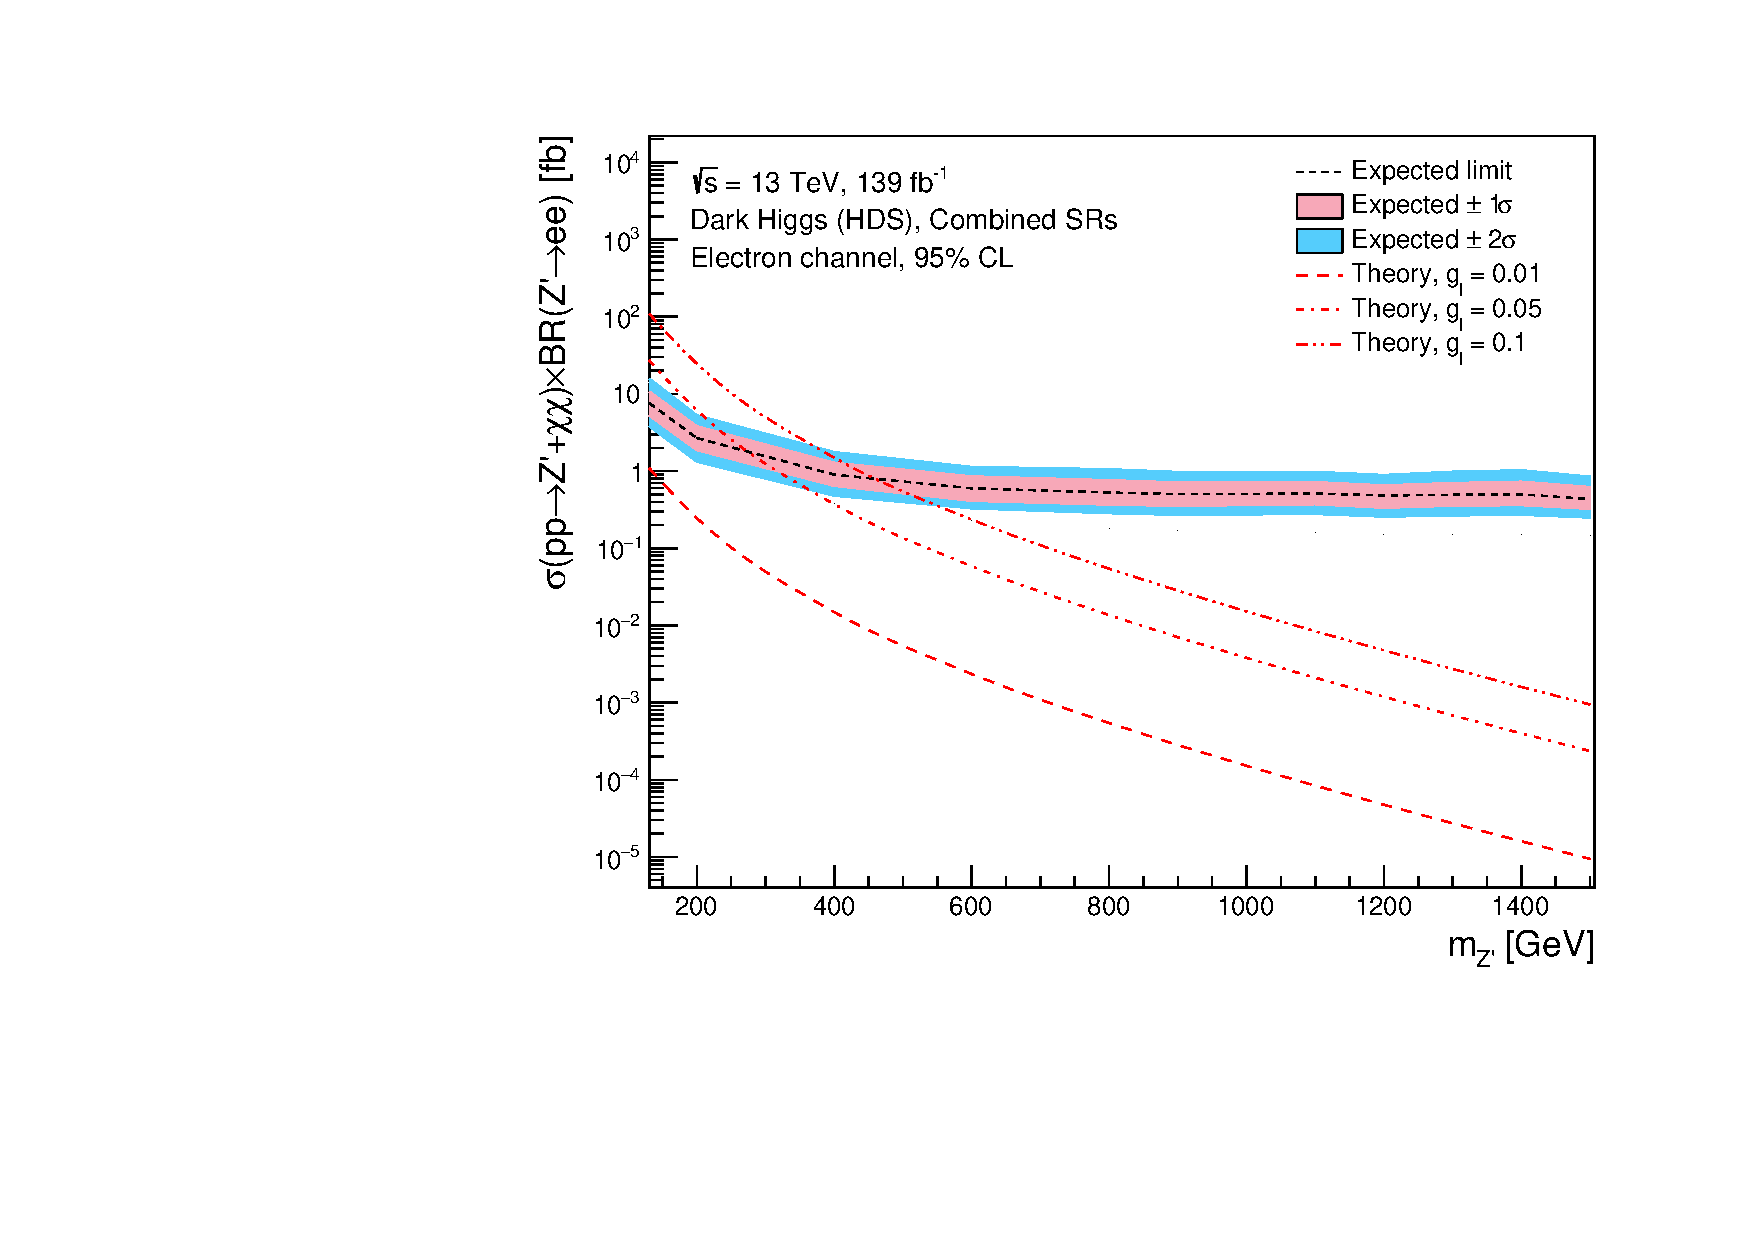
\includegraphics[width=1\textwidth]{Limits/Model_independent/DH_HDS/mass_exclusion_ee.pdf}
   \end{subfigure}
   \caption[Electron channel mass exclusions in DH HDS using the model independent approach]{Mass exclusion limits results for Dark Higgs Heavy Dark Sector model on the $ee$ channel in all SRs, including the combined SR channel. All SRs used in this thesis had $m_{ll}>110$ GeV.
   In the top left we have the expected mass exclusion in SR1 where $E_T^{miss} \in [50, 100]$ GeV. In the top right we have the expected mass exclusion in SR2 where $E_T^{miss} \in [100, 150]$ GeV. In the bottom left we have the expected mass exclusion limit in SR3 where $E_T^{miss} >150$ GeV. 
   In the bottom right we have the expected mass limit for the model when statistically combining the result of SR1, SR2 and SR3. 
   The y-axis on all plots represents the cross-section times branching ratio of the process we are studying. The x-axis is the mass of the $Z'$ boson. We did not interpolate between the available masses we had simulated, 
   and have rather just connected the values calculated for each mass point by connecting the points. The dashed black line is the expected 95\% CL limit with a 1$\sigma$ and 2$\sigma$ deviation. 
   The different dashed lines represent the theoretical cross-section times branching ratio of the process when varying the value of the lepton coupling $g_l$ between the leptons and the $Z'$ boson. The simulated events in this thesis utilized the value $g_l=$ 0.01, we include the cross-section times branching ratio when increasing this coupling to 0.05 and 0.1 to see how the exclusions change. }\label{fig:DH_HDS_me_SRS}
\end{figure} 
\\In Figure \ref{fig:DH_HDS_me_SRS} we can see that we can not exclude anything in SR1 (top left plot), we also see that as we go to SR2 (top right plot) the exclusion gets better, and we can exclude the model up to $m_{Z'}\approx250$ GeV when we set $g_l=0.1$\footnote{See Section \ref{sec:Walkthrough} for discussion on lepton coupling variations with the mono-$Z'$ models.}. 
This exclusion gets higher when we go to SR3 (bottom left plot), where we can exclude the model up to $m_{Z'}\approx425$ GeV when setting $g_l=0.1$, but the expected limit is slightly lower than for SR2. However, when statistically combining the results for every SR (bottom right plot) we now get that we can exclude the model up to $m_{Z'}\approx450$ GeV with $g_l=0.1$,
while having an overall lower expected limit with smaller 1$\sigma$ and 2$\sigma$ deviations. This means that this method of dividing into several SRs yields higher exlcusions. \textbf{Question: Should I state already that this is better than the model dependent approach or should I keep this for the next section?}\\
\\ This can be generalized for every model studied, the exclusion limits for the dilepton channel and combined SRs for the other direct slepton production and 2HDM + a model can be seen in Figure \ref{fig:model_indep_excl}, and in Figure \ref{fig:model_indep_mono_Zp_excl} for the mono-$Z'$ models.
To see all the plots used to arrive at these limits for every model you can see the GitHub repo\footnote{Available here: \href{https://github.com/rubenguevara/Master-Thesis/tree/master/Plots/XGBoost/Model_independent}{https://github.com/rubenguevara/Master-Thesis/tree/master/Plots\\/XGBoost/Model\_independent}}, 
and to see all the tables with inputs see Appendix \ref{chap:Limit_Tabs}.
\begin{figure}[!ht]
	\centering
	\begin{subfigure}[b]{0.49\textwidth}
      \centering
      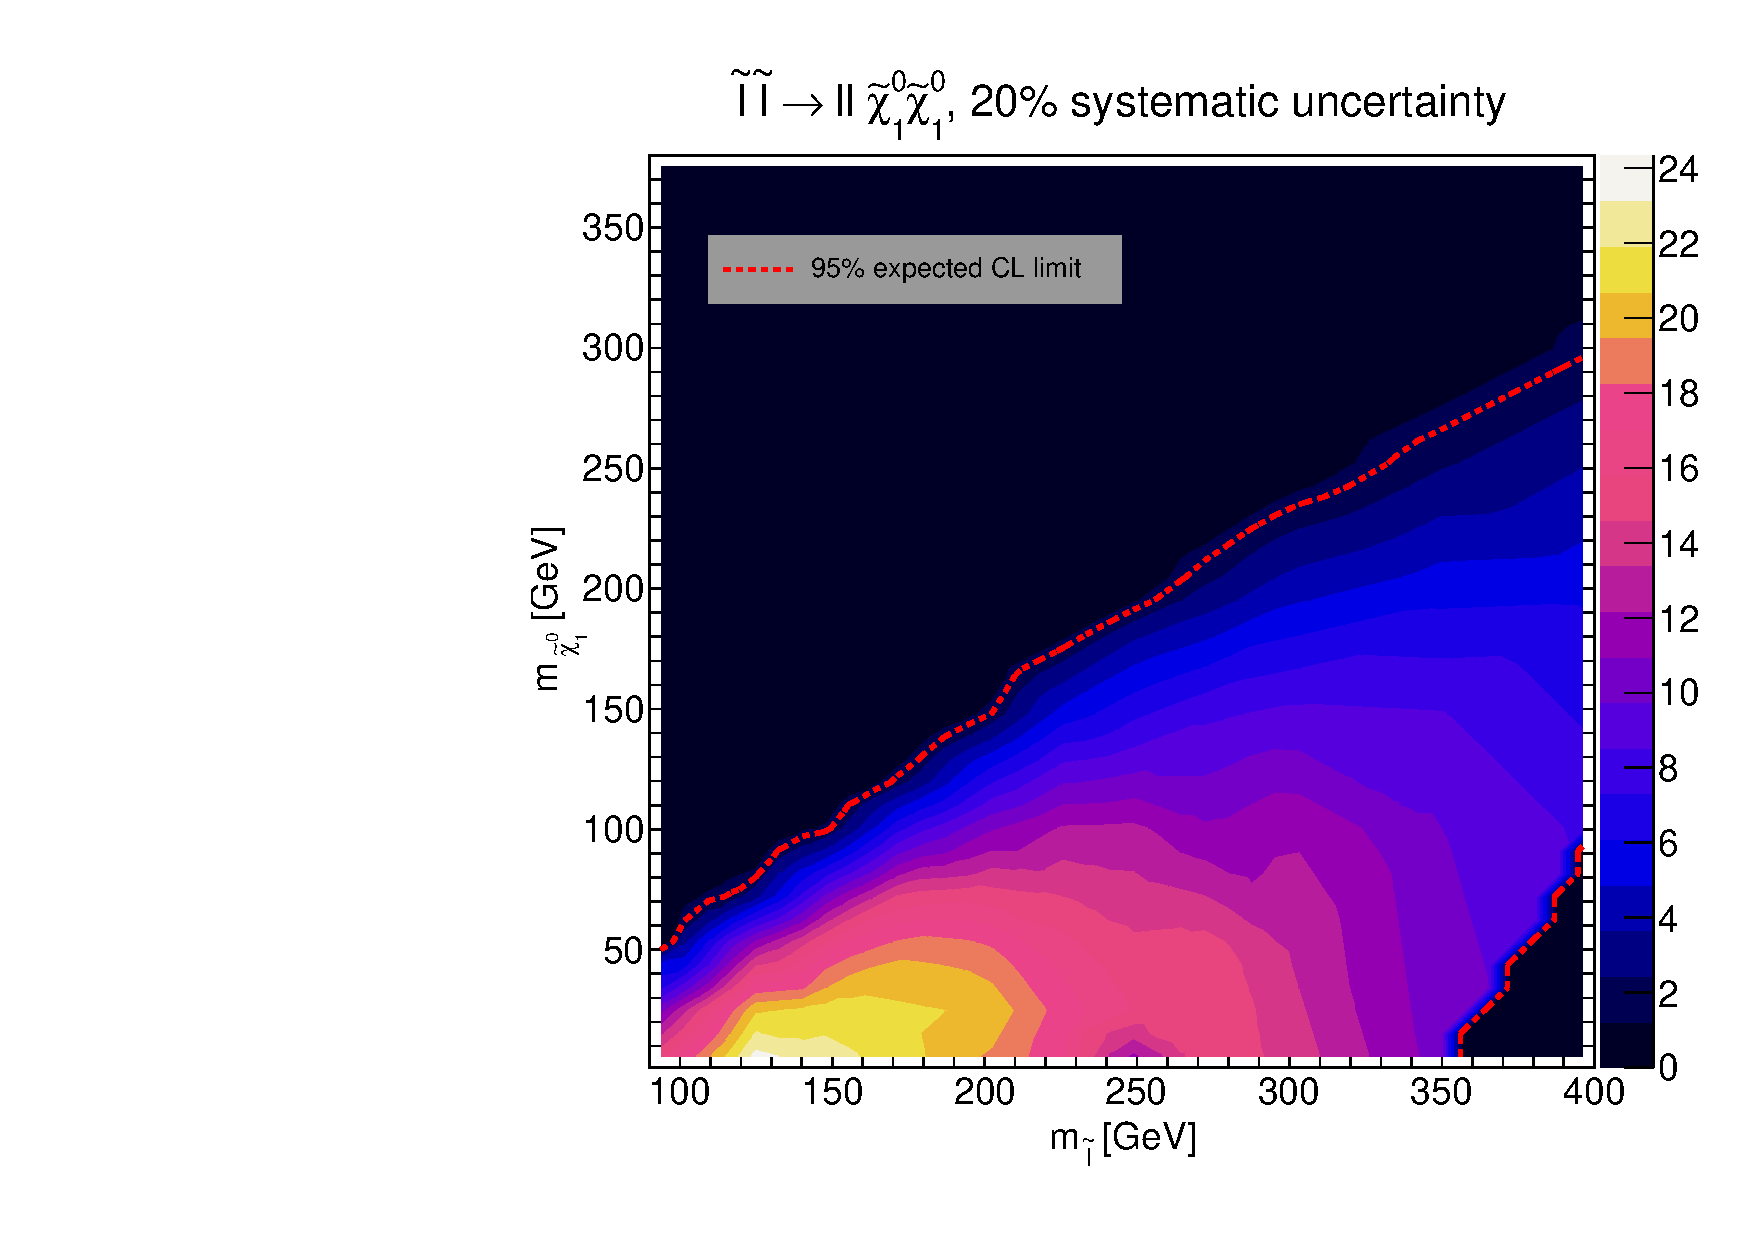
\includegraphics[width=1\textwidth]{Limits/Model_independent/SlepSlep/SlepSlep_ll.pdf}
   \end{subfigure}
   \hfill
   \begin{subfigure}[b]{0.49\textwidth}
      \centering
      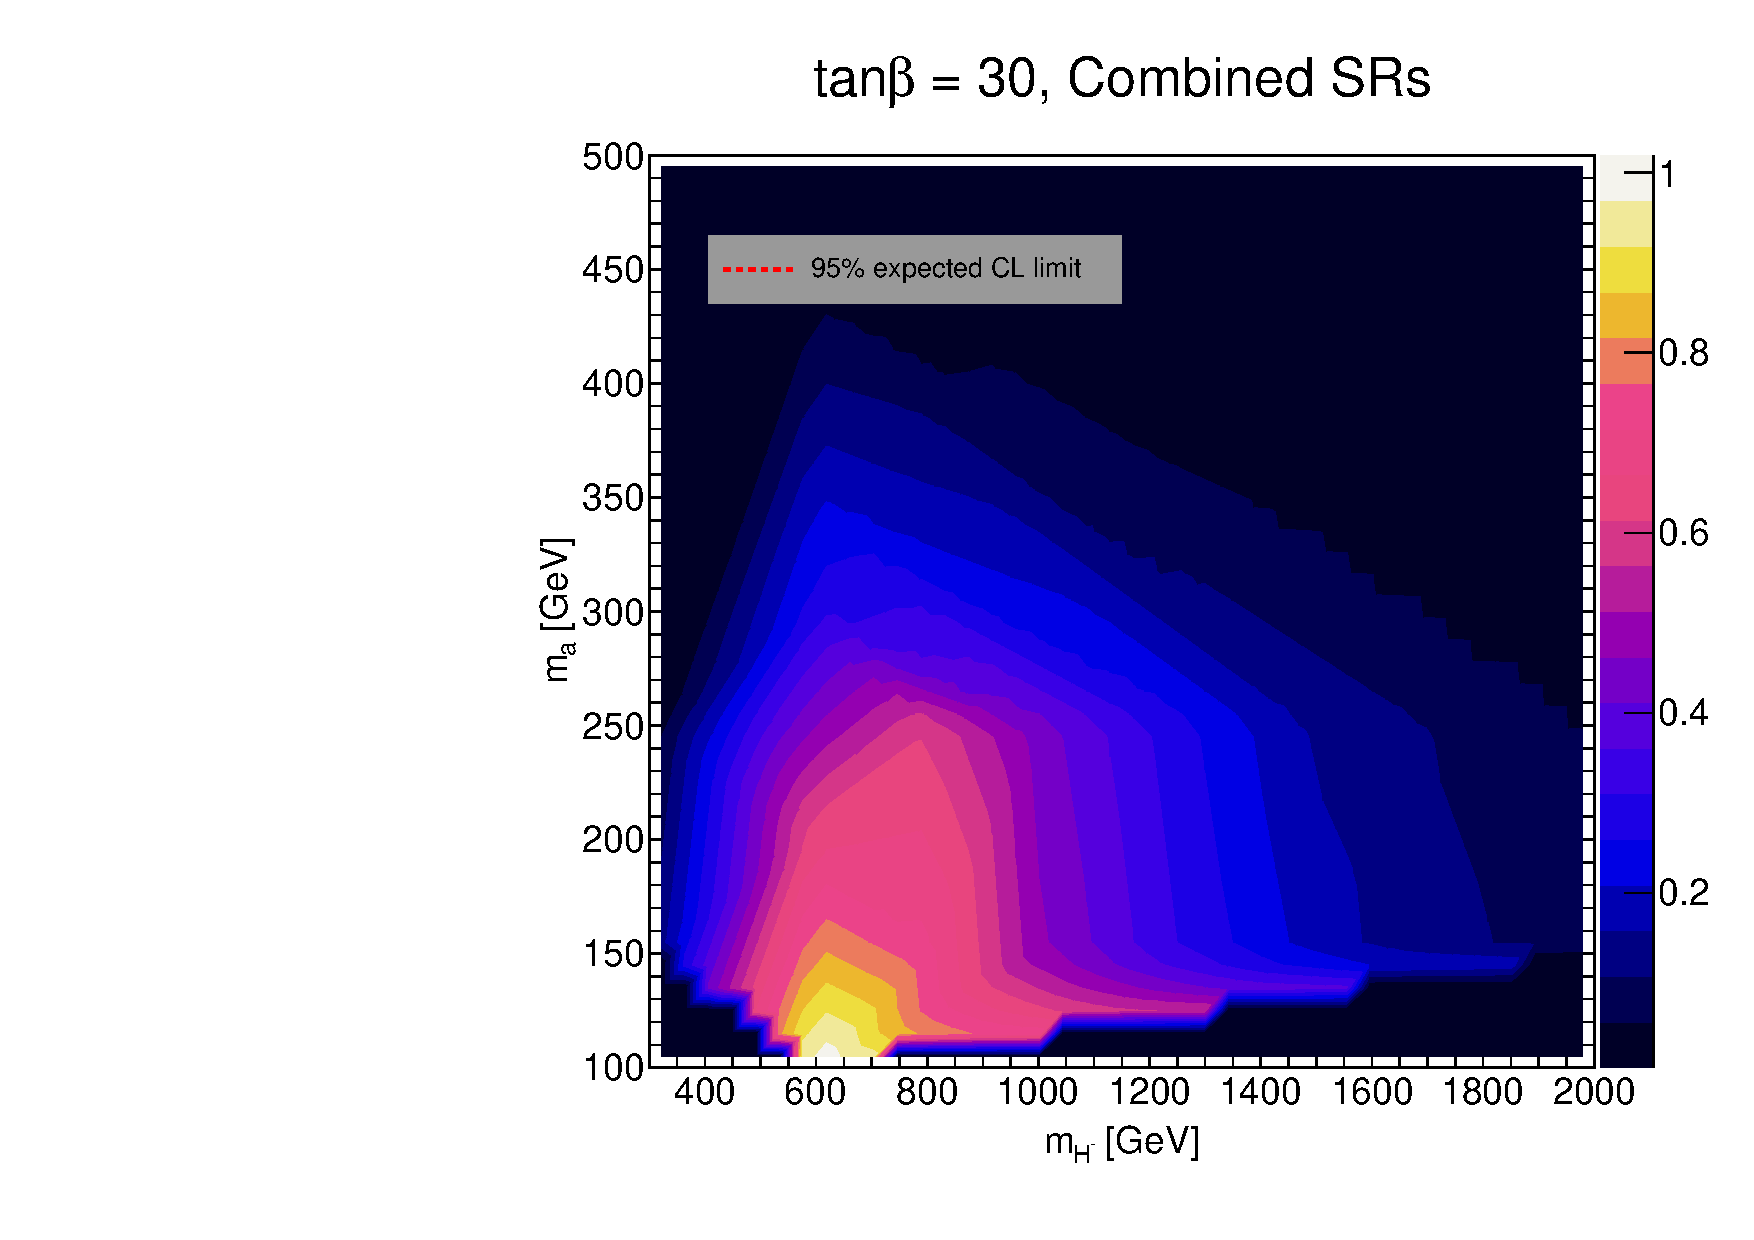
\includegraphics[width=1\textwidth]{Limits/Model_independent/2HDM/2HDM_ll_tb30.pdf}
   \end{subfigure}
   \caption[Mass exclusion limits of combined $ee$ and $\mu\mu$ channel for direct slepton production and 2HDM + a using the model independent approach]{
      Mass exclusion limits of combined $ee$ and $\mu\mu$ channel for direct slepton production (left) and 2HDM + a for $\tan\beta=30$ (right) using the model independent approach. The plots here have the two varying masses as the axes, the z-axis is the expected significance calculated using Eq. (\ref{eq:significance}) with uncertainties. The expected 95\% CL limit was chosen using Frequentist statistics using the significance $Z=$ 1.645.   
      For the direct slepton production model we have the slepton mass, $m_{\tilde{\ell}}$, on the x-axis, and the neutralino mass on $m_{\tilde{\chi}_1^0}$ the y-axis. 
      For the 2HDM + a model we have the charged Higgs mass, $m_{H^-}$, on the x-axis, and the pseudoscalar $a$ mass $m_{a}$ on the y-axis. To see the exclusions for the other values of $\tan\beta$ on the 2HDM + a model see Appendix \ref{apx:MDA}. 
      Something to note about the direct slepton production plot (left), is the lack of exclusions in the bottom right corner where $m_{\tilde{\ell}}>350$ GeV and $m_{\tilde{\chi}_1^0}<50$ GeV, the reason for this is because we did not have any simulated event at that mass range, 
      to see the samples we had available see Figure \ref{fig:slepslep_mass}.
      }\label{fig:model_indep_excl}
\end{figure}
\begin{figure}[!ht]
	\centering
	\begin{subfigure}[b]{0.49\textwidth}
      \centering
      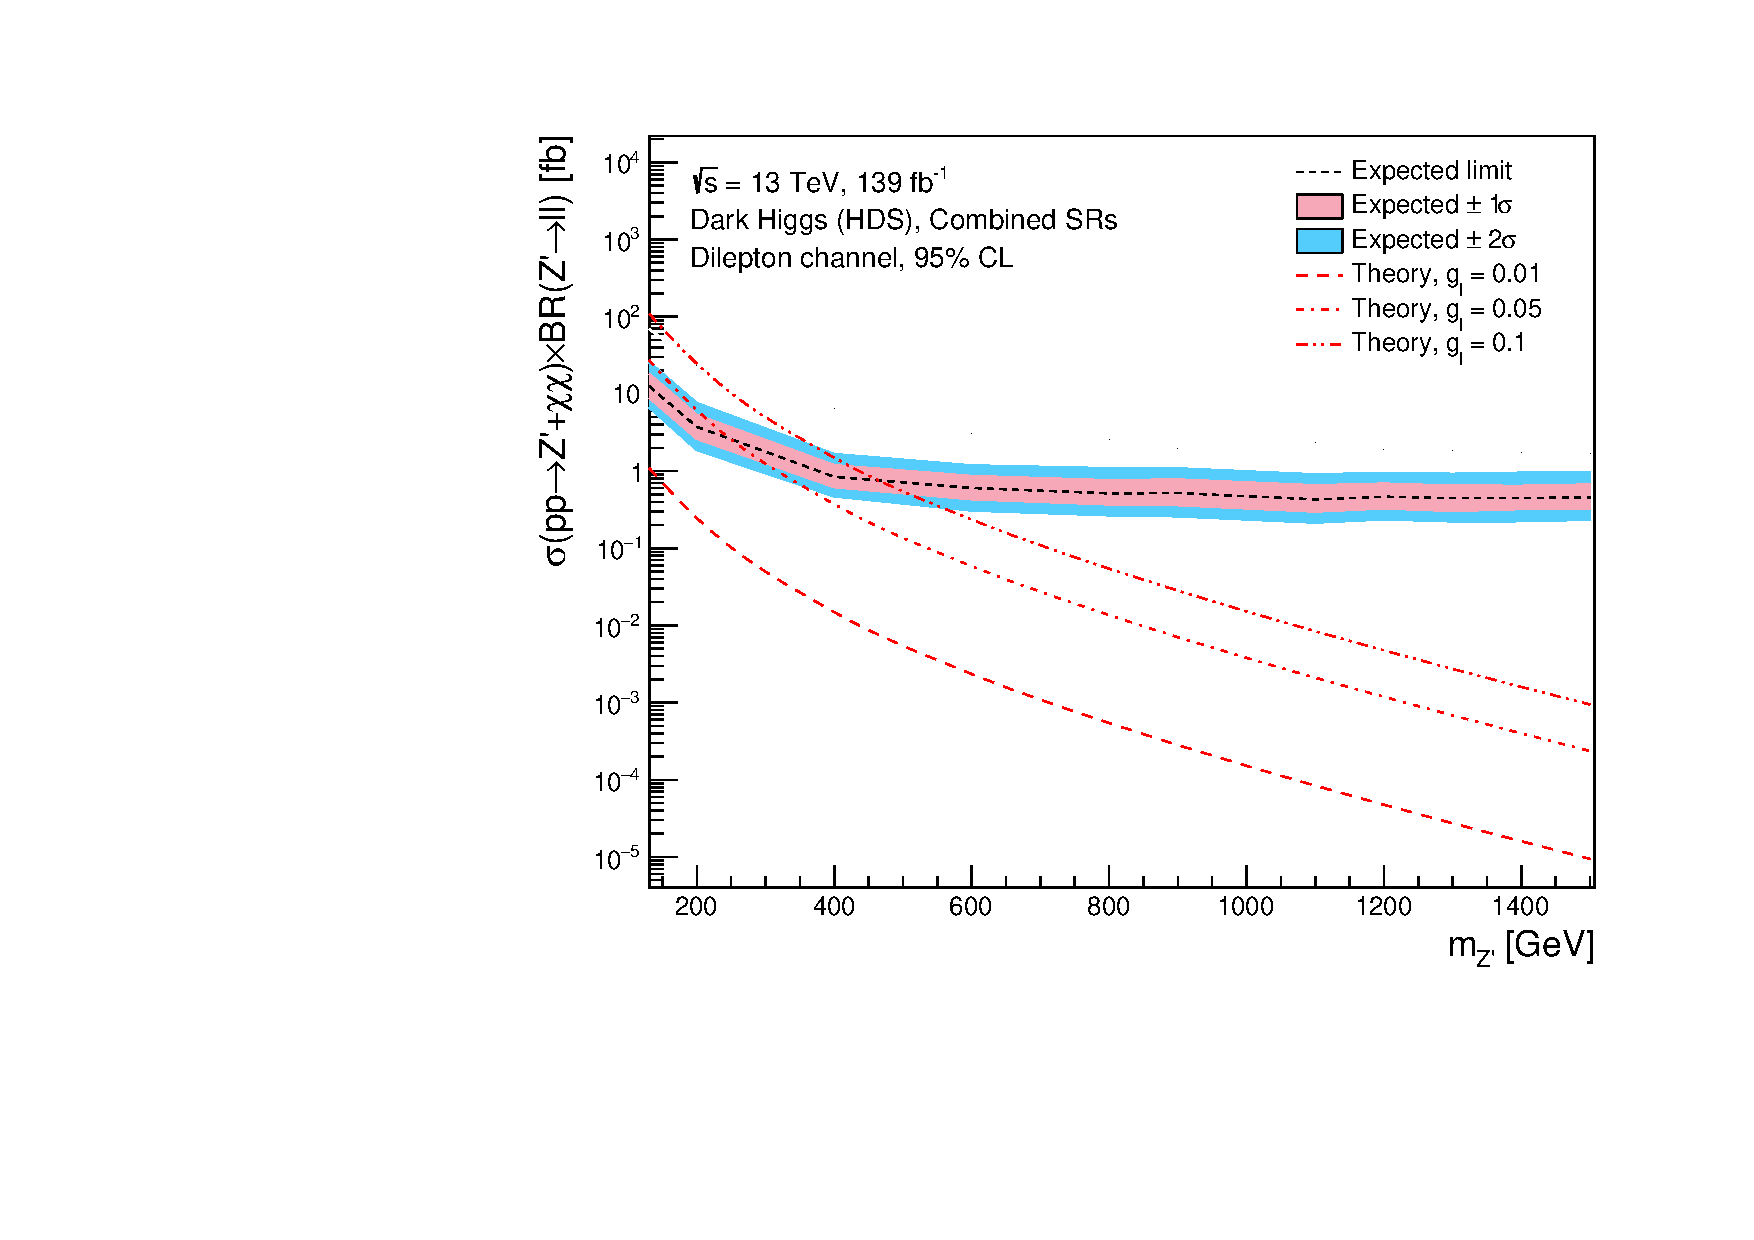
\includegraphics[width=1\textwidth]{Limits/Model_independent/DH_HDS/mass_exclusion_comb.pdf}
   \end{subfigure}
   \hfill
   \begin{subfigure}[b]{0.49\textwidth}
      \centering
      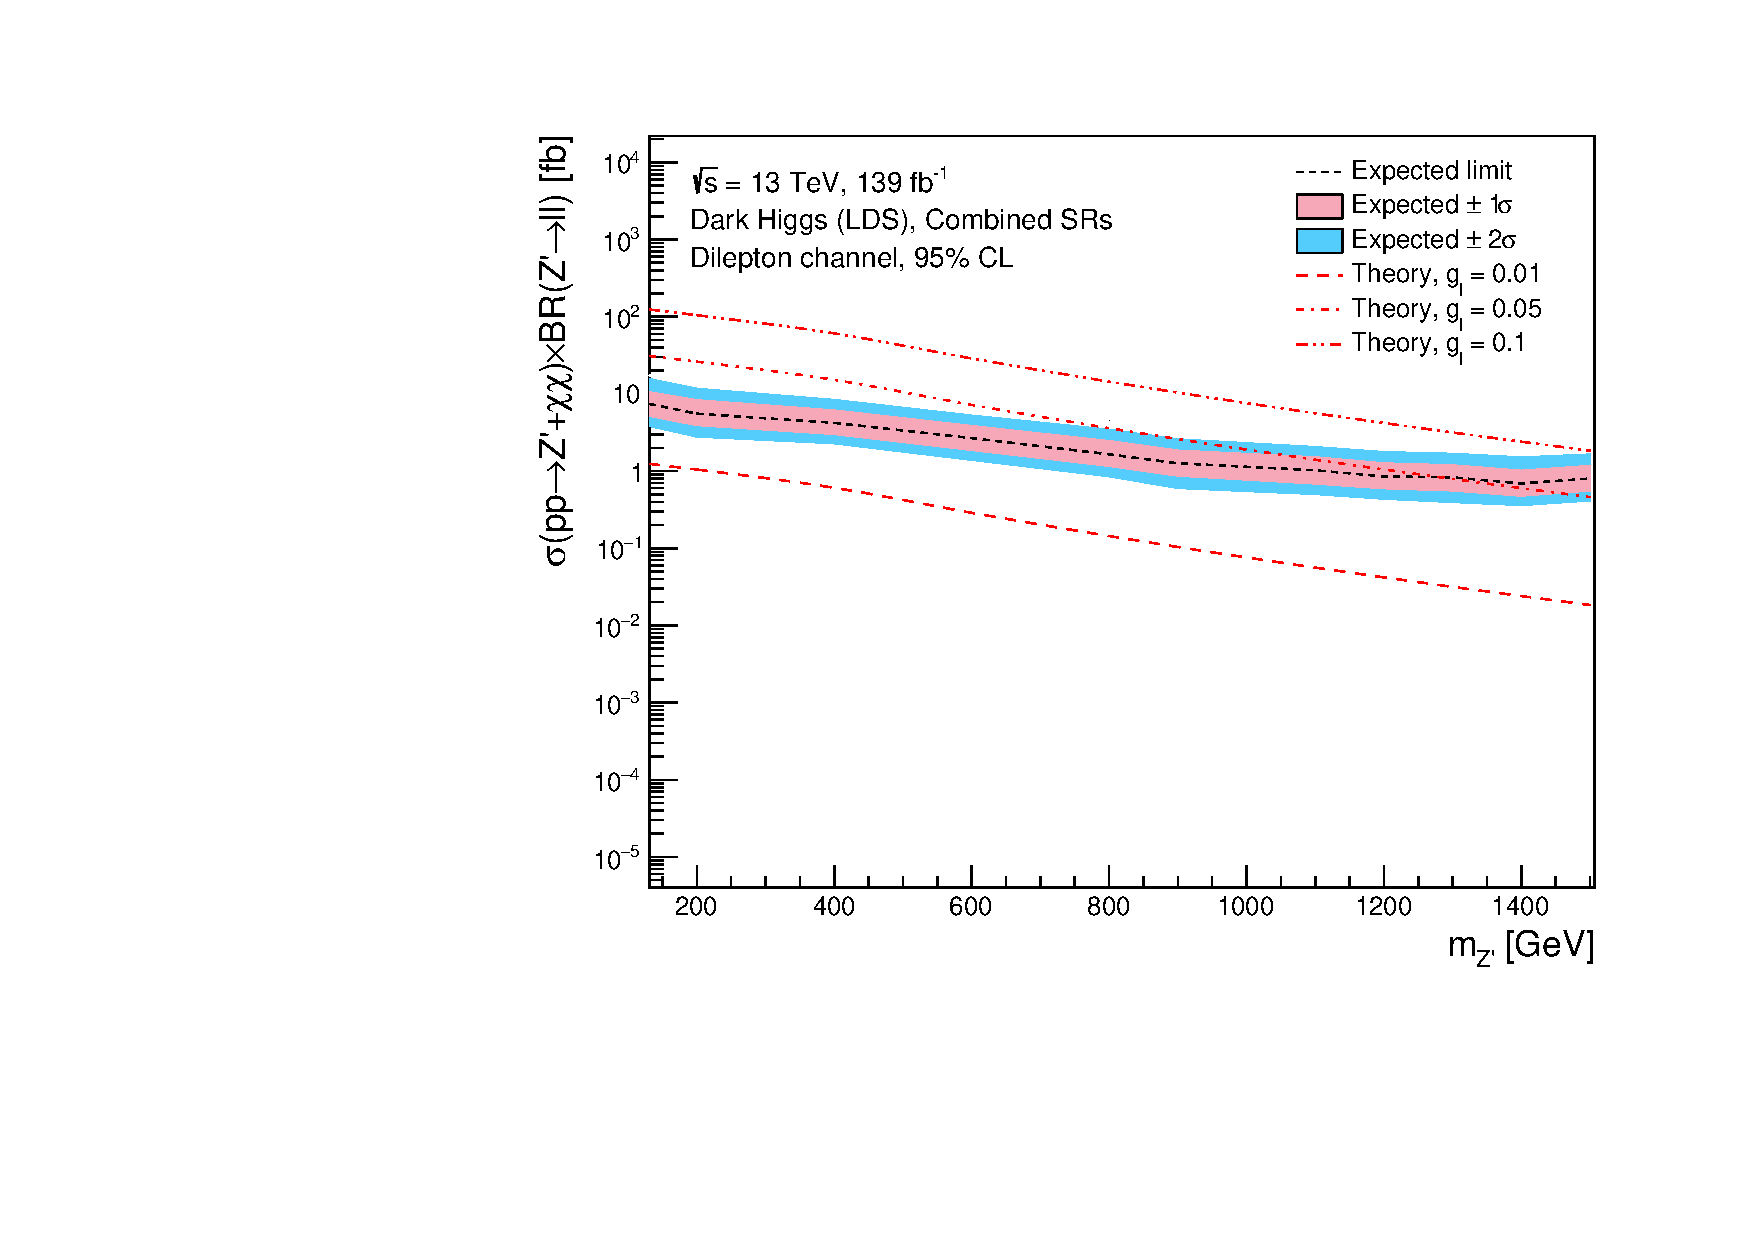
\includegraphics[width=1\textwidth]{Limits/Model_independent/DH_LDS/mass_exclusion_comb.pdf}
   \end{subfigure}
   \hfill
   \begin{subfigure}[b]{0.49\textwidth}
      \centering
      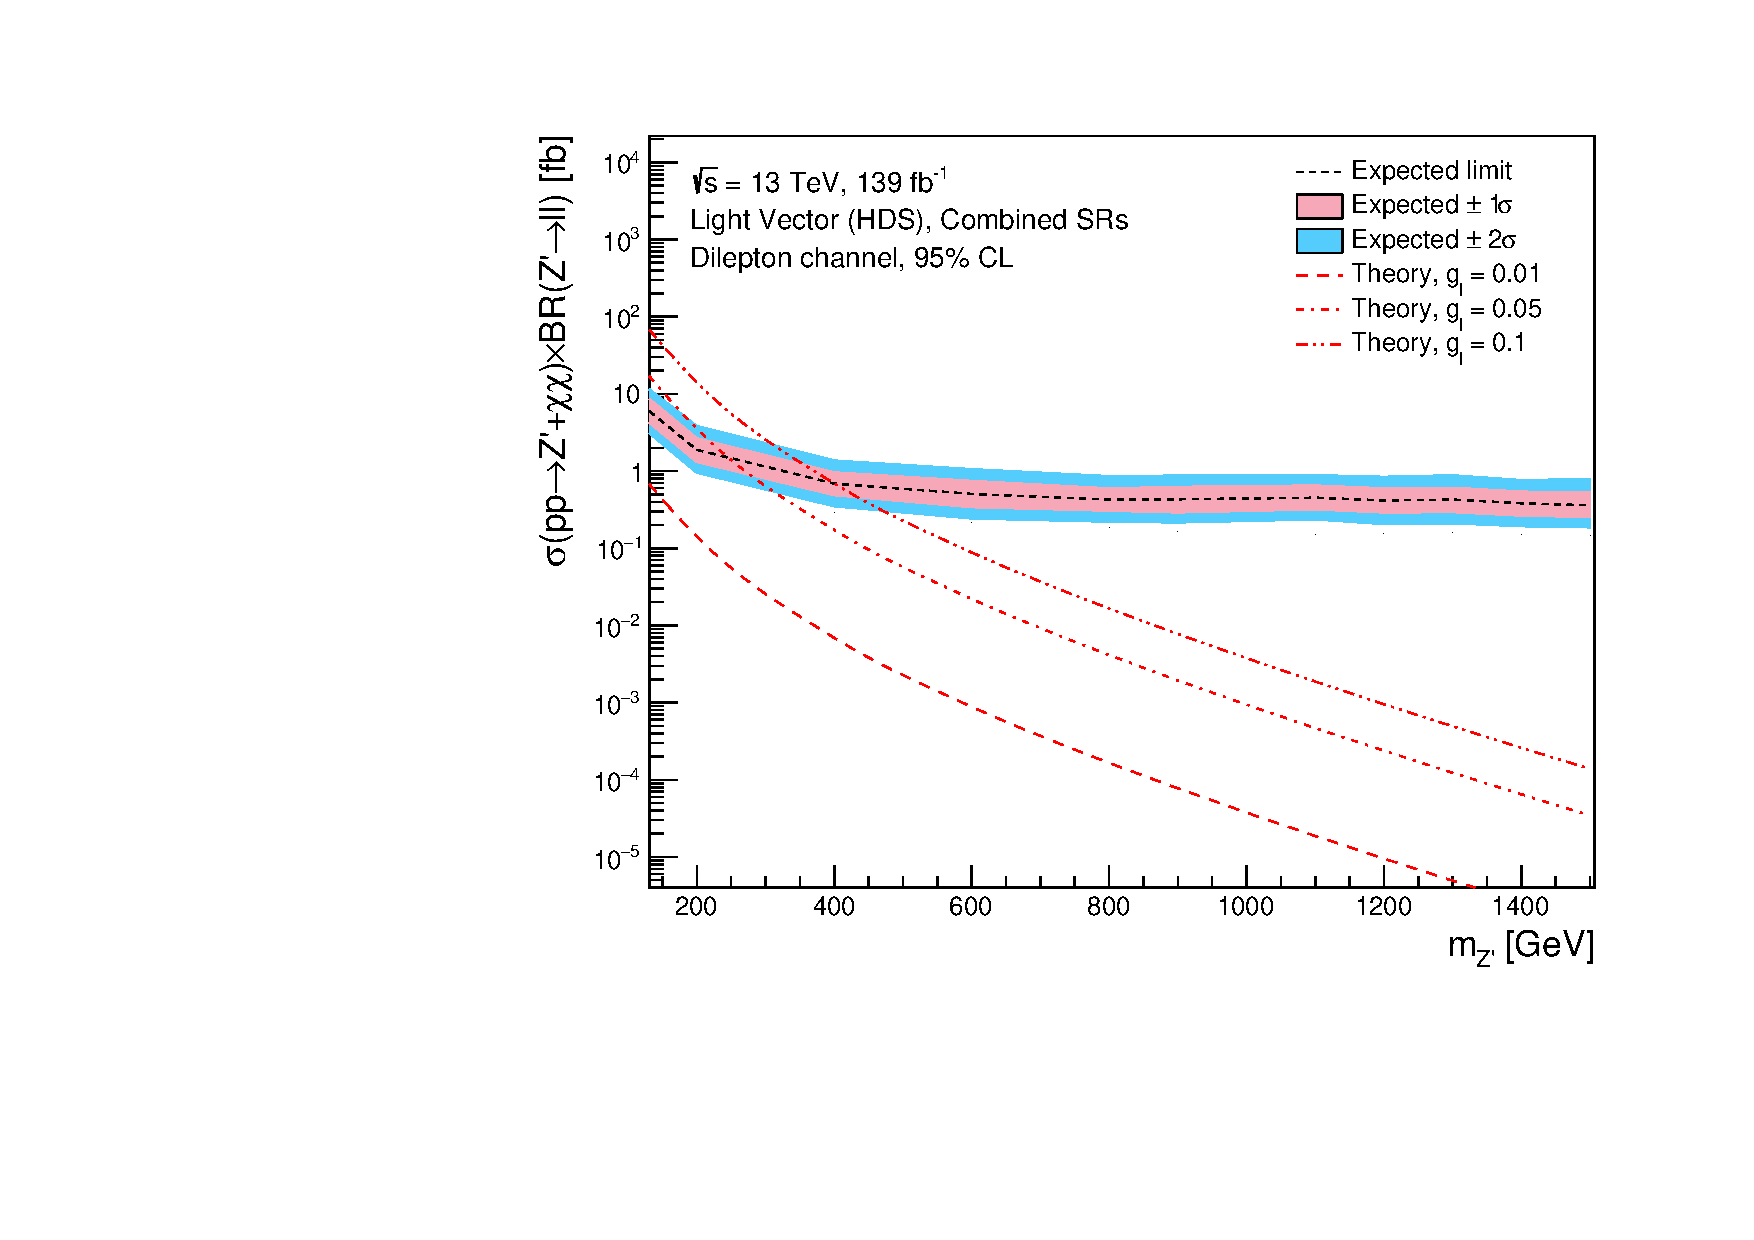
\includegraphics[width=1\textwidth]{Limits/Model_independent/LV_HDS/mass_exclusion_comb.pdf}
   \end{subfigure}
   \hfill
   \begin{subfigure}[b]{0.49\textwidth}
      \centering
      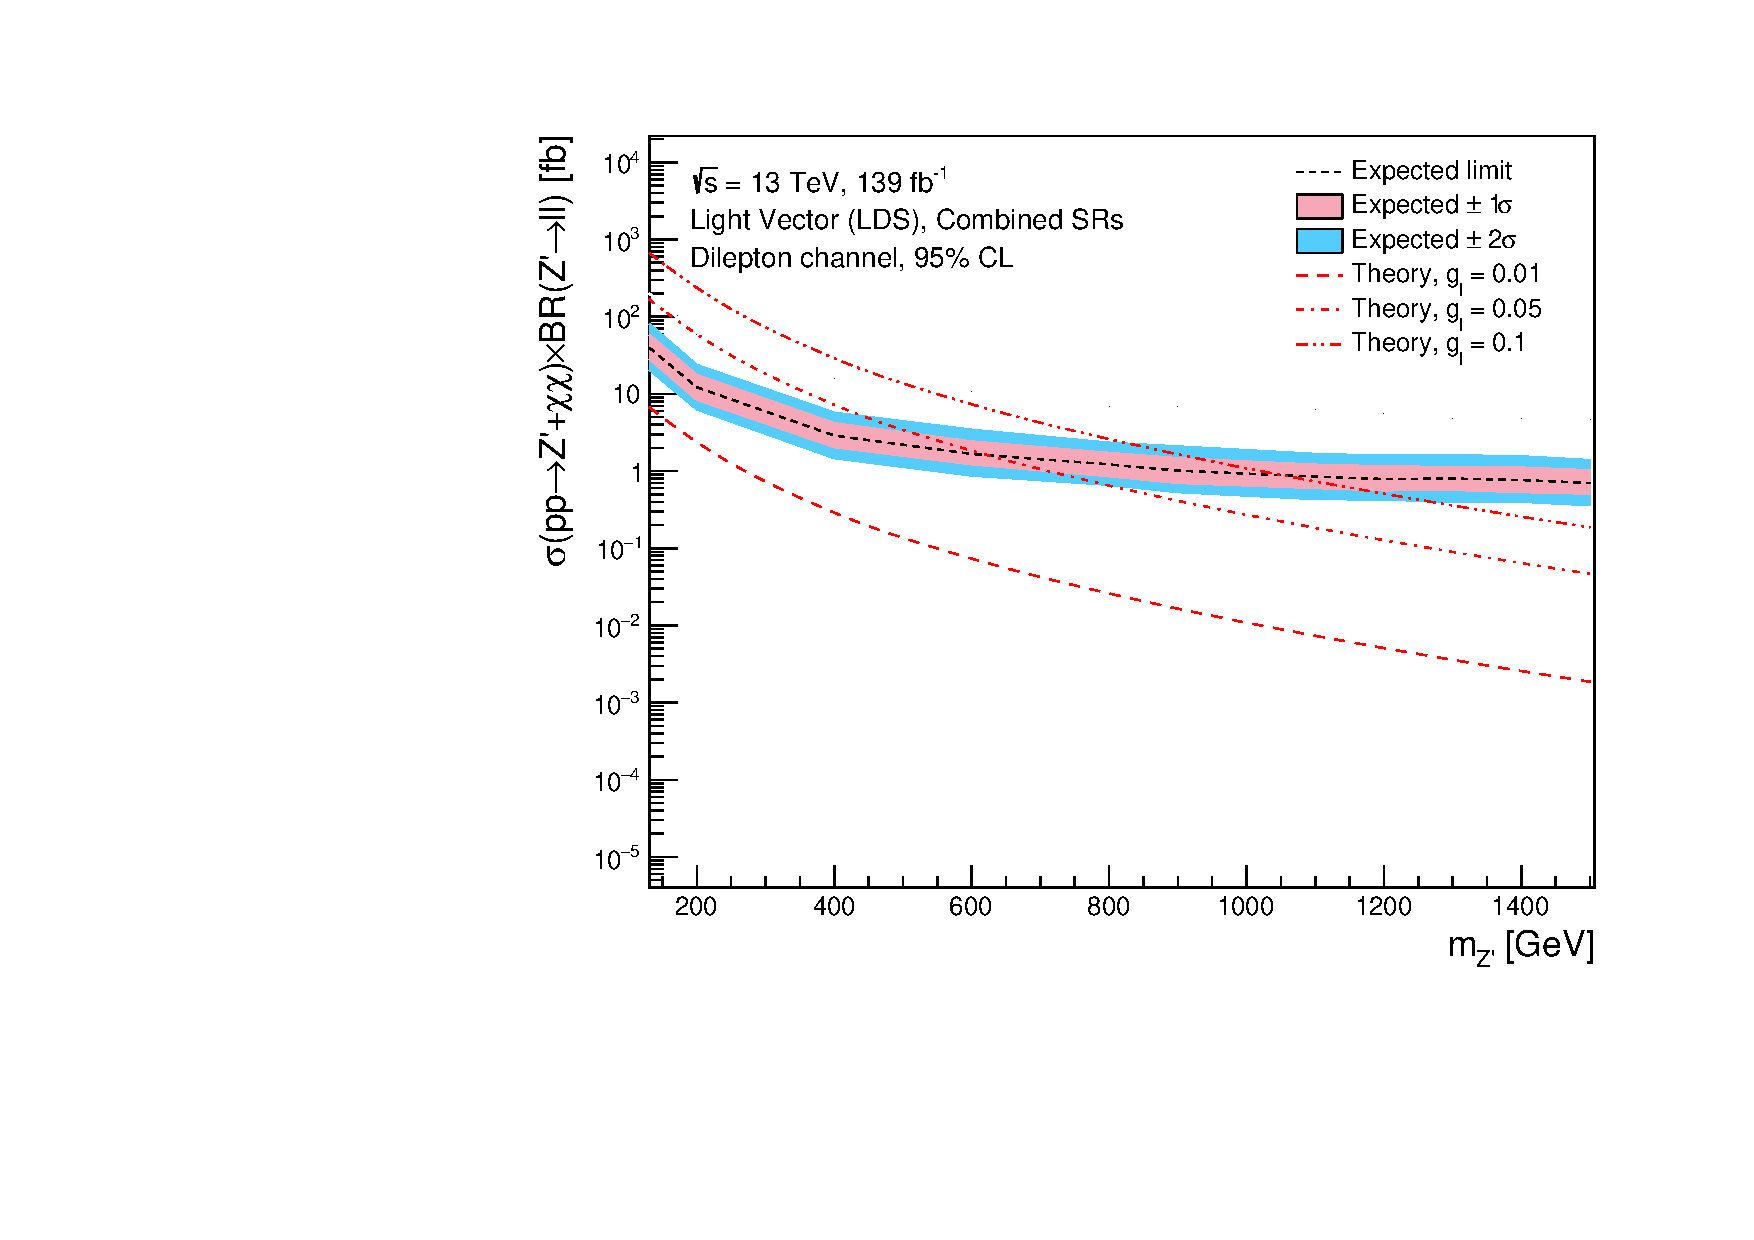
\includegraphics[width=1\textwidth]{Limits/Model_independent/LV_LDS/mass_exclusion_comb.pdf}
   \end{subfigure}
   \hfill
	\begin{subfigure}[b]{0.49\textwidth}
      \centering
      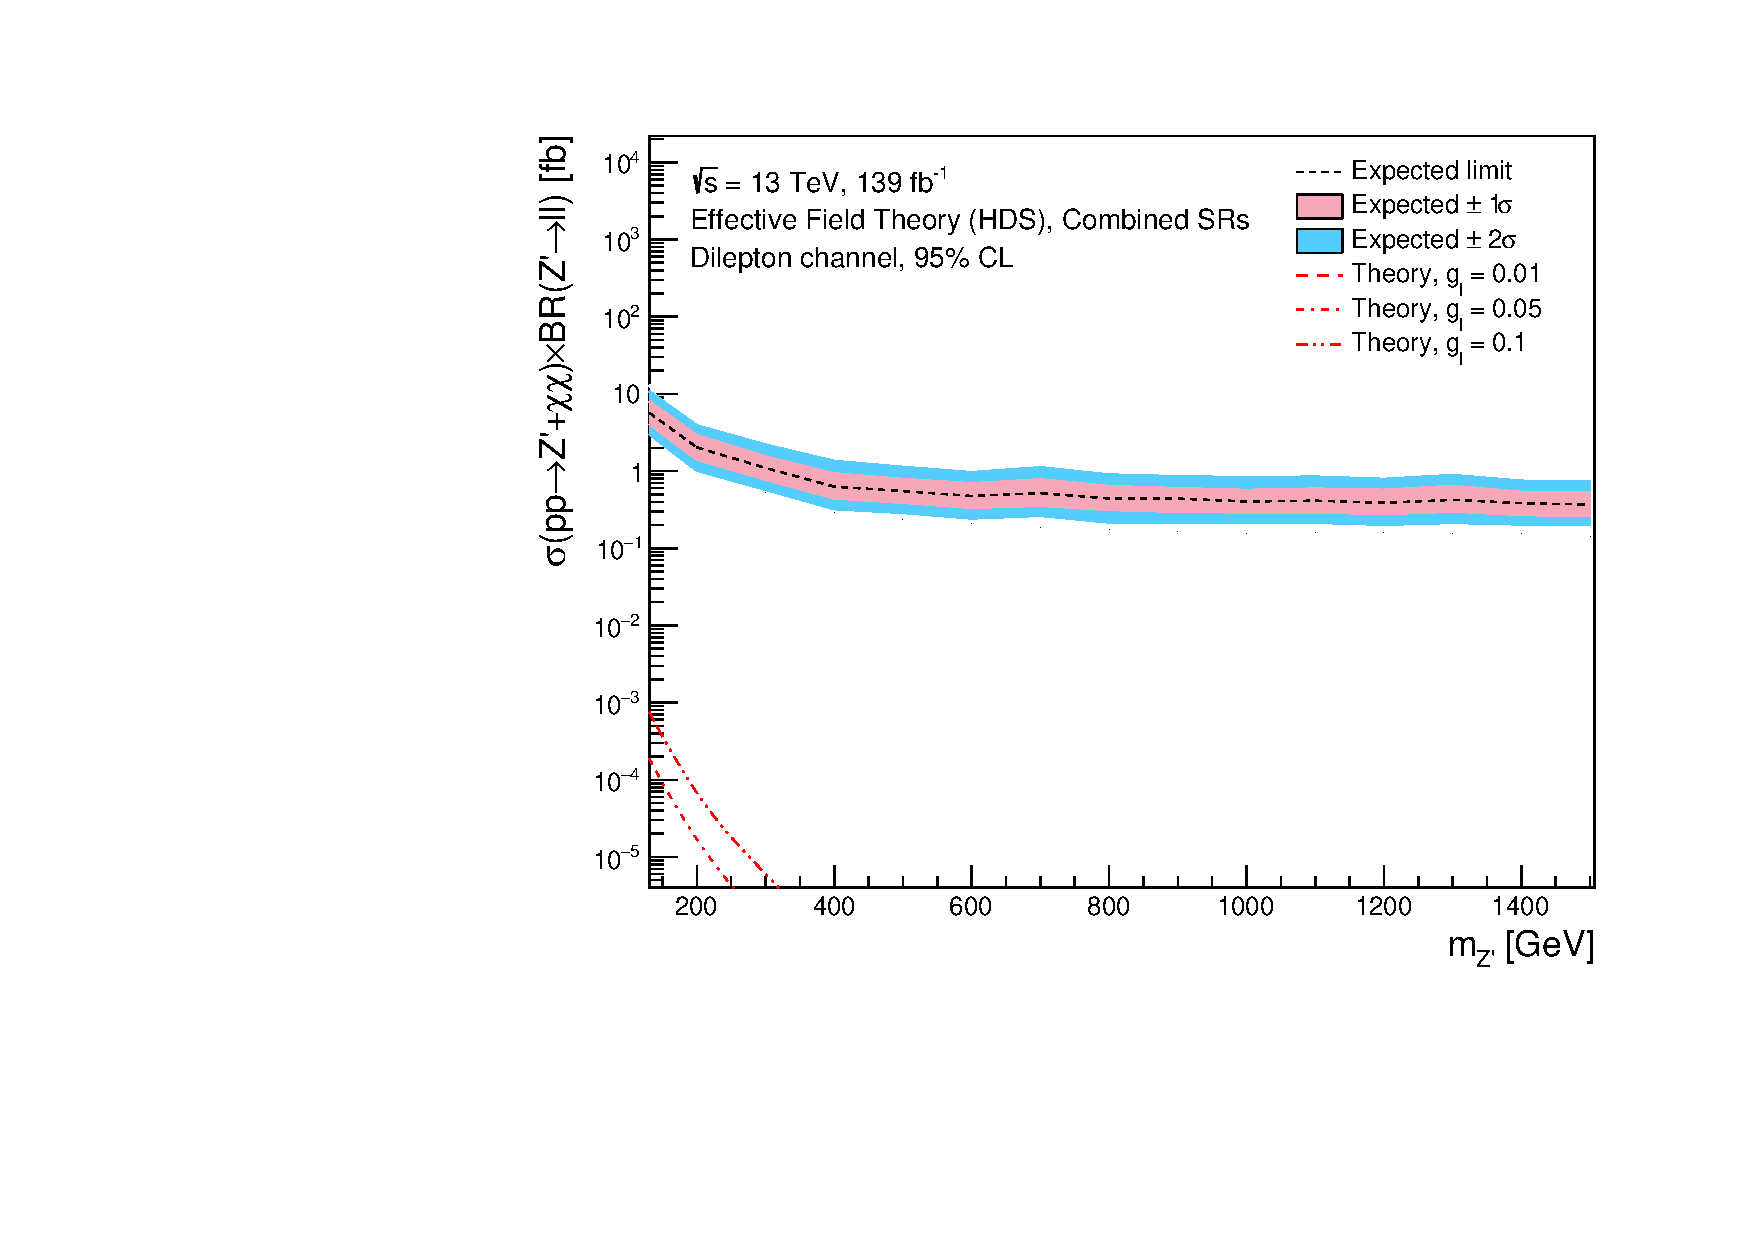
\includegraphics[width=1\textwidth]{Limits/Model_independent/EFT_HDS/mass_exclusion_comb.pdf}
   \end{subfigure}
   \hfill
   \begin{subfigure}[b]{0.49\textwidth}
      \centering
      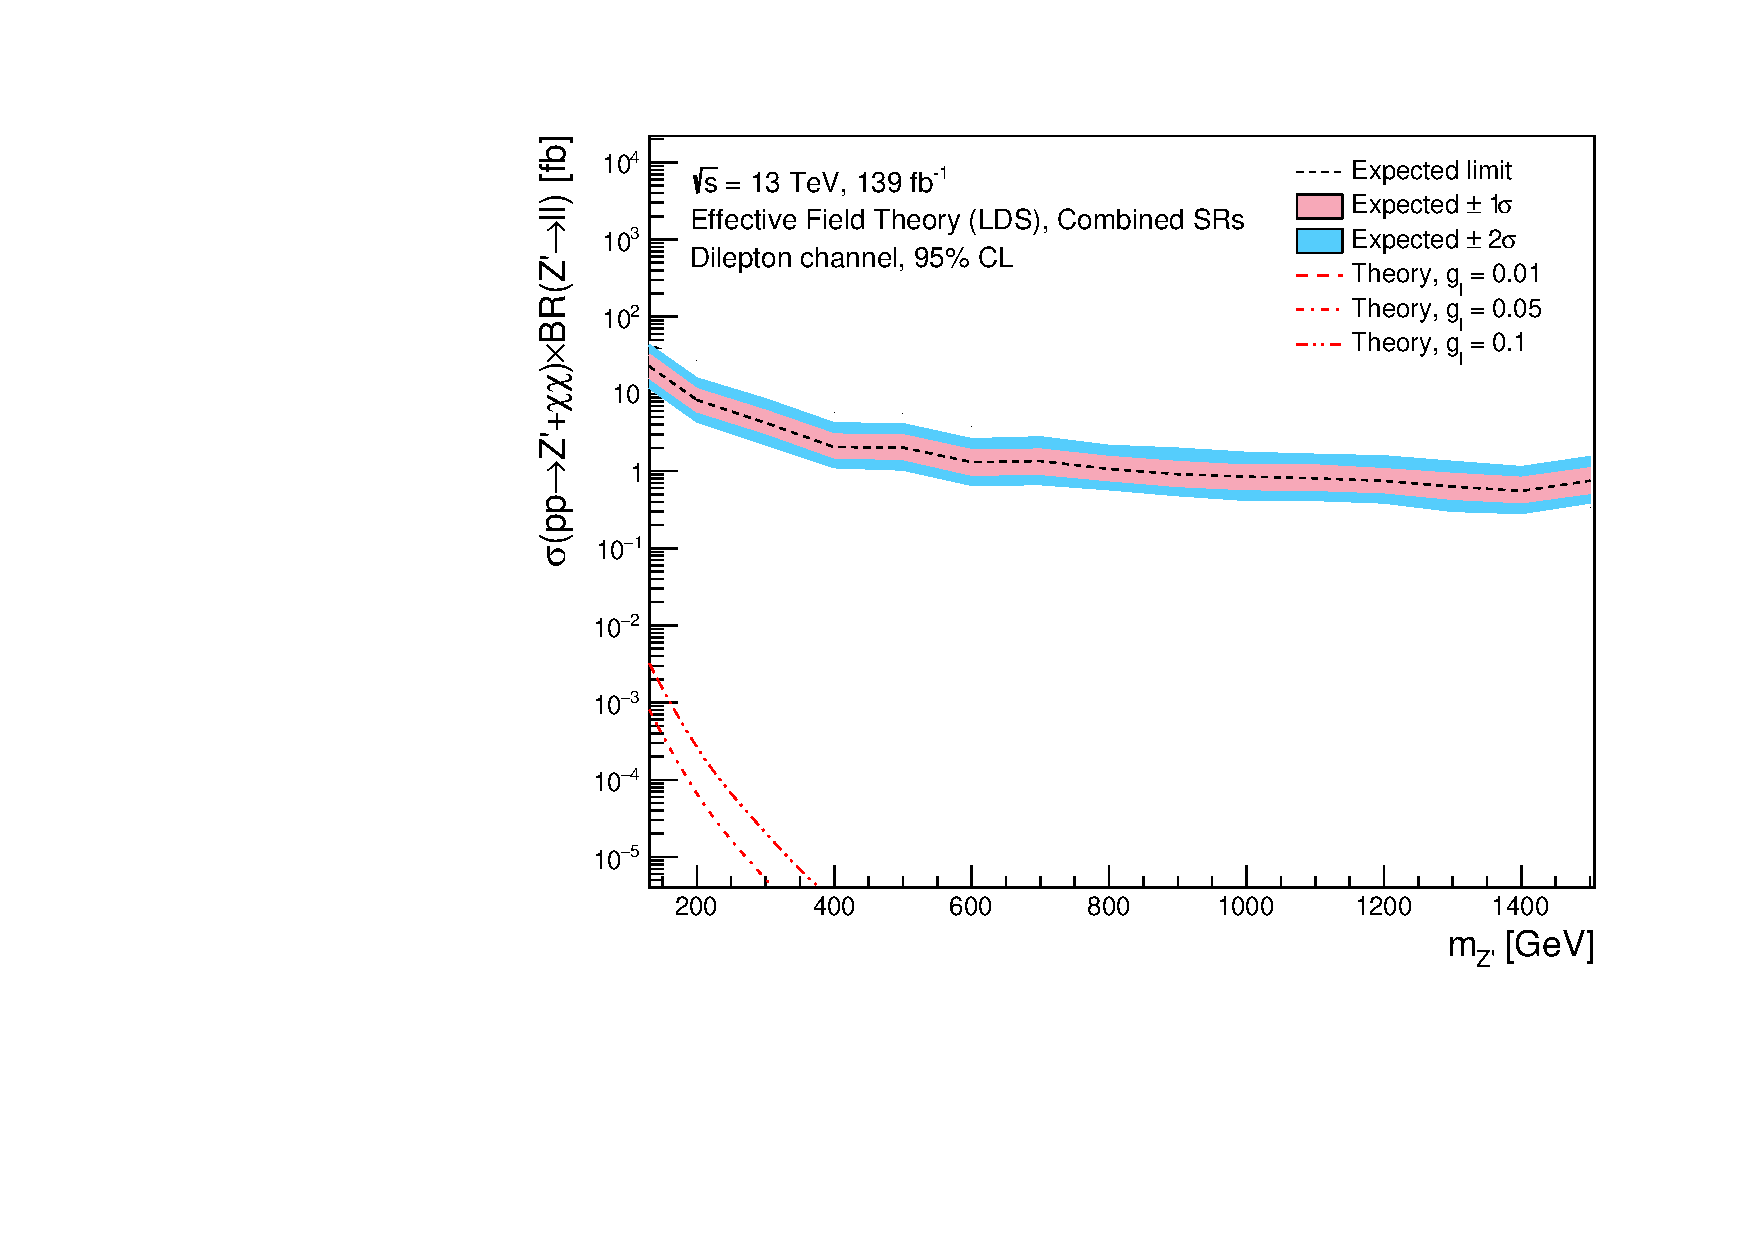
\includegraphics[width=1\textwidth]{Limits/Model_independent/EFT_LDS/mass_exclusion_comb.pdf}
   \end{subfigure}
   \caption[Mass exclusion limits of combined $ee$ and $\mu\mu$ channel for all mono-Z' models using the model independent approach]{Mass exclusion limits of combined $ee$ and $\mu\mu$ channel for all mono-Z' models in both the Heavy Dark Sector (HDS) and Light Dark Sector (LDS) using the model independent approach. 
   In the top row we have the mass exclusion of the Dark Higgs HDS (left) and Dark Higgs LDS (right) models. In the middle row we have the mass exclusions of the Light Vector HDS (left) and Light Vector LDS (right) models. In the bottom row we have the mass exclusion of the 
   inelastic EFT HDS (left) and inelastic EFT LDS (right) models.
   The y-axis on all plots represents the cross-section times branching ratio of the process we are studying. The x-axis is the mass of the $Z'$ boson. We did not interpolate between the available masses we had simulated, 
   and have rather just connected the values calculated for each mass point by connecting the points. The dashed black line is the expected 95\% CL limit calculated using Bayesian statistics with a 1$\sigma$ and 2$\sigma$ deviation. 
   The different dashed lines represent the theoretical cross-section times branching ratio of the process when varying the value of the lepton coupling $g_l$ between the leptons and the $Z'$ boson. The simulated events in this thesis utilized the value $g_l=$ 0.01, we include the cross-section times branching ratio when increasing this coupling to 0.05 and 0.1 to see how the exclusions change. 
   }\label{fig:model_indep_mono_Zp_excl}
\end{figure}


\clearpage
\section{Comparison of results}\label{sec:comparisons_of_methods}
To more easily compare the model dependent approach, where we train one network for every DM model using all the available simulated events, to the model independent approach, where we train three networks in kinematically orthogonal regions containing every simulated event for all DM models, 
we present a side by side comparison of the expected mass exclusion plots. To remind how these plots work, the goal is to exclude as many of the mass points as possible. For the one-dimensional mono-$Z'$ exclusions, we want as much of the theoretical cross-section times branching ratio to be over the expected 95\% CL limit. 
While for the two-dimensional exclusions (SUSY and 2HDM + a), we want as many of the mass points to be inside the 95\% CL limit as these are excluded.\\
\\In Figure \ref{fig:comp_nonZp} we can see the comparison of the direct slepton production model (upper row) and the Two Higgs Doublet Model with an additional pseudoscalar $a$ model (lower row). 
The comparisons of the mono-$Z'$ models, the Dark Higgs, Light Vector and inelastic EFT can be seen in Figure \ref{fig:comp_HDS} for the Heavy Dark Sector, and Figure \ref{fig:comp_LDS} for the Light Dark Sector. For every single model we see that the model independent approach yields better results as it excludes more mass points.
\begin{figure}[!ht]
	\centering
	\begin{subfigure}[b]{0.49\textwidth}
      \centering
      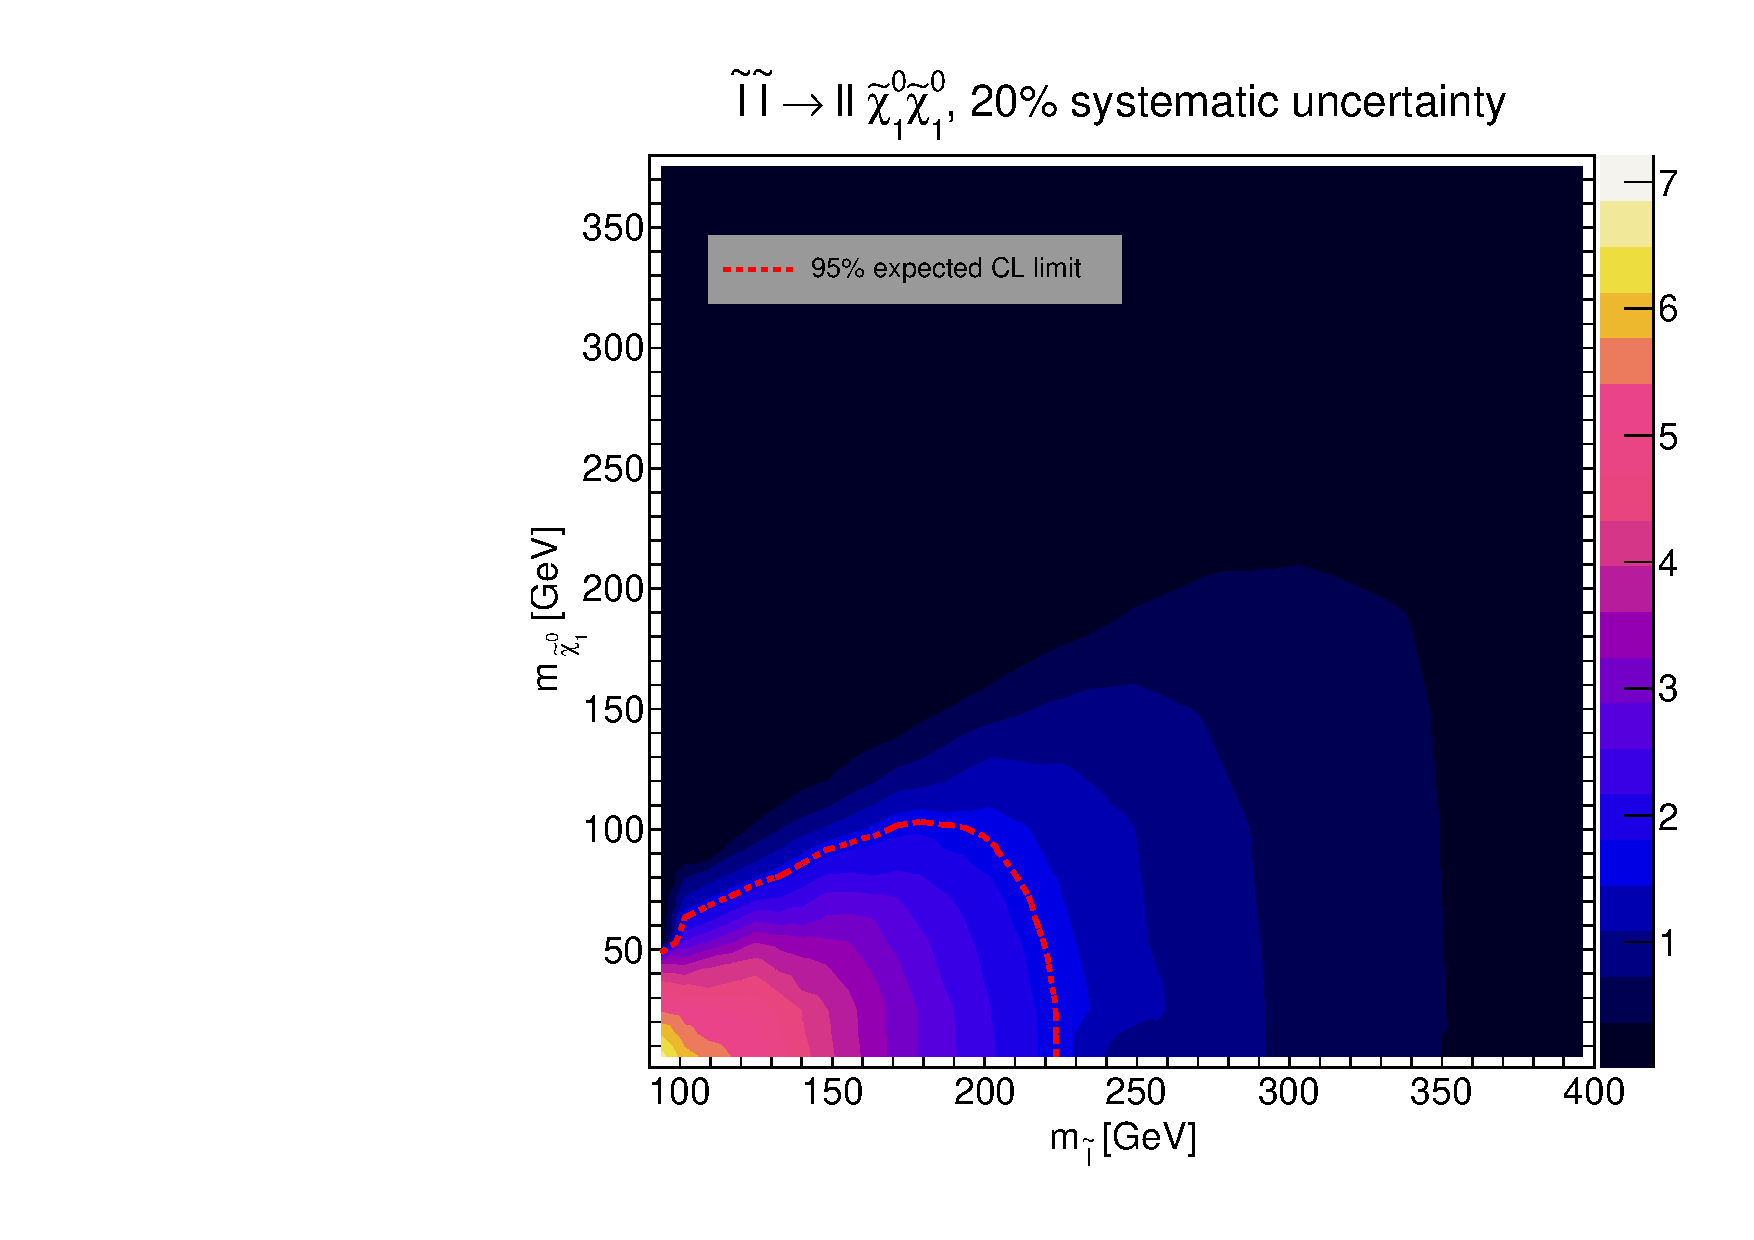
\includegraphics[width=1\textwidth]{Limits/SlepSlep/SlepSlep_ll.pdf}
   \end{subfigure}
   \hfill
	\begin{subfigure}[b]{0.49\textwidth}
      \centering
      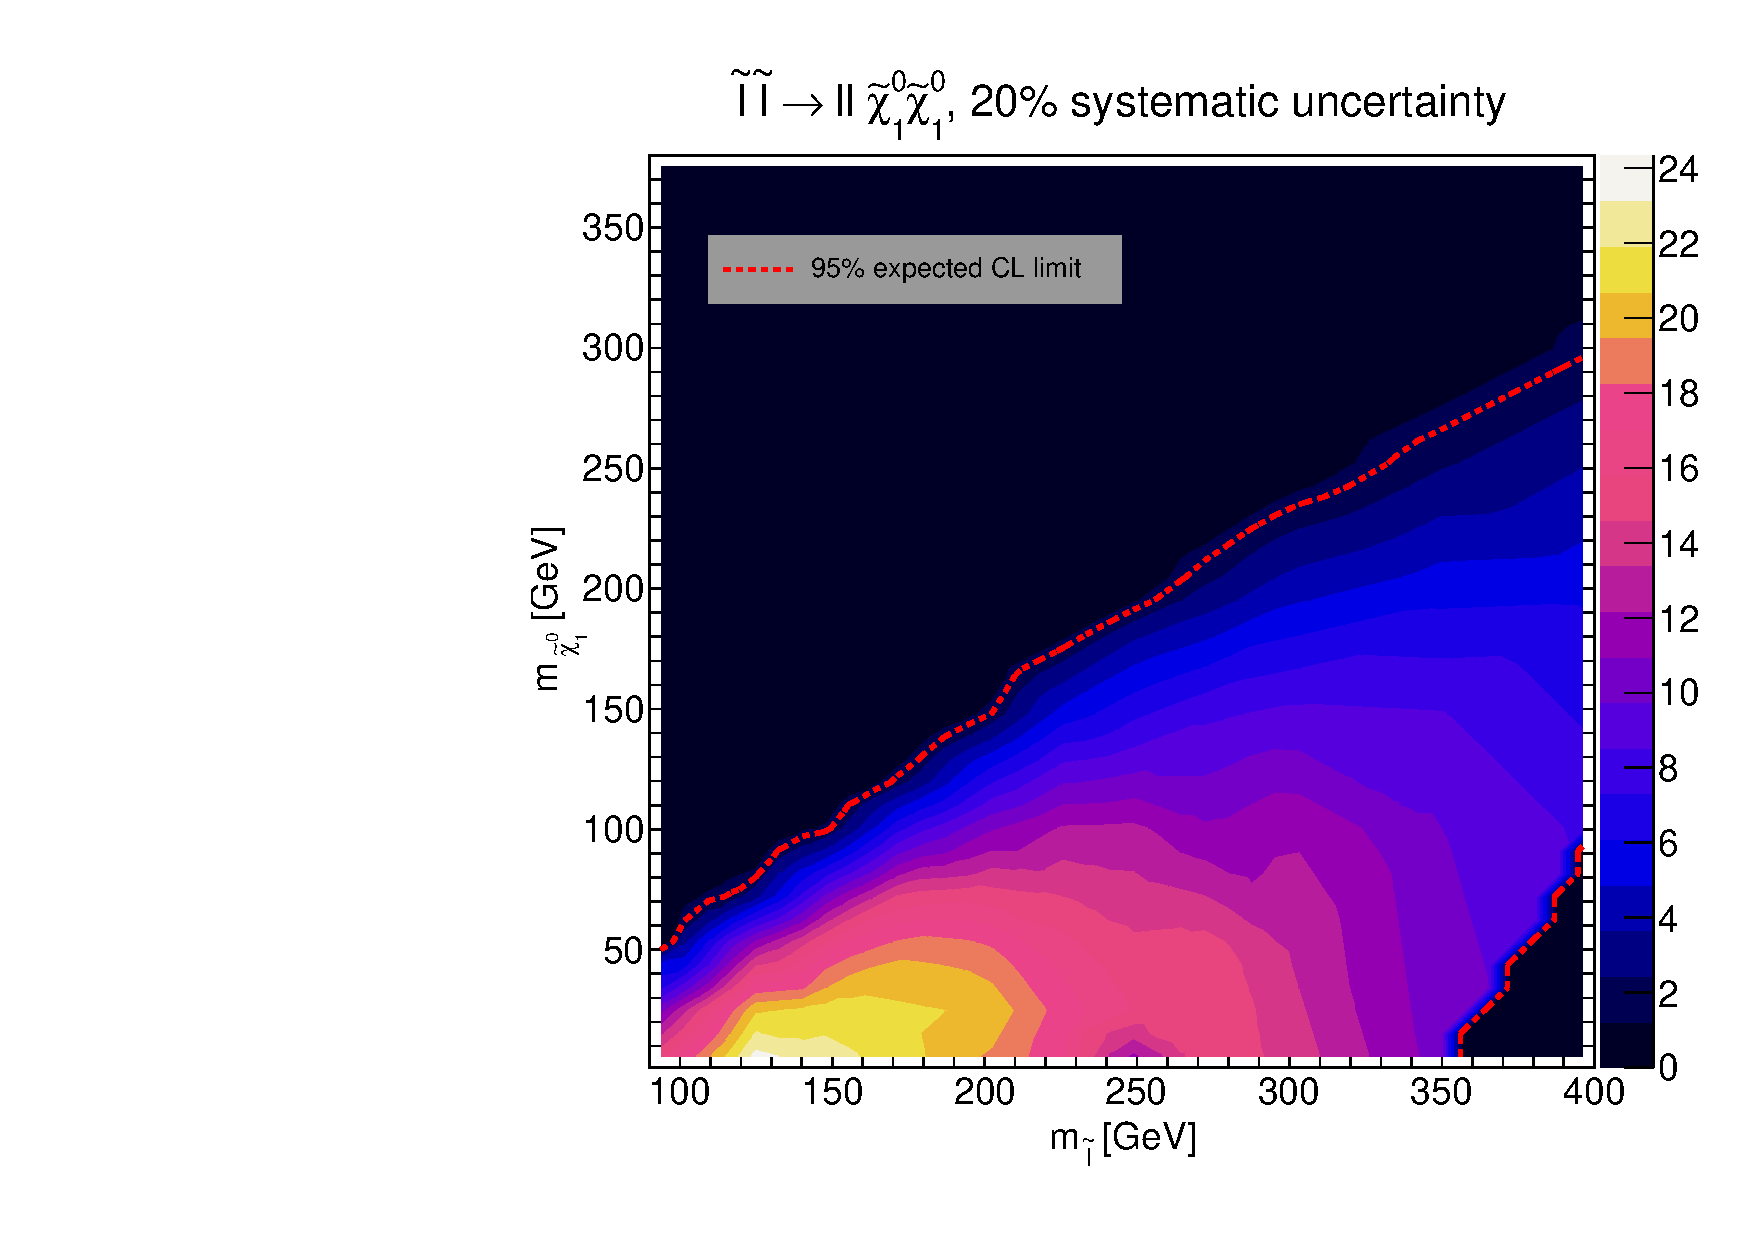
\includegraphics[width=1\textwidth]{Limits/Model_independent/SlepSlep/SlepSlep_ll.pdf}
   \end{subfigure}
   \hfill
   \begin{subfigure}[b]{0.49\textwidth}
      \centering
      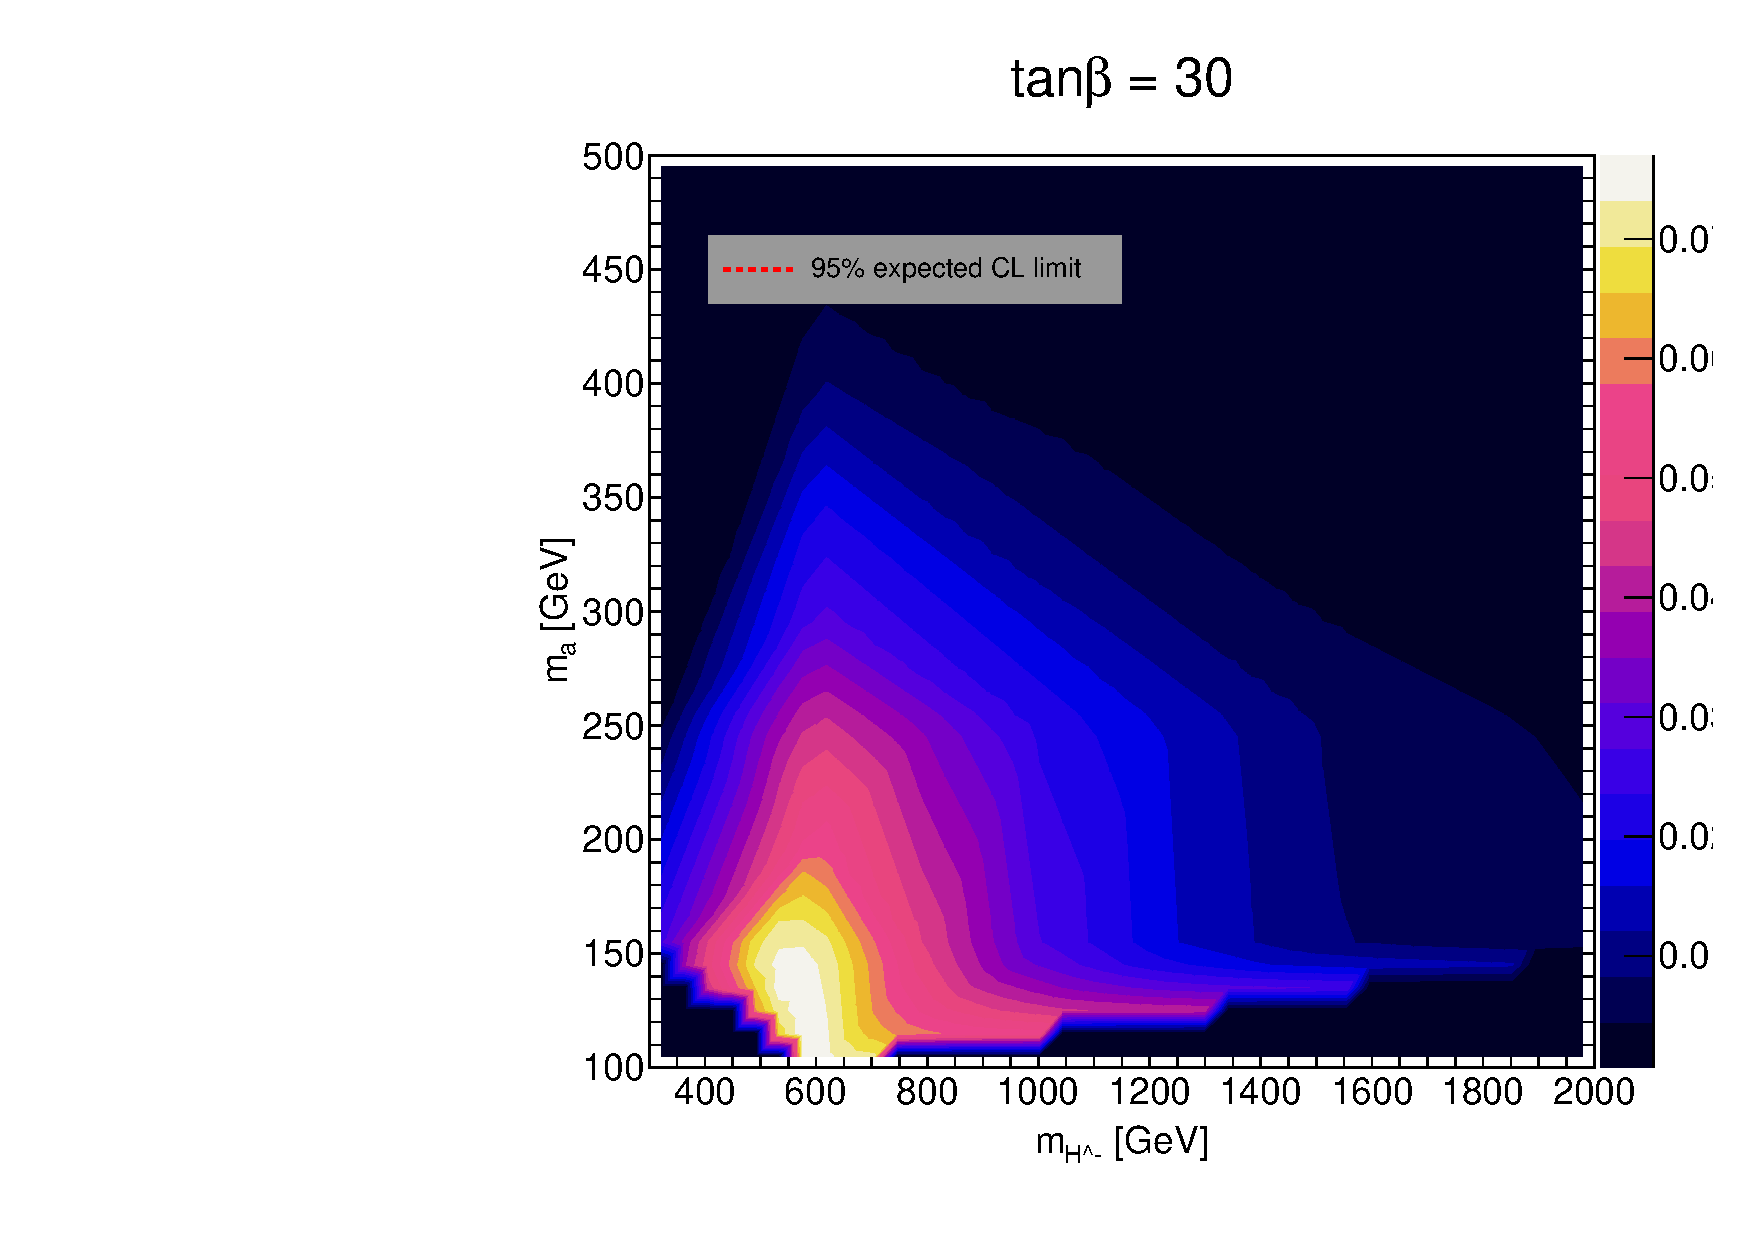
\includegraphics[width=1\textwidth]{Limits/2HDM/2HDM_ll_tb30.pdf}
   \end{subfigure}
   \hfill
   \begin{subfigure}[b]{0.49\textwidth}
      \centering
      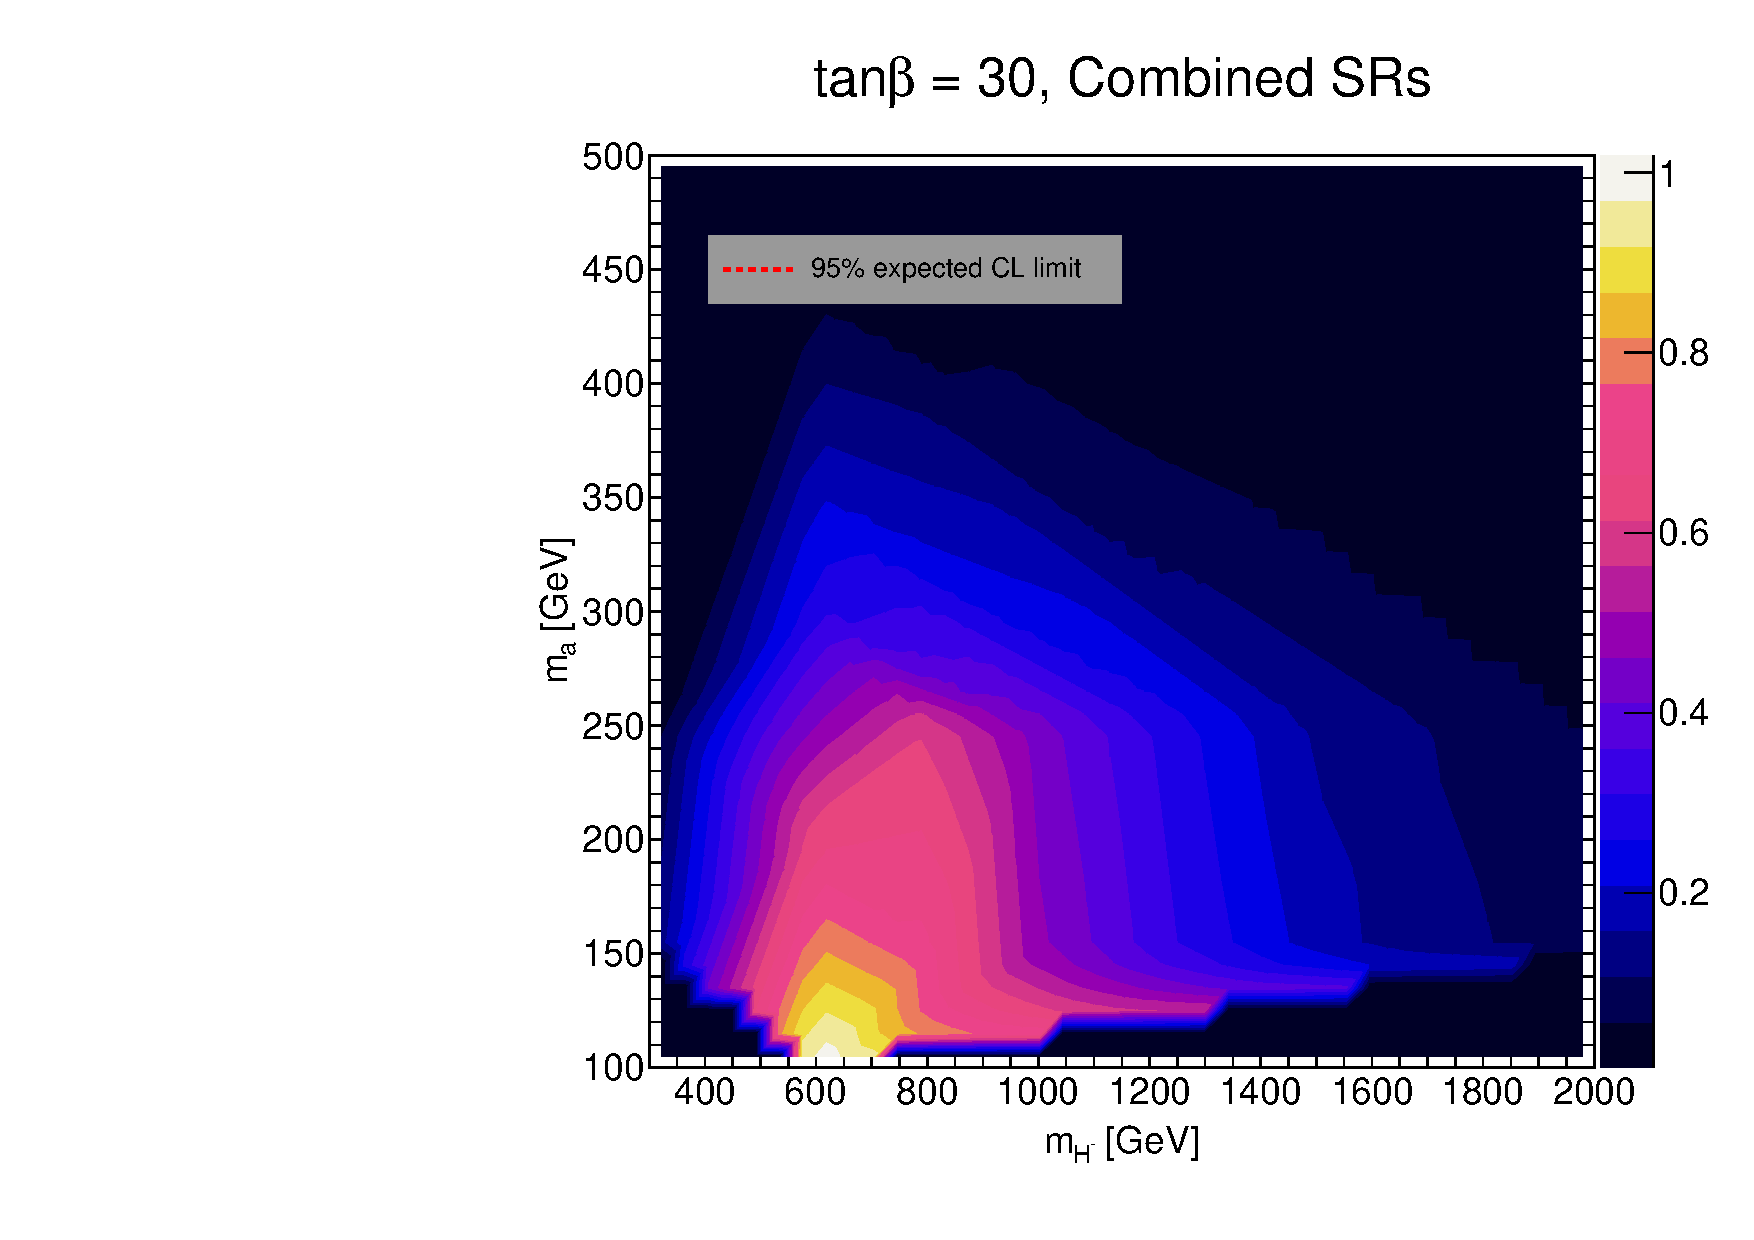
\includegraphics[width=1\textwidth]{Limits/Model_independent/2HDM/2HDM_ll_tb30.pdf}
   \end{subfigure}
   \caption[Comparison of mass exclusion limit using the model dependent and model independent approach for direct slepton production and 2HDM + a]{
      Comparison of mass exclusion limit using the model dependent (left) and model independent (right) approach for direct slepton production (upper plots) and 2HDM + a (lower plots). The plots here have the two varying masses as the axes, the z-axis is the expected significance calculated using Eq. (\ref{eq:significance}) with uncertainties. The expected 95\% CL limit was chosen using Frequentist statistics using the significance $Z=$ 1.645.   
      For the direct slepton production model we have the slepton mass, $m_{\tilde{\ell}}$, on the x-axis, and the neutralino mass on $m_{\tilde{\chi}_1^0}$ the y-axis. 
      For the 2HDM + a model we have the charged Higgs mass, $m_{H^-}$, on the x-axis, and the pseudoscalar $a$ mass $m_{a}$ on the y-axis. To see the exclusions for the other values of $\tan\beta$ on the 2HDM + a model see Appendix \ref{apx:MDA}.  
      Something to note about the direct slepton production plot (top right), is the lack of exclusions in the bottom right corner where $m_{\tilde{\ell}}>350$ GeV and $m_{\tilde{\chi}_1^0}<50$ GeV, the reason for this is because we did not have any simulated event at that mass range, 
      to see the samples we had available see Figure \ref{fig:slepslep_mass}.}\label{fig:comp_nonZp}
\end{figure}
\begin{figure}[!ht]
	\centering
	\begin{subfigure}[b]{0.49\textwidth}
      \centering
      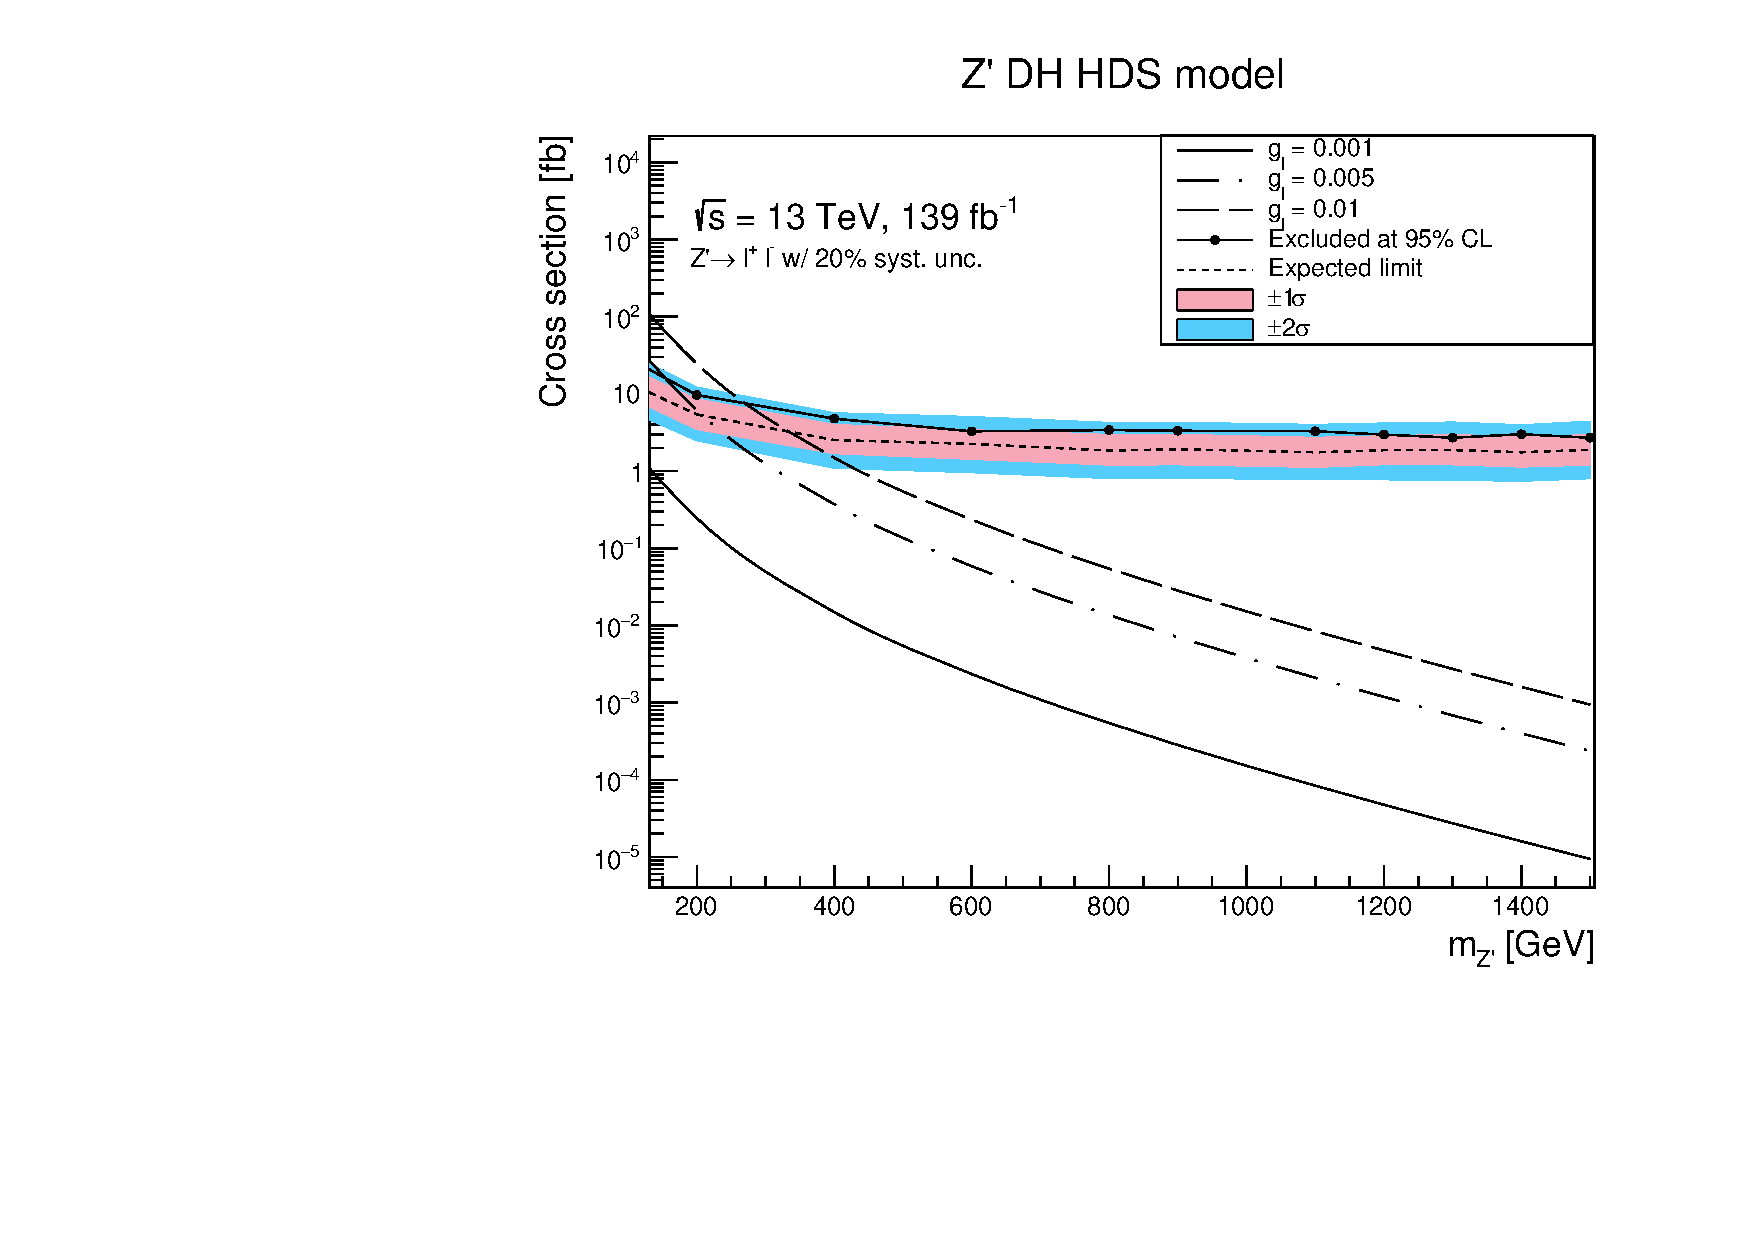
\includegraphics[width=1\textwidth]{Limits/DH_HDS/mass_exclusion_comb.pdf}
   \end{subfigure}
   \hfill
   \begin{subfigure}[b]{0.49\textwidth}
      \centering
      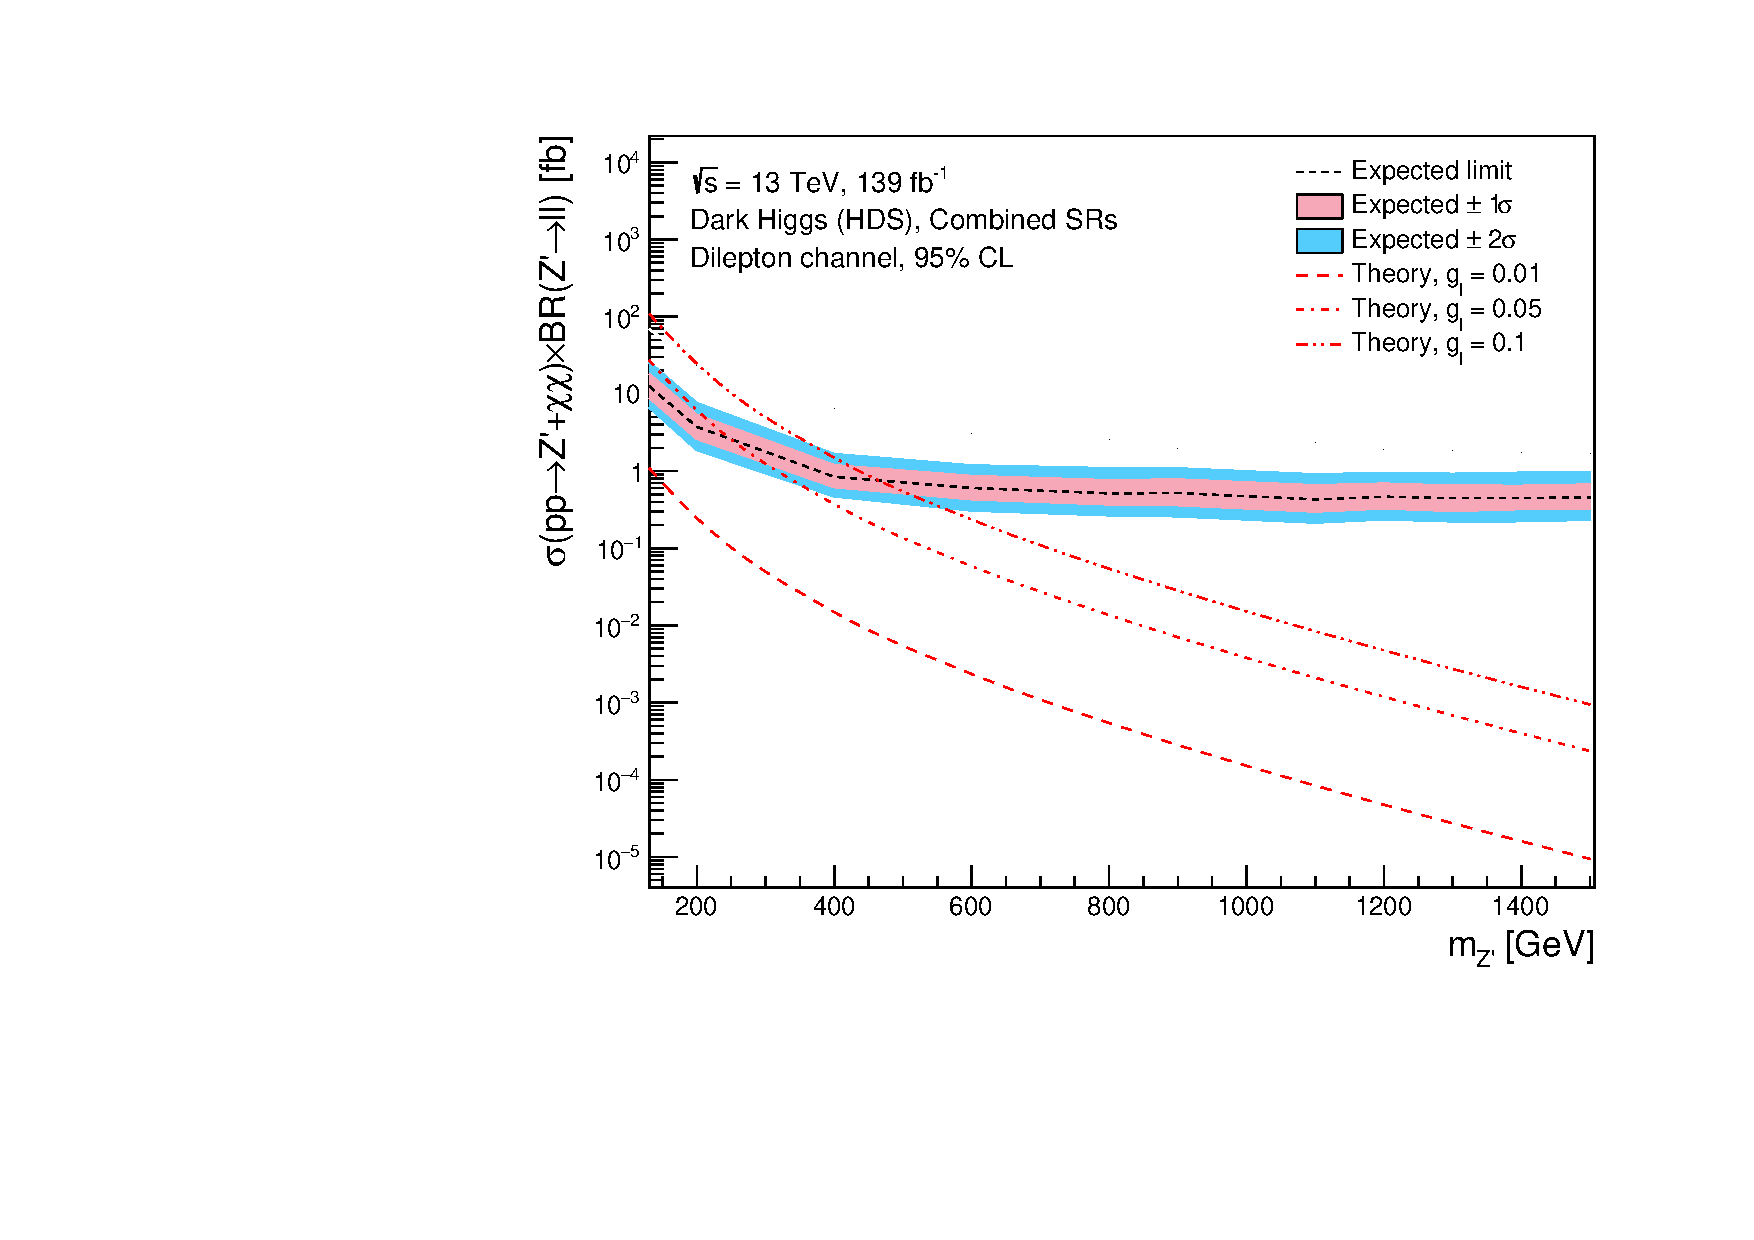
\includegraphics[width=1\textwidth]{Limits/Model_independent/DH_HDS/mass_exclusion_comb.pdf}
   \end{subfigure}
   \hfill
   \begin{subfigure}[b]{0.49\textwidth}
      \centering
      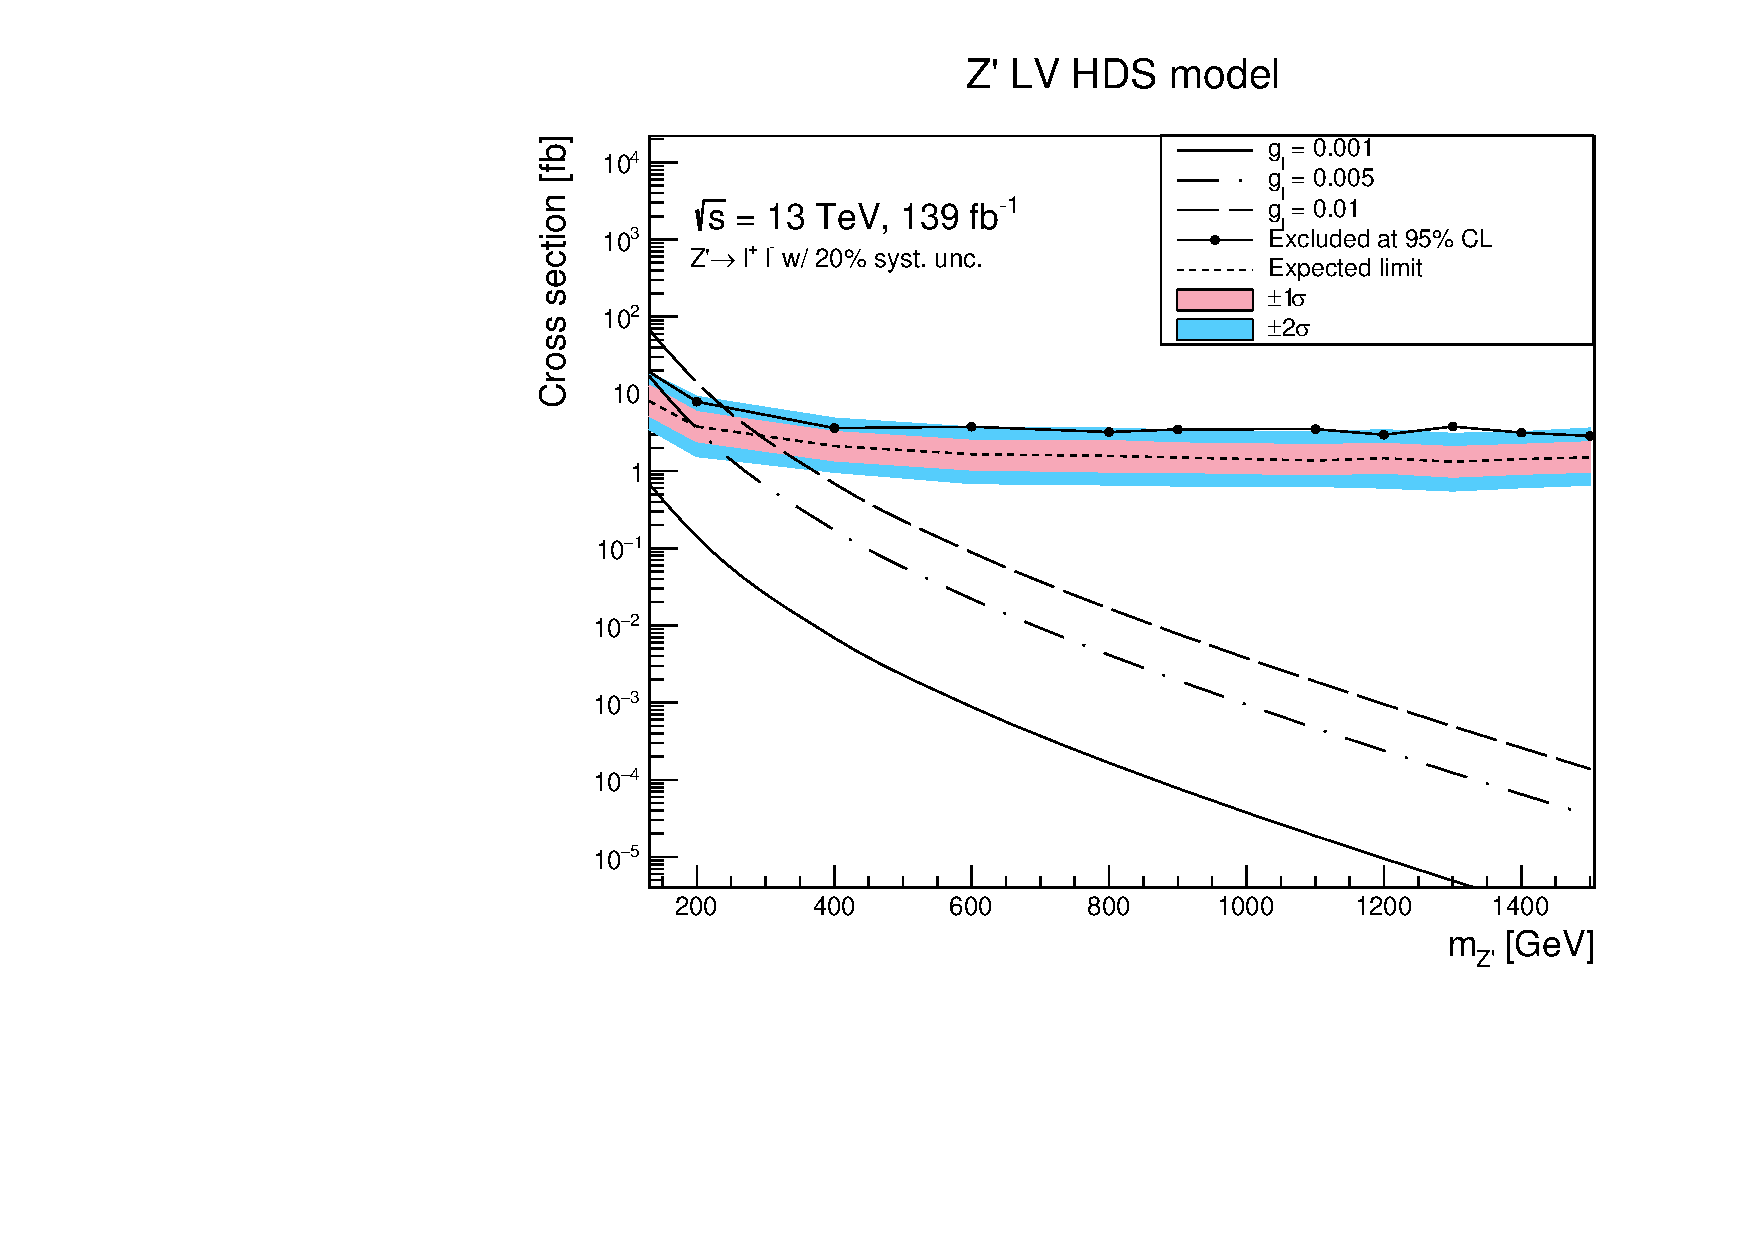
\includegraphics[width=1\textwidth]{Limits/LV_HDS/mass_exclusion_comb.pdf}
   \end{subfigure}
   \hfill
   \begin{subfigure}[b]{0.49\textwidth}
      \centering
      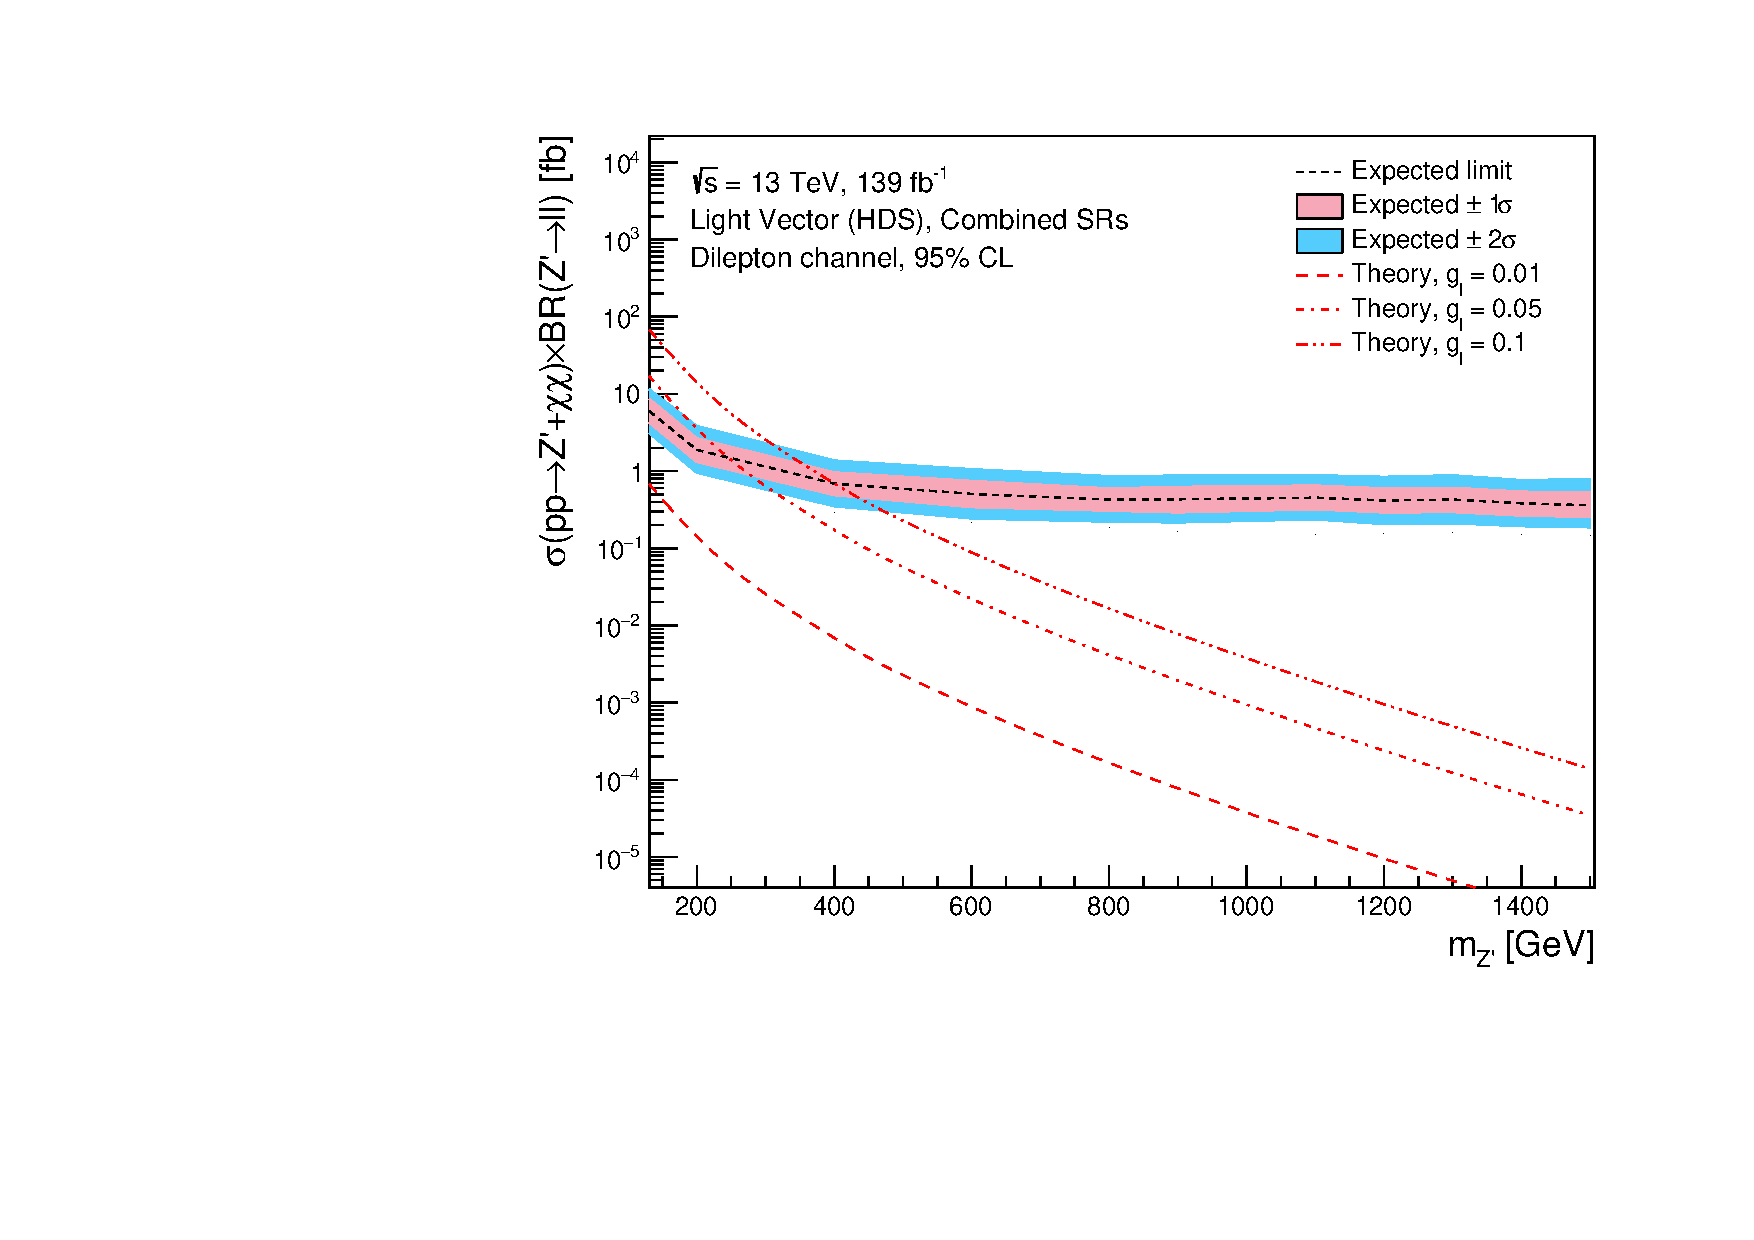
\includegraphics[width=1\textwidth]{Limits/Model_independent/LV_HDS/mass_exclusion_comb.pdf}
   \end{subfigure}
   \hfill
	\begin{subfigure}[b]{0.49\textwidth}
      \centering
      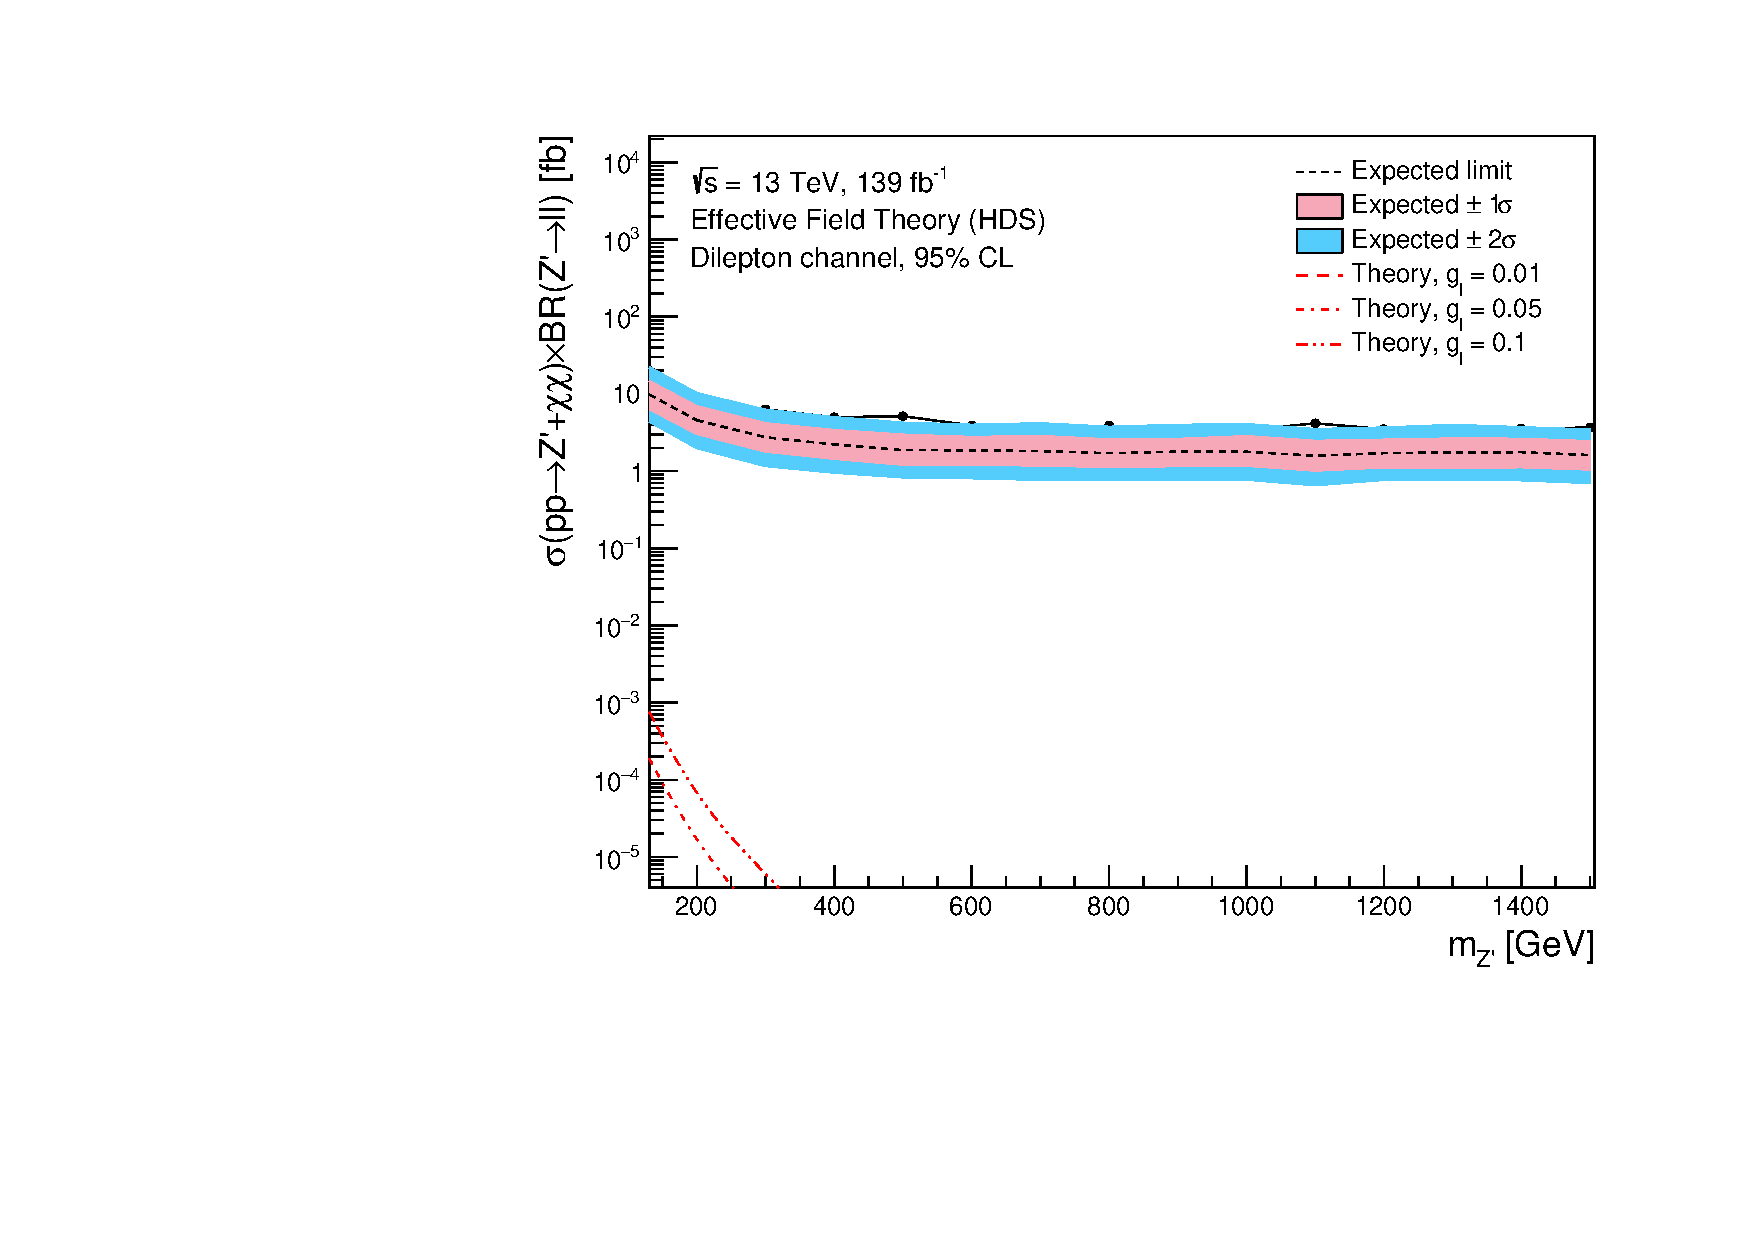
\includegraphics[width=1\textwidth]{Limits/EFT_HDS/mass_exclusion_comb.pdf}
   \end{subfigure}
   \hfill
   \begin{subfigure}[b]{0.49\textwidth}
      \centering
      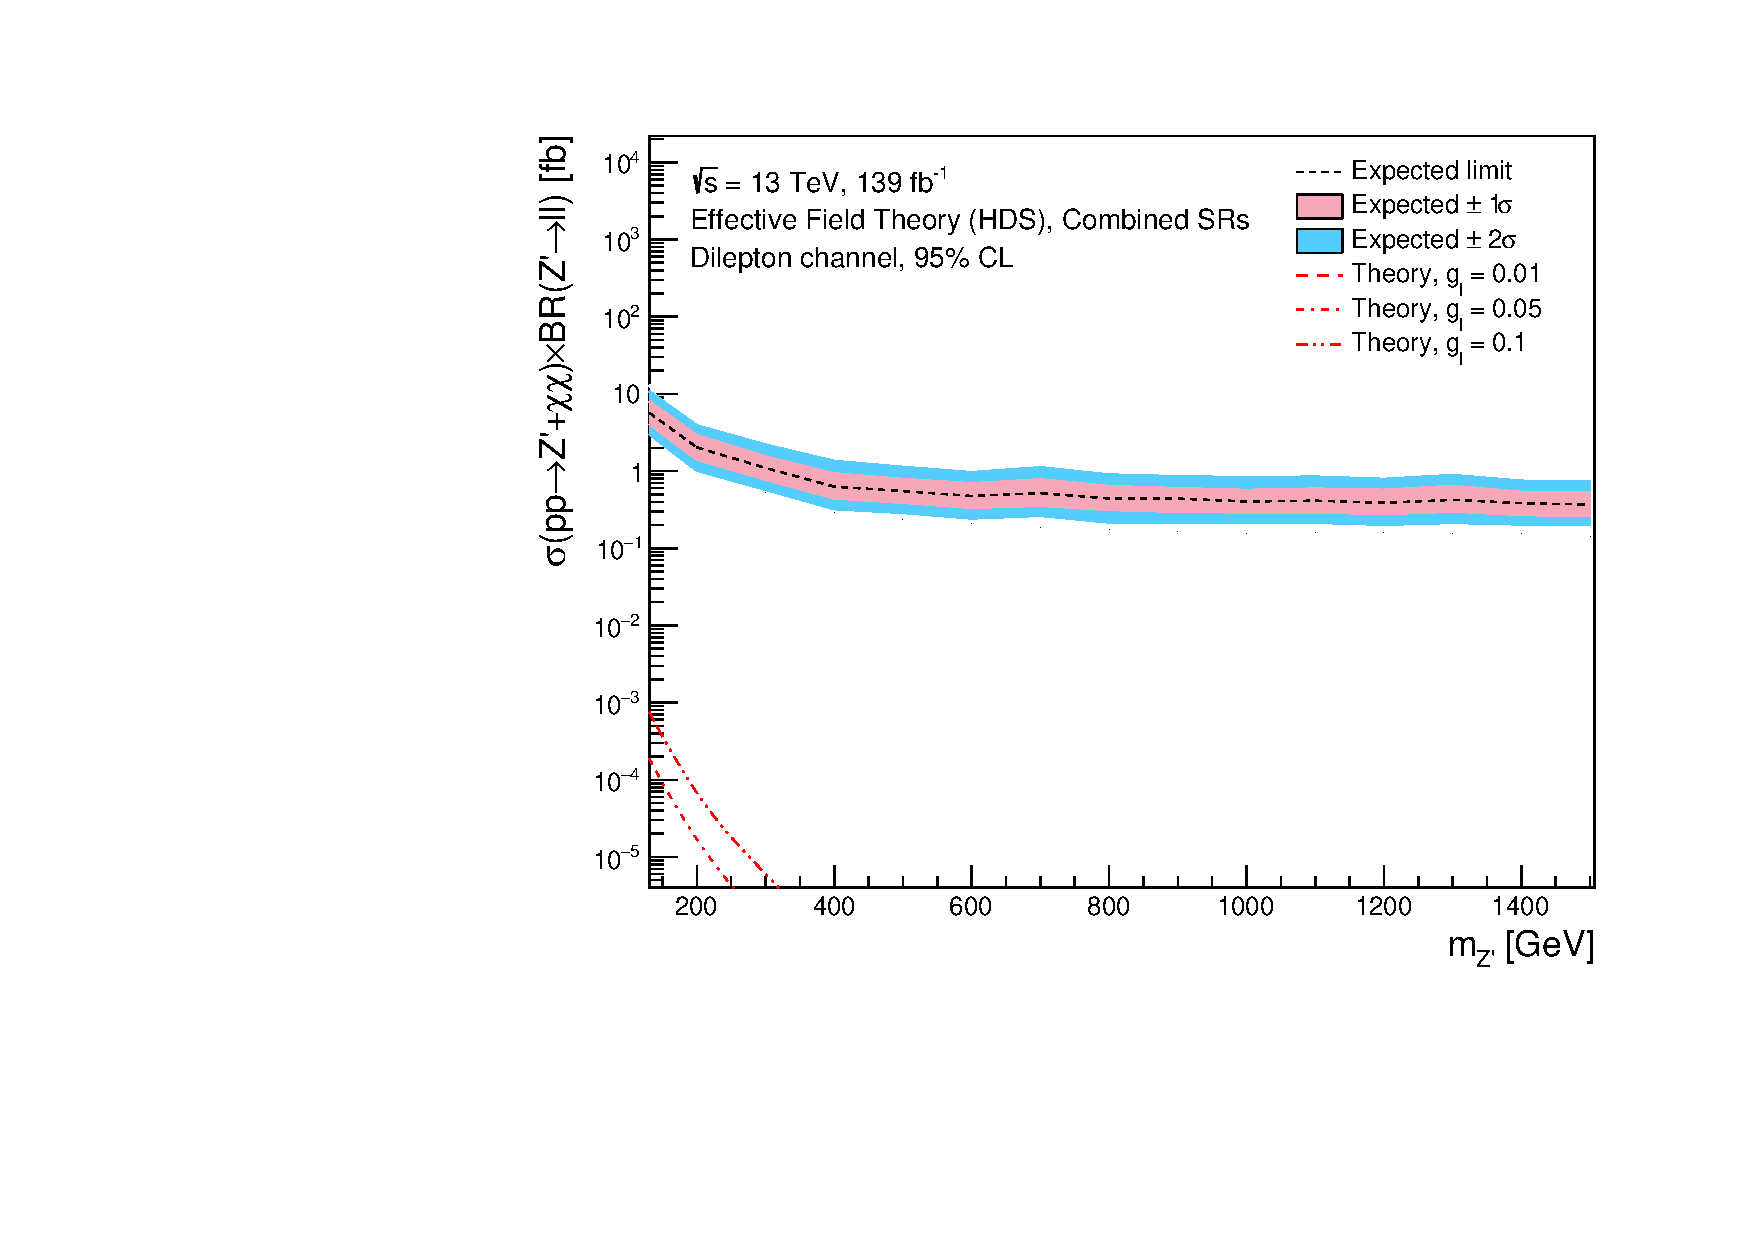
\includegraphics[width=1\textwidth]{Limits/Model_independent/EFT_HDS/mass_exclusion_comb.pdf}
   \end{subfigure}
   \caption[Comparison of mass exclusion limits of dilepton channel for all mono-Z' models using the model dependent and independent approach in the HDS]{Comparison of the mass exclusion limits of combined $ee$ and $\mu\mu$ channel for all mono-Z' models using the model dependent approach (left) and model independent approach (right) in the Heavy Dark Sector (HDS). 
   In the top row we have the mass exclusion of the Dark Higgs model. In the middle row we have the mass exclusions of the Light Vector model. In the bottom row we have the mass exclusion of the inelastic EFT model.
   The y-axis on all plots represents the cross-section times branching ratio of the process we are studying. The x-axis is the mass of the $Z'$ boson. We did not interpolate between the available masses we had simulated, 
   and have rather just connected the values calculated for each mass point by connecting the points. The dashed black line is the expected 95\% CL limit calculated using Bayesian statistics with a 1$\sigma$ and 2$\sigma$ deviation. 
   The different dashed lines represent the theoretical cross-section times branching ratio of the process when varying the value of the lepton coupling $g_l$ between the leptons and the $Z'$ boson. The simulated events in this thesis utilized the value $g_l=$ 0.01, we include the cross-section times branching ratio when increasing this coupling to 0.05 and 0.1 to see how the exclusions change. 
   }\label{fig:comp_HDS}
\end{figure}
\begin{figure}[!ht]
	\centering
	\begin{subfigure}[b]{0.49\textwidth}
      \centering
      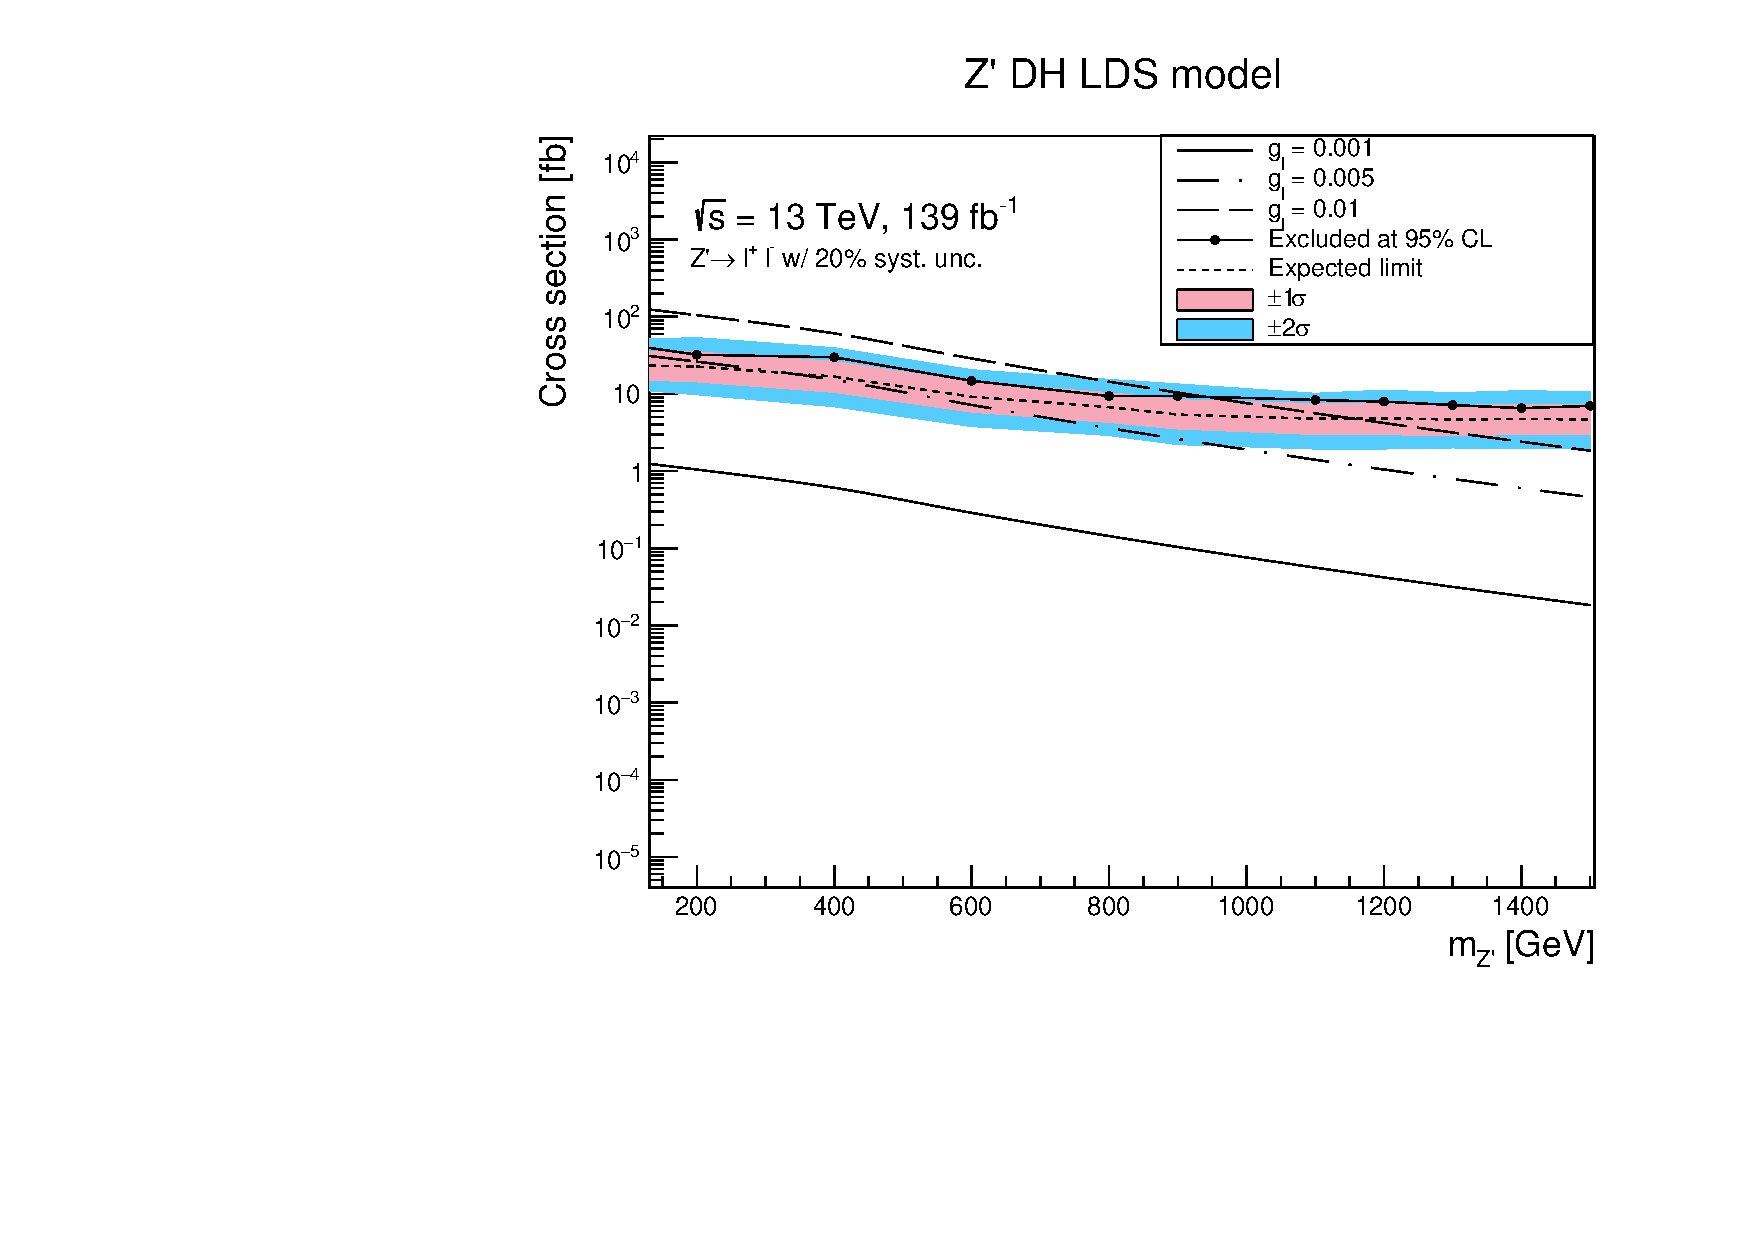
\includegraphics[width=1\textwidth]{Limits/DH_LDS/mass_exclusion_comb.pdf}
   \end{subfigure}
   \hfill
   \begin{subfigure}[b]{0.49\textwidth}
      \centering
      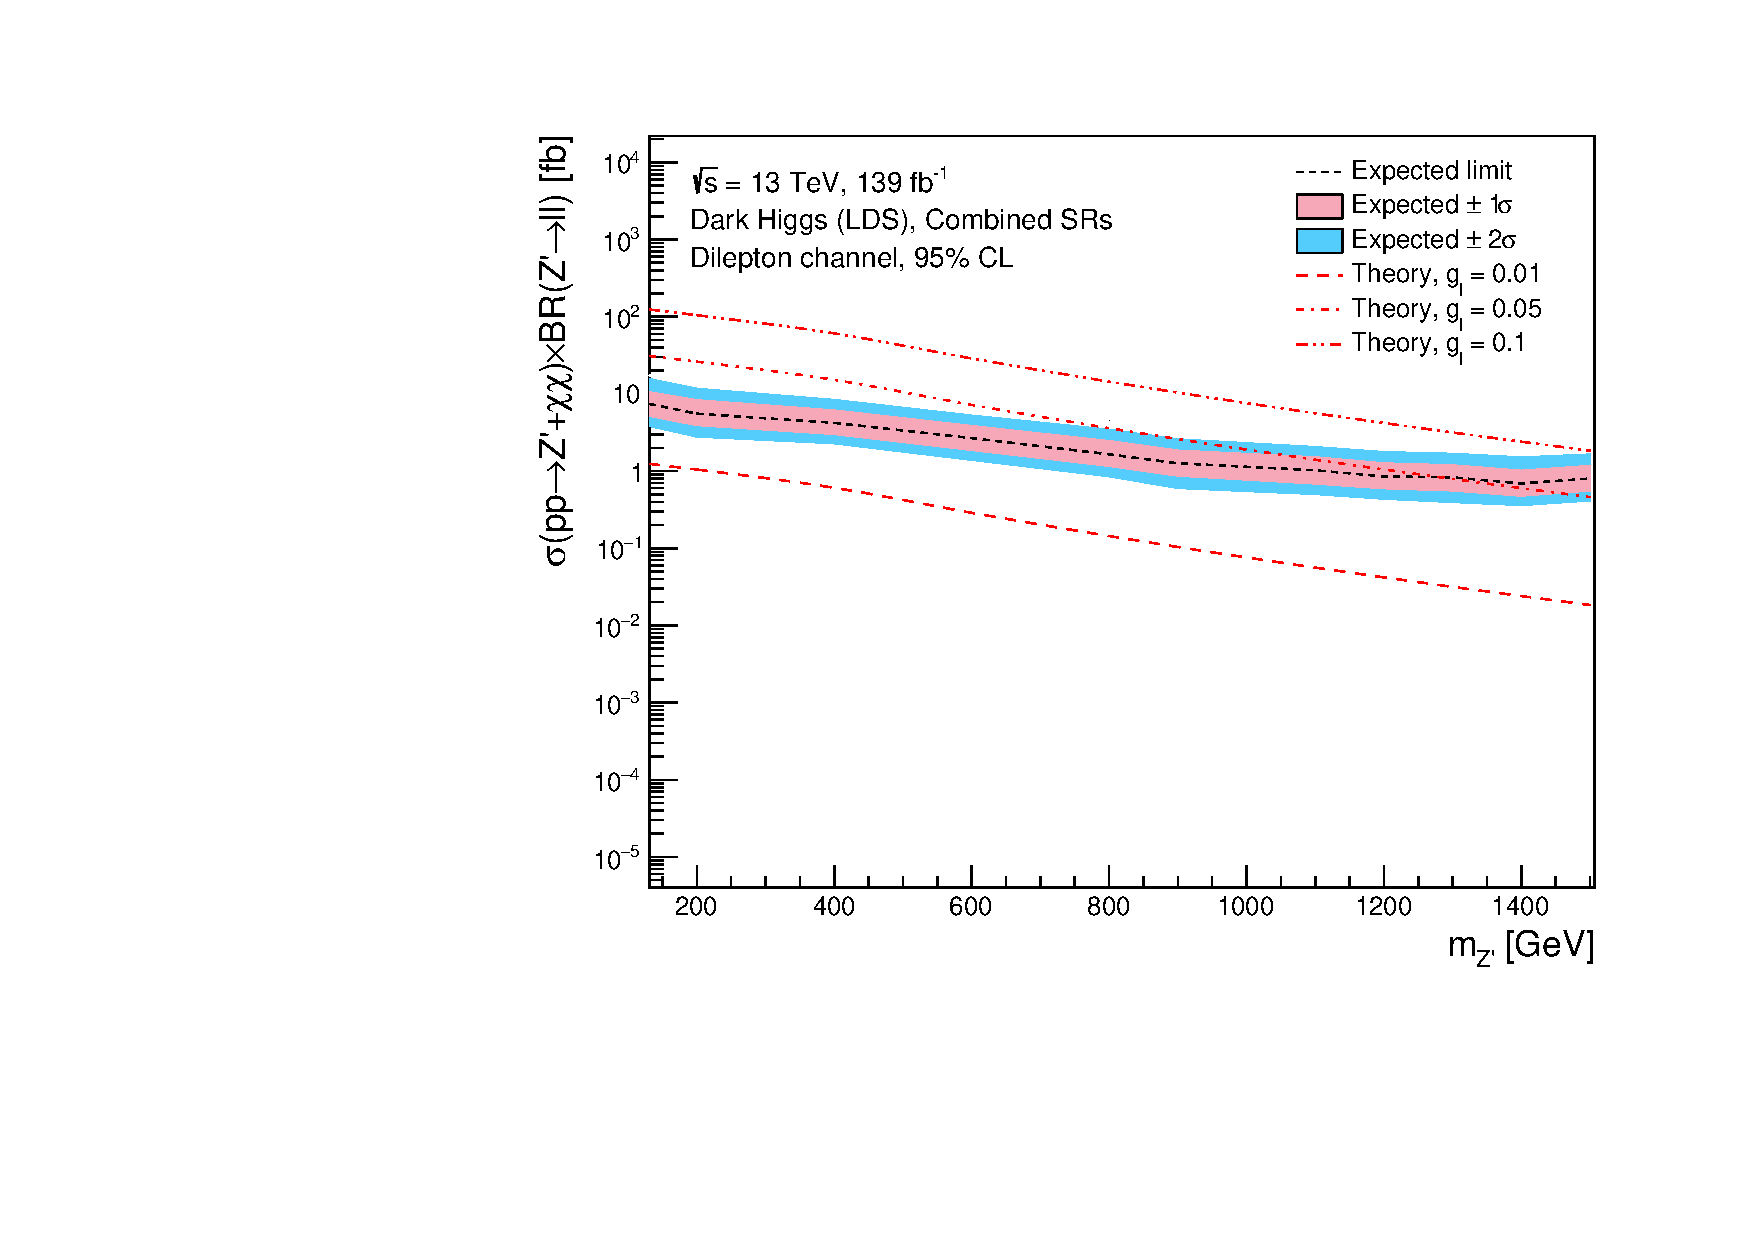
\includegraphics[width=1\textwidth]{Limits/Model_independent/DH_LDS/mass_exclusion_comb.pdf}
   \end{subfigure}
   \hfill
   \begin{subfigure}[b]{0.49\textwidth}
      \centering
      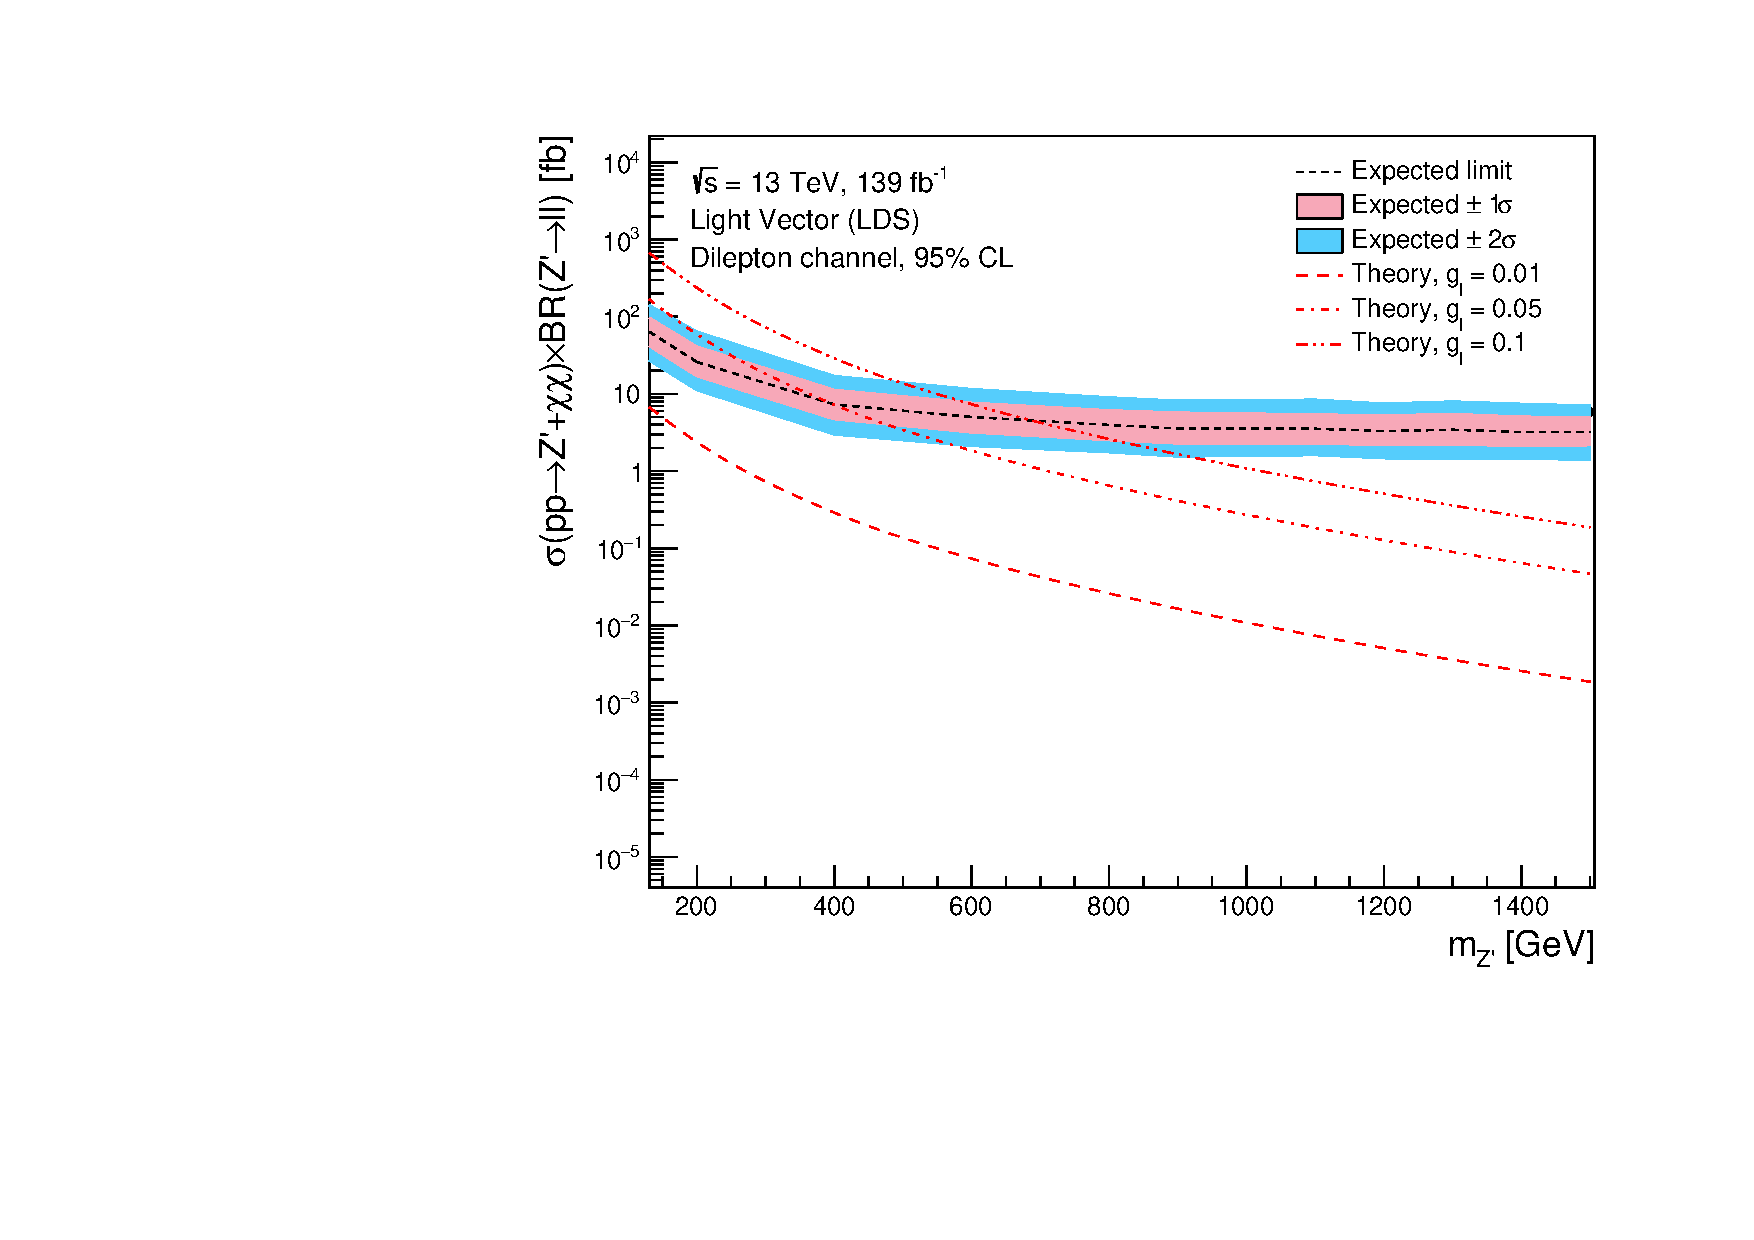
\includegraphics[width=1\textwidth]{Limits/LV_LDS/mass_exclusion_comb.pdf}
   \end{subfigure}
   \hfill
   \begin{subfigure}[b]{0.49\textwidth}
      \centering
      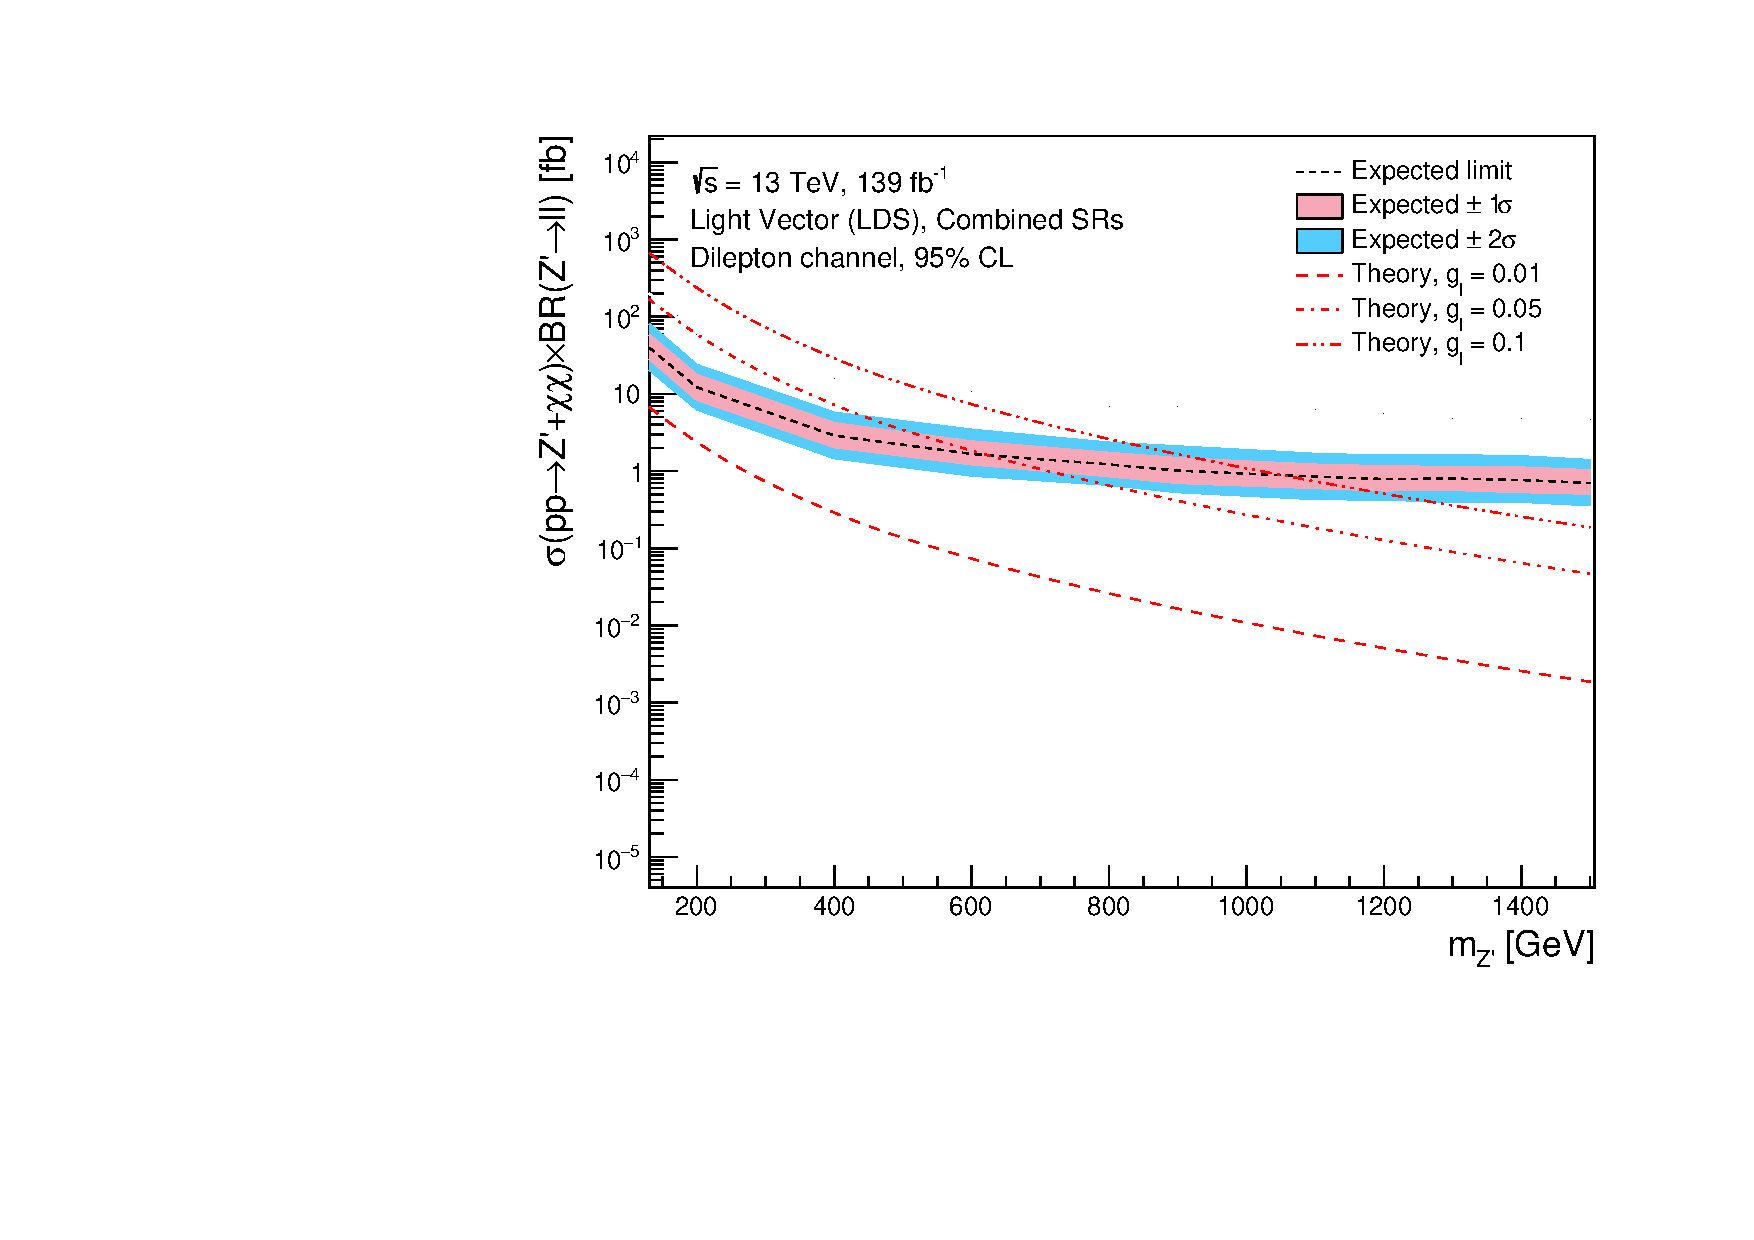
\includegraphics[width=1\textwidth]{Limits/Model_independent/LV_LDS/mass_exclusion_comb.pdf}
   \end{subfigure}
   \hfill
	\begin{subfigure}[b]{0.49\textwidth}
      \centering
      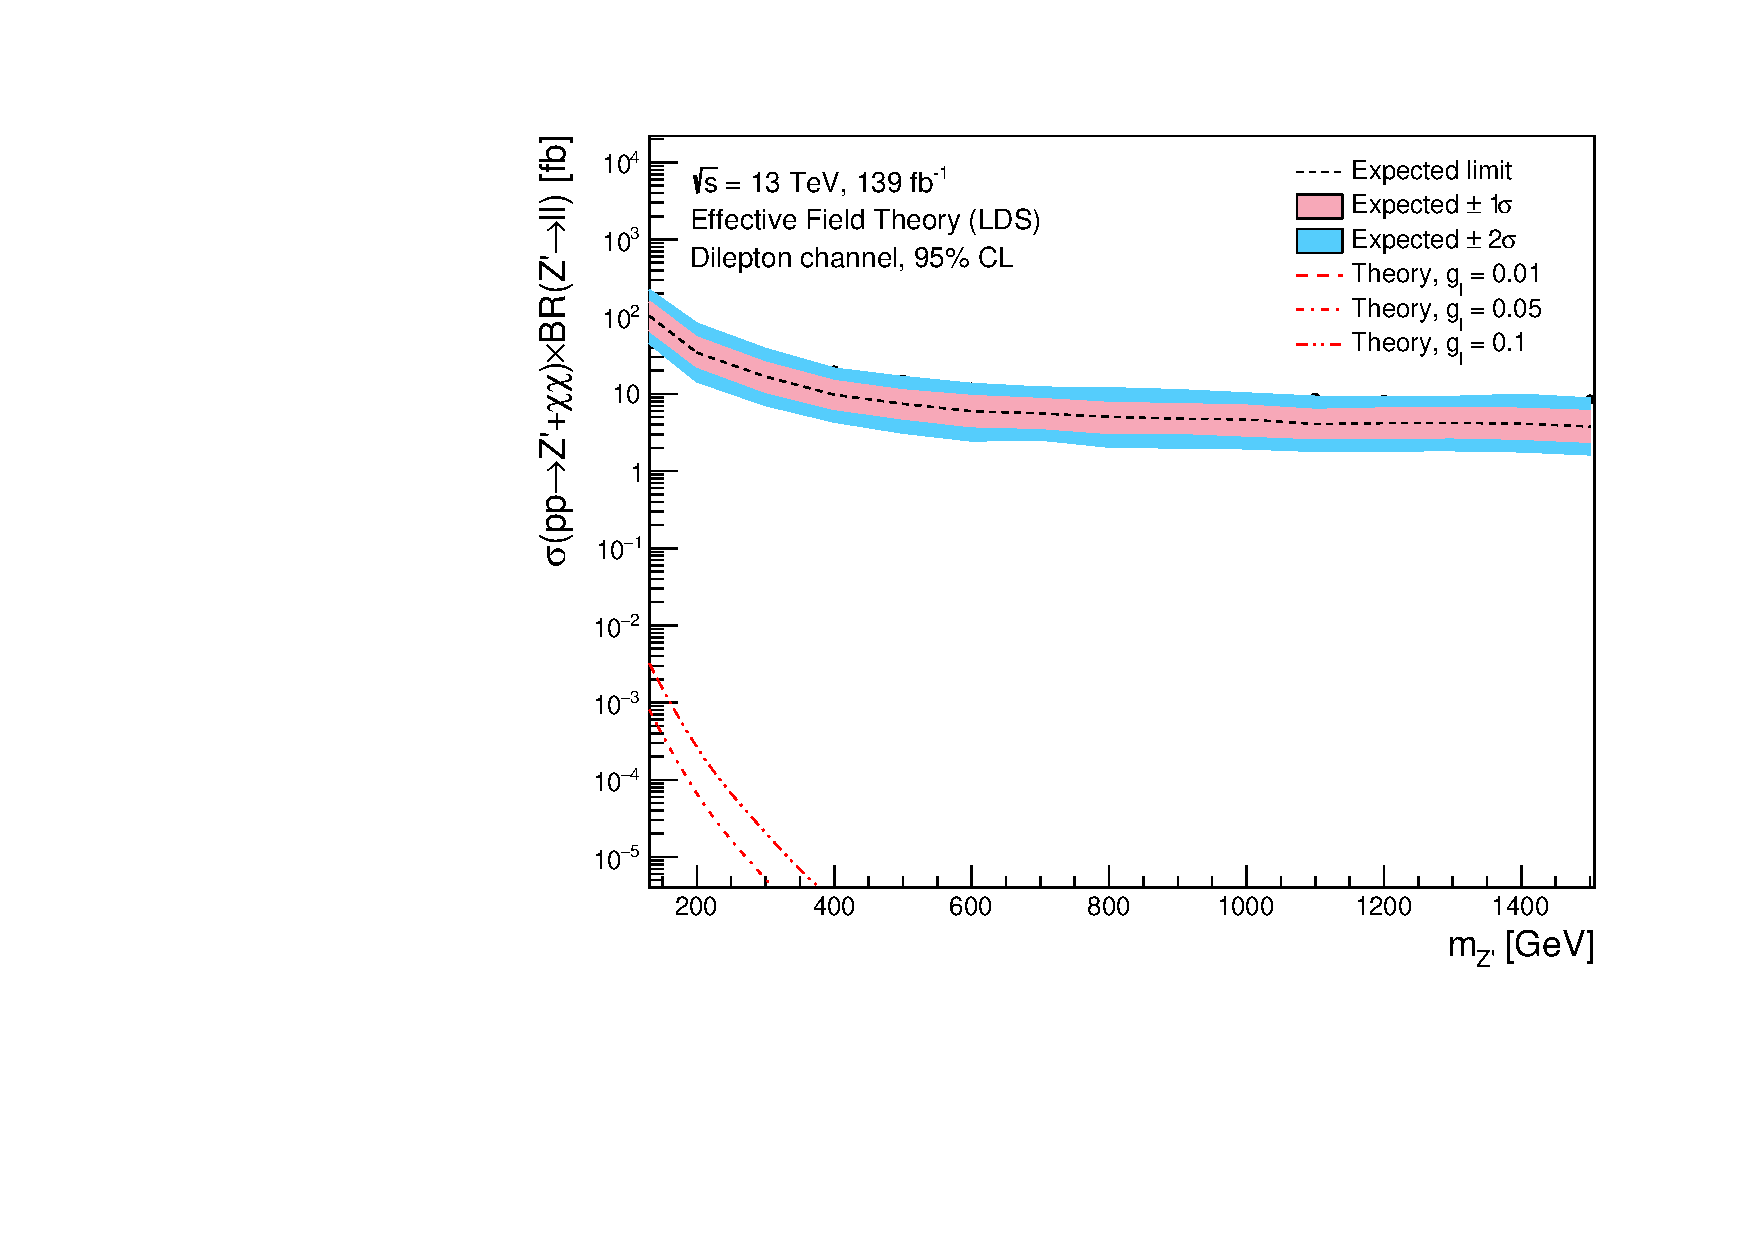
\includegraphics[width=1\textwidth]{Limits/EFT_LDS/mass_exclusion_comb.pdf}
   \end{subfigure}
   \hfill
   \begin{subfigure}[b]{0.49\textwidth}
      \centering
      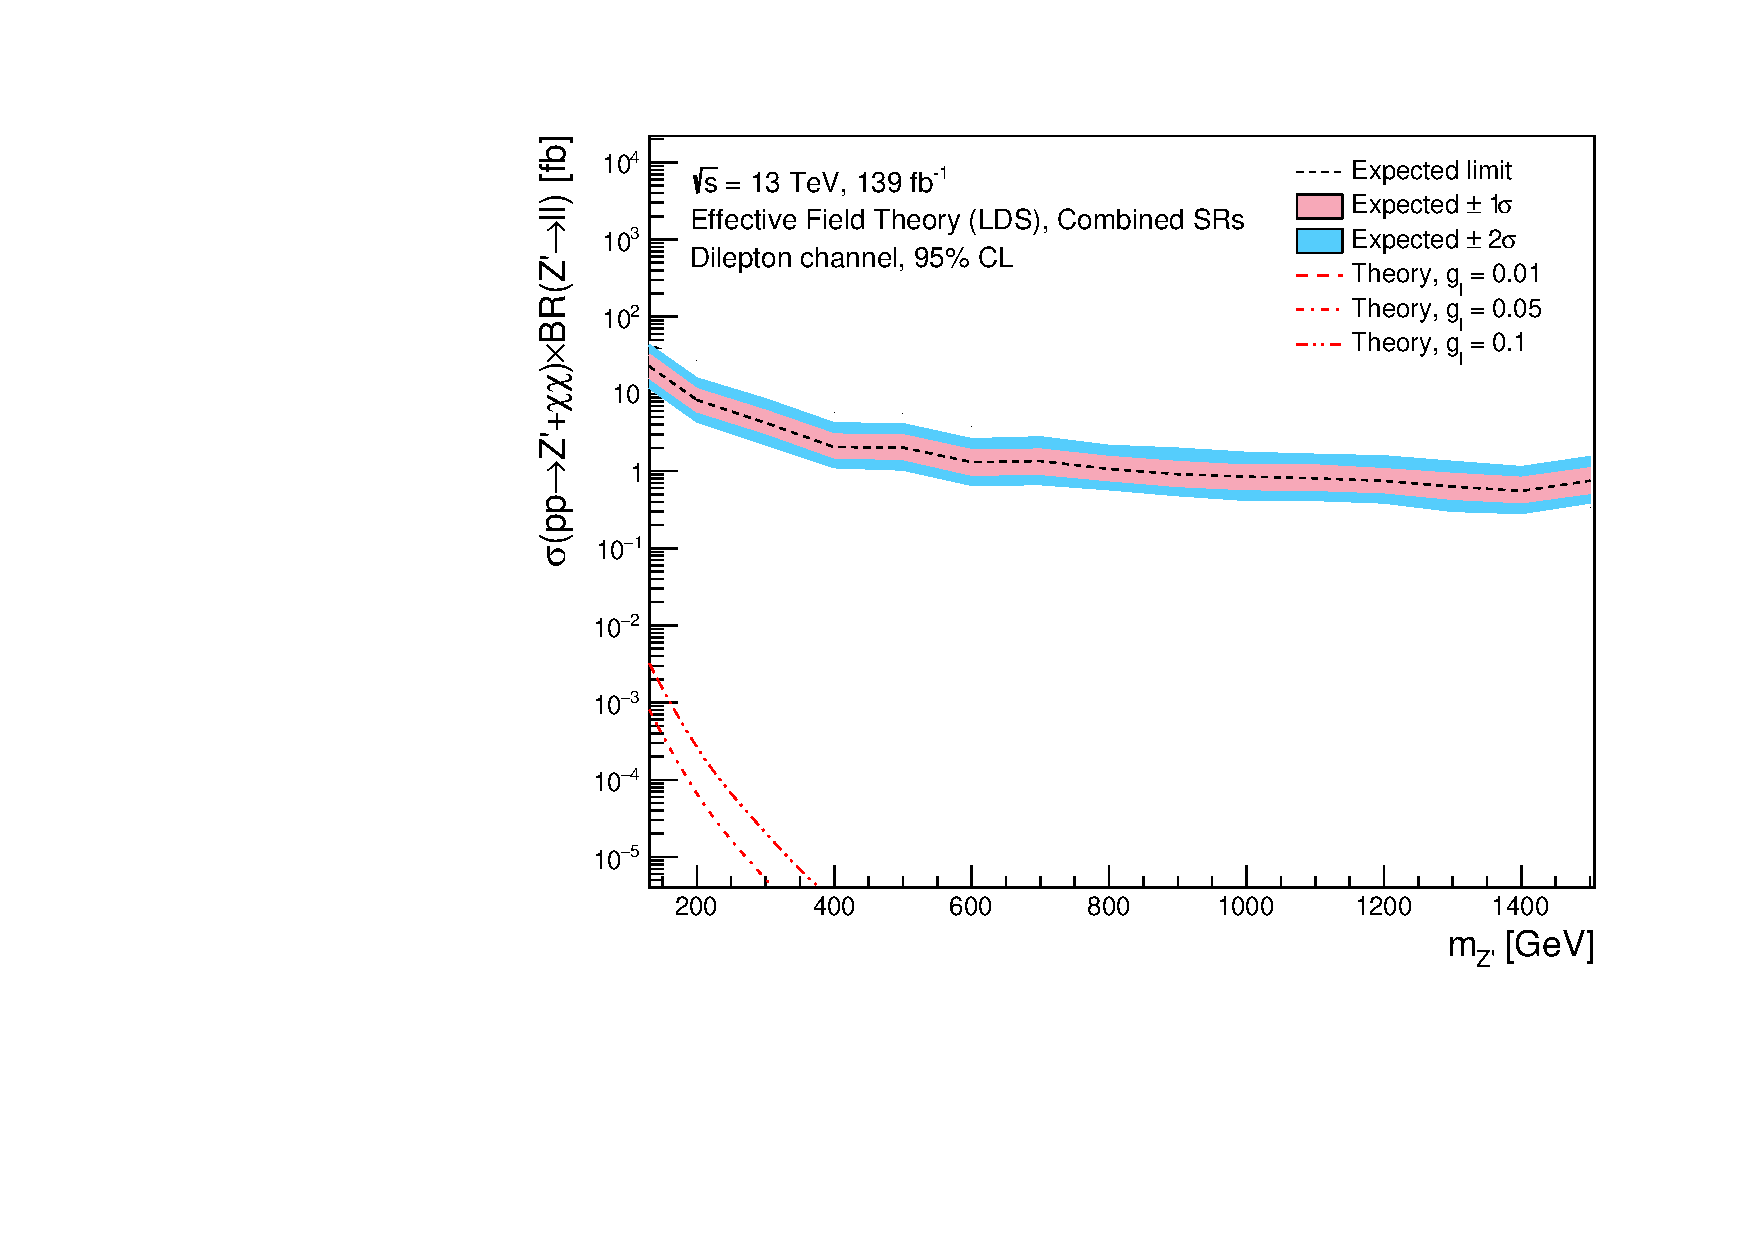
\includegraphics[width=1\textwidth]{Limits/Model_independent/EFT_LDS/mass_exclusion_comb.pdf}
   \end{subfigure}
   \caption[Comparison of mass exclusion limits of dilepton channel for all mono-Z' models using the model dependent and independent approach in the LDS]{Comparison of the mass exclusion limits of combined $ee$ and $\mu\mu$ channel for all mono-Z' models using the model dependent approach (left) and model independent approach (right) in the Light Dark Sector (LDS). 
   In the top row we have the mass exclusion of the Dark Higgs model. In the middle row we have the mass exclusions of the Light Vector model. In the bottom row we have the mass exclusion of the inelastic EFT model.
   The y-axis on all plots represents the cross-section times branching ratio of the process we are studying. The x-axis is the mass of the $Z'$ boson. We did not interpolate between the available masses we had simulated, 
   and have rather just connected the values calculated for each mass point by connecting the points. The dashed black line is the expected 95\% CL limit calculated using Bayesian statistics with a 1$\sigma$ and 2$\sigma$ deviation. 
   The different dashed lines represent the theoretical cross-section times branching ratio of the process when varying the value of the lepton coupling $g_l$ between the leptons and the $Z'$ boson. The simulated events in this thesis utilized the value $g_l=$ 0.01, we include the cross-section times branching ratio when increasing this coupling to 0.05 and 0.1 to see how the exclusions change. 
   }\label{fig:comp_LDS}
\end{figure}


\clearpage
\end{document}